\documentclass[12pt,PhD]{Thesis}
\usepackage{graphicx}
\usepackage{braket}
\usepackage{xspace}
\usepackage{ifpdf}
\usepackage{feynmp}
\usepackage{ifpdf}
\ifpdf
  \DeclareGraphicsRule{*}{mps}{*}{}
\fi
\usepackage{afterpage}
\usepackage{amssymb}
\usepackage{amsmath}
\usepackage{epstopdf}
\usepackage{epsfig}
\usepackage{grffile}
\usepackage{subfigure}
\usepackage{booktabs}
\usepackage[british]{babel}
\newcommand{\Pom}{I$\!$P}
\newcommand{\Reg}{I$\!$R}
\newcommand{\dr}{\mbox{$\Delta{\rm R}$}}
\newcommand{\deta}{\mbox{$\Delta{\rm \eta}$}}
\newcommand{\dphi}{\mbox{$\Delta{\rm \phi}$}}
\newcommand{\cosdphi}{\mbox{$\rm cos(\pi - \dphi{})$}}
\newcommand{\costwodphi}{\mbox{$\rm cos(2\dphi{}) $}}
\newcommand{\et}{\mbox{$E_{\rm t}$}}
\newcommand{\pt}{\mbox{$p_{\rm T}$}}
\newcommand{\ptave}{\mbox{$\pt{}^{ave}$}}
\newcommand{\kt}{\mbox{$k_{\rm t}$}}
\newcommand{\ptb}{\mbox{$\overline{p_{\rm T}}$}}
\newcommand{\dy}{\mbox{$\Delta y$}}
\newcommand{\qz}{\mbox{$Q_0$}}
\newcommand{\nb}{\mbox{$\bar{N}$}}
\newcommand{\gap}{\mbox{$f_{\rm gap}$}}
\newcommand{\Bold}[1]{\textbf{#1}}
\newcommand{\lumi}[1]{\mbox{$#1 \rm{cm}^{-2}\rm{s}^{-1}$}}
\newcommand{\etaphi}[1]{\mbox{$\Delta\eta \times \Delta\phi$ of $#1 \times #1$}}
\newcommand{\etaRange}[2]{\mbox{$#1<{\rm |\eta|}<#2$}}
\newcommand{\etarange}[2]{\mbox{$#1<{\rm \eta}<#2$}}
\newcommand{\Range}[3]{\mbox{$#2\le{\rm #1}\le#3$}}
\newcommand{\mean}[1]{\mbox{$\langle #1 \rangle$}}
\newcommand{\antikt}{\hbox{anti-${k_t}$}\xspace}
\newcommand{\Antikt}{\hbox{Anti-${k_t}$}\xspace}
\newcommand{\Incl}{\mbox{$\frac{1}{N}\frac{dN}{d\Delta y}$}}
\newcommand{\ptDist}{\mbox{$\frac{1}{N}\frac{dN}{d\Delta \pt{}^{veto}}$}}
\newcommand{\dphiDist}{\mbox{$\frac{d\sigma}{d\dphi{}}$}}
\newcommand{\dphidyDist}{\mbox{$\frac{d^2{}\sigma}{dyd\dphi{}}$}}
%\newcommand{\dphiDist}{\mbox{$d\sigma/d\dphi{}$}}


\submitdate{2012}

\dept{School of Physics and Astronomy}
\begin{document}
\title{Precision measurement of jets at ATLAS}
    \author{Gareth John Ashley Brown}
    \principaladviser{Prof. Fred Loebinger and Dr. Andrew Denis Pilkington}

\beforeabstract
\prefacesection{Abstract}
    This thesis describes the measurements of jet activity in the rapidity region between a dijet system formed in proton-proton collisions at a centre-of-mass energy of 7 TeV.
The data used were collected by the ATLAS detector during 2010 at the Large Hadron Collider at CERN.
A number of observables that probe additional quark and gluon radiation in the dijet topology were studied.

The development and performance of the monitoring system for the ATLAS calorimeter high level trigger is described.
The performance of the jet calibration and a study of the properties of jets in the forward calorimeter is also given.

The fraction of events that survive a veto on jets with transverse momentum above a jet veto scale, \qz{}, in the rapidity region between the dijet system is measured for dijets with mean transverse momentum $50<\ptb{}<500$ GeV and rapidity separation, \dy{}, of up to six.
The mean number of jets that have a transverse momentum above the jet veto scale in the rapidity region between the dijet system is also measured. 
These measurements are compared to state of the art theoretical calculations from HEJ and POWHEG, and also compared to PYTHIA, HERWIG++ and ALPGEN Monte Carlo generators.

The results of a preliminary analysis of dijet events with a large rapidity separation are given.
In this analysis azimuthal decorrelation variables have also been measured.

\afterabstract
  %  \prefacesection{The Author}
% Preface here
    %Author is Gareth

    %\prefacesection{Acknowledgements}
     %acknowledgements here
   % acknowledge

\afterpreface

\chapter{Introduction}
The study into dijet production with a jet veto is presented.
These observables are compared for a dijet rapidity separation of up to 6 units in rapidity, and $50\le\ptb{}<500$.
The data are compared to POWHEG with both the PYTHIA parton shower (POWHEG + PYTHIA) and the HERWIG parton shower (POWHEG + HERWIG), and also to the HEJ generator. 
The data are also compared to PYTHIA, HERWIG++ and ALPGEN.
A description of these genertors can be found in Section \ref{Theory:MC}.

The topology and event selection are outlined in Section \ref{sec:GBJ1:AnalSel} and \ref{sec:GBJ1:EvtSel}, respectively. 
In Section \ref{sec:GBJ1:DataStab}, the robustness of the event selection will be examined. 
In Section \ref{sec:GBJ1:Uncorr}, the selected data will be compared to the simulated PYTHIA sample.
Section \ref{sec:GBJ1:OtherWork} outlines the work done by other members of the analysis team that was required to get the final measurements, which are presented in Section \ref{sec:GBJ1:FinalPlots} and published in \cite{ref:ATLASGap}. 

%-introduction to the analysis
%   -define why we look at it
%   -what observables we want to look at
%
%-give a bit of info on what is going to be in each chapter


\chapter{Theory}
\label{chp:Theory}
The Standard Model (SM) of particle physics is the theoretical framework that describes the interaction of matter through the strong, electromagnetic, and weak forces.
Figure \ref{Theory:SM} shows the bosons and fermions in the SM.
The matter particles are represented in three generations of fermions, with particles in each generation being heavier than the previous. 
The electromagnetic force is mediated by the photon, which interacts with charged particles.
The weak force in mediated by the W and Z bosons.
The strong force describes the interactions between quarks and gluons, and is mediated by the gluon.
Finally, there is also the Higgs boson, which is the remnant of the Higgs field that was introduced to give mass to the bosons and fermions.
The strong force is described by QCD.
This thesis is concerned with QCD measurements, and more detail about QCD is given in this chapter.


\begin{figure}
\centering
\mbox{
              \epsfig{figure=figures/Theory/SM.eps,width=0.6\textwidth}
                              }
\caption[The fundamental particles in the Standard Model]{
The fundamental particles in the Standard Model.
\label{Theory:SM}}
\end{figure}


\section{QCD}
\label{Theory:QCD}
The QCD Lagrangian is given by 
\begin{equation}
\mathcal{L} = - \frac{1}{4} F^{a}_{\alpha\beta} F_{b}^{\alpha\beta} + \sum_{q} \bar{q}_{j}( i{\not}\partial - m_{q})q^{j}  + g_s\sum_{q} \bar{q}_{i}\gamma_{\mu} t^{a}_{ik} q^{k} A^{\mu}_{a}, 
\label{Theory:L_QCD}
\end{equation}
where $A^{\mu}_{a}$ is the gluon field, $t^{a}_{ik}=\frac{1}{2}\lambda_{a}$ with $\lambda_{a}$ being the Gell--Mann matrices, $\gamma_{\mu}$ are the gamma matrices, $m_{q}$ is the mass of the quark, $q$ and $\bar{q}$ are the spin half quark field and 
\begin{equation}
F^{a}_{\alpha\beta} = \partial^{\alpha}A_{A}^{\beta} - \partial^{\beta}A_{a}^{\alpha} + g_s f_{abc} A_{b}^{\alpha}A_{c}^{\beta}. 
\label{Theory:F_Tensor}
\end{equation}
Here, repeated indices imply summation. 
Greek characters represent Lorentz vector components and latin characters representing the different colour charge of the quarks and gluons. 

The first term in Equation \ref{Theory:L_QCD} is concerned with the gluon self coupling and gluon propagator. 
The product of $F^{a}_{\alpha\beta} F_{b}^{\alpha\beta}$ results in terms with $g^2$, which correspond to a four gluon interaction, terms with $g$, which correspond to the three gluon interaction and other terms that correspond to the basic gluon propagator.
The second term in Equation \ref{Theory:L_QCD} corresponds to the basic quark propagator without a gluon interaction.
The final term in Equation \ref{Theory:L_QCD} is the gluon-quark interaction.

\subsection{Asymptotic Freedom and Confinement}


The coupling constant, $\alpha_{s} = \frac{g_s^2}{4\pi}$, is used to quantify the strength of the partonic interactions.
%When strong interactions are calculated using perturbative QCD (pQCD), ultraviolet divergences arise which require a renormalisation. 
Renormalisation is required due to ultraviolet divergences that arise using perturbative QCD (pQCD). 
This procedure introduces an additional mass scale, $\mu$.
The coupling constant at a momentum scale, Q, relative to a scale $\mu$ at one-loop order is given by
\begin{equation}
\alpha_{s}(Q^2) = \frac{\alpha_{s}(\mu^2)}{1+b\alpha_{s}(\mu^2)\ln(\frac{Q^2}{\mu^2})}
\label{Theory:Coupling}
\end{equation}
where 
\begin{equation}
b = \frac{33-2n_f}{12\pi}
\label{Theory:b_Coupling}
\end{equation}
where $n_f$ is the number of active flavours of quarks and $b$ is positive for all flavours of quark in the SM.

The renormalisation scale $\mu$ is arbitrary and can be freely chosen.
Measurements of $\alpha_s$ are made at various values of $Q$ and are typically compared at $\alpha_s(M_{Z}^{2})\approx0.12$ \cite{ref:Webber}, where $M_Z$ is the mass of the Z.
This allows the calculation of $\alpha_s$ at other scales, though as Q gets small. 

The running of $\alpha_s$ with mass scale (Equation \ref{Theory:Coupling}) demonstrates two properties of QCD.
First, as the value of $Q$ increases, corresponding to probing smaller distances, the coupling constant becomes small and the quarks and gluons behaves as if they were free particles.
QCD therefore has asymptotic freedom.
Second, as $Q$ gets small, the coupling value of  $\alpha_s$ gets very large.
This hints towards the QCD feature known as confinement, which is the observation that quarks and gluons are always bound in colour neutral states, namely hadrons.

For theory calculations, pQCD should only be used down to a scale at which the perturbative expansion will likely no longer converge.
When modelling real-life events, it is used to define a perturbative region, where the calculation can be done using pQCD, and a non-perturbative region, where perturbation theory is no longer reliable and empirical models must be used. 


\subsection{Hadron -- Hadron Cross Section}

The QCD factorisation theorem suggests that the hadronic cross section of a given process can be split into the hard partonic scattering process, which can be calculated using pQCD, and a part that describes the non-perturbative structure of the hadron, characterised using the parton distribution functions (PDFs) \cite{ref:HardInt}.
The cross section for the process shown in Figure \ref{Theory:HadronHadron} is given by,
\begin{equation}
\sigma_{AB}=\int\int dx_a dx_b f_{a/A}(x_a) f_{b/B}(x_a) \hat{\sigma}_{ab\rightarrow X}
\label{Theory:XSec}
\end{equation}
where $A$ and $B$ are the initial protons, $a$ and $b$ are different combinations of quarks and gluons, $x_a$ is the fraction of the proton energy that parton $a$ carries, $ f_{a/A}(x_a)$ is the PDF which, to leading order, represents the probability of finding a parton with energy fraction  $x_a$ within A, and $\hat{\sigma}_{ab\rightarrow X}$ is the partonic cross section for the sub-process $ab\rightarrow X$.
The partonic cross section is given by
\begin{equation}
d \hat{\sigma}_{a,b\rightarrow X}= \frac{1}{\hat{s}}|\mathcal{M}_{a,b\rightarrow X}|^{2} d\Phi_n
\label{Theory:PartonCrossSection}
\end{equation}
where $a$ and $b$ represent the incoming partons, $\hat{s}= (k_a + k_b)^2$ where $k_i$ is the momentum of a parton $i$, $d\Phi_n$ is the n-body phase space, and $\mathcal{M}$ is the matrix element that is calculated using the Feynman rules \cite{ref:Webber}.
Where $X$ is a final state consisting of just quarks and gluons, then the Feynman rules can be derived only from the QCD Lagrangian. 

Problems occur when calculating collinear or soft gluon emission from the initial or final state, because infra-red (IR) divergences occur.  
A factorisation scale $\mu_F$ is defined such that emissions with a momentum less than $\mu_F$ are absorbed into the PDFs, and only emissions above this value are calculated. 
The PDFs have been measured at electron-proton collider and fix target experiments for a range of $x_0$ and $Q_0$ values \cite{ref:PDF1,ref:PDF2,ref:MRST}. 

\begin{figure}
\centering
\mbox{
              \epsfig{figure=figures/Theory/Hadron-Hadron.eps,width=0.6\textwidth}
                              }
\caption[Illustration of a hadron-hadron interaction]{
Illustration showing hadron-hadron interaction through partons $a$ and $b$ going to $X$. 
\label{Theory:HadronHadron}}
\end{figure}


\subsection{Jet Formation}

From the partonic cross section, the final state partons have energies $\mathcal{O}(\mu_{F})$.
From pQCD, it is expected that there is partonic emission off the final state partons, and the emission has a high probability if it is either soft or colinear. 
The resulting partons can also emit partons, and a partonic cascade occurs.
As discussed above, confinement requires that all observable particles are colour neutral, and this will only occur when there is a low relative momentum between partons.
This cascade continues until the partons are at the hadronic scale, $\mathcal{O}(1\rm GeV)$, and they bond into hadrons.
The result is a cascade of hadrons in the direction of the original parton.

Calculations with partons in the final state are performed using a jet algorithm.  
The jet algorithm clusters nearby partons into a single object.
The jet algorithms can be applied to calculations at a particular order in perturbation theory, to final state hadrons, or to detector deposits.
Figure \ref{Theory:InitJet} shows an illustration of a jet at different levels.


\begin{figure}
\centering
\mbox{
              \epsfig{figure=figures/Theory/JetEvolution.eps,width=0.9\textwidth}
                              }
\caption[Jets at parton, particle and calorimeter levels]{
Illustration of a jet at parton, particle and calorimeter levels. 
Illistration from Dag Gillberg.
\label{Theory:InitJet}}
\end{figure}


\section{Dijet Production}
\label{sec:Theory:Dijet}

The main analysis of this thesis is directed towards dijet production with a veto on additional jet radiation between the dijets.
Dijet production cross section can be calculated using Equation \ref{Theory:XSec} with the $\hat{\sigma}$ being the partonic cross section for $2\rightarrow 2$ scattering.
Measured dijet production cross sections as a function of the dijet kinematics, for instance the dijet mass, and can be compared to LO and NLO cross section calculations.
The dijet cross section is compared to NLO cross section calculation in \cite{ref:Dijet}, with an agreement within the experimental uncertainty.
The leading order (LO) cross section calculations have the lowest order of $\alpha_{s}$ needed to get the correct final state, for dijets this is $\alpha_{s}^{2}$.
Some of the LO parton scattering diagrams are shown in Figure \ref{Theory:LODijet}.
Next-to-leading order (NLO) cross section calculations consist of the LO cross sections with $\alpha_{s}^{2}$, plus the next order in the perturbative series expanded in $\alpha_{s}$, ie $\alpha_{s}^{3}$.
       \unitlength = 1mm
\begin{figure}
\centering
\mbox{
     
\begin{fmffile}{figures/QCD/gg1}
\begin{fmfgraph}(40,25)
\fmfleft{i1,i2}
\fmfright{o1,o2}
\fmf{gluon}{i1,v1,o1}
\fmf{gluon}{i2,v2,o2}
\fmf{gluon}{v1,v2}
\end{fmfgraph}
\end{fmffile}


\begin{fmffile}{figures/QCD/gg2}
\begin{fmfgraph}(40,25)
\fmfleft{i1,i2}
\fmfright{o1,o2}
\fmf{gluon}{i1,v1,o1}
\fmf{gluon}{i2,v1,o2}
\end{fmfgraph}
\end{fmffile}
     
     
    

\begin{fmffile}{figures/QCD/gg3}
\begin{fmfgraph}(40,25)
\fmfleft{i1,i2}
\fmfright{o1,o2}
\fmf{gluon}{i1,v1,i2}
\fmf{gluon}{o1,v2,o2}
\fmf{gluon}{v1,v2}
\end{fmfgraph}
\end{fmffile}

}

\enskip

\mbox{
 
   
%    Hello
%    
%\begin{fmffile}{gg4}
%\begin{fmfgraph}(40,25)
%\fmfleft{i1,i2}
%\fmfright{o1,o2}
%\fmf{phantom,tension=1.5}{i1,v1}
%\fmf{phantom,tension=1.5}{i2,v2}
%\fmf{phantom}{i1,v1,o1}
%\fmf{phantom}{i2,v2,o2}
%\fmf{gluon,tension=0}{i1,v1,o2}
%\fmf{gluon,tension=0,rubout}{i2,v2,o1}
%\fmf{gluon}{v1,v2}
%\end{fmfgraph}
%\end{fmffile}


    

\begin{fmffile}{figures/QCD/qq1}
\begin{fmfgraph}(40,25)
\fmfleft{i1,i2}
\fmfright{o1,o2}
\fmf{fermion}{i1,v1,i2}
\fmf{fermion}{o1,v2,o2}
\fmf{gluon}{v1,v2}
\end{fmfgraph}
\end{fmffile}
     
     
       

\begin{fmffile}{figures/QCD/qq2}
\begin{fmfgraph}(40,25)
\fmfleft{i1,i2}
\fmfright{o1,o2}
\fmf{fermion}{i1,v1,i2}
\fmf{gluon}{o1,v2,o2}
\fmf{gluon}{v1,v2}
\end{fmfgraph}
\end{fmffile}
     
     

\begin{fmffile}{figures/QCD/qq3}
\begin{fmfgraph}(40,25)
\fmfleft{i1,i2}
\fmfright{o1,o2}
\fmf{fermion}{i1,v1}
\fmf{fermion}{v2,i2}
\fmf{fermion,tension=0}{v1,v2}
\fmf{gluon}{v2,o2}
\fmf{gluon}{v1,o1}
\end{fmfgraph}
\end{fmffile}

}

\enskip


\mbox{



\begin{fmffile}{figures/QCD/qq4}
\begin{fmfgraph}(40,25)
\fmfleft{i1,i2}
\fmfright{o1,o2}
\fmf{fermion}{i1,v1,o1}
\fmf{fermion}{i2,v2,o2}
\fmf{gluon,tension=0}{v1,v2}
\end{fmfgraph}
\end{fmffile}
                              }
\caption[LO Feynman diagrams for dijet production]{
Some of the LO Feynman diagrams for dijet production. 
The straight lines represent quarks, and the curly lines represent gluons.
The arrows on the fermion lines going from left-to-right and right-to-left distinguish quarks and anti-quarks respectively.
\label{Theory:LODijet}}
\end{figure}






When describing pp collisions, it is useful to define a co-ordinate system.
The z-direction is defined as the collision axis, with the x-y plane defined perpendicular to the collision azis.
For an object with energy, E, and momentum, $\bold{\rm p}$, the rapidity, $y$, of the object is defined by
\begin{equation}
y=\frac{1}{2}\ln\left(\rm \frac{E+p_z}{E-p_z}\right)
\label{Theory:Rapidity}
\end{equation}
where $\rm p_{z}$ is the longitudinal z component of momentum. 
The azimuthal angle, $\phi$, is defined as the angle in the x-y plane around the collision axis.
The transverse momentum, \pt{}, is defined as
\begin{equation}
\pt{}=\sqrt{ p_{x}^{2} +  p_{y}^{2}}.
\label{Theory:pt}
\end{equation}
Both \pt{} and differences in rapidity are Lorentz invarient in boosts in the z-direction \cite{ref:Rapidity}.  
 

To study the additional radiation in the dijet region, the fraction of events that do not contain an additional jet between the dijet is measured.
This is the gap fraction, defined as
\begin{equation}
f_{gap}(Q_{0}) = \frac{\sigma_{0}}{\sigma},
\label{Theory:GapFraction}
\end{equation}
where $\sigma$ is the dijet cross section,  $\sigma_{0}$ is the cross section for a dijet system without a parton with \pt{} above the jet veto scale, $\qz{}$, in the rapidity region spanned by the dijet system.
The gap fraction is studied as a function of the dijet rapidity separation, \dy{}, the average transverse momentum of the dijet, \ptb{} and the veto scale, \qz{}.
The dependence of the gap fraction on \dy{}, \ptb{}, and \qz{} is studied after keeping two of the variables fixed.

The dijet cross section can be calculated at fixed order using pQCD.
However, for some regions of the dijet kinematics or veto jet scale, the pQCD calculation of $\sigma_{0}$ requires increasing number of higher order terms, and so a resummation is done.
Figure \ref{Theory:KineRange} illustrates the different effects that need to be considered for different regions of the dijet kinematics and jet veto scale.
In particular, putting the dijet kinematics to high \dy{} or to large values of $Q/\qz{}$ require sophisticated calculation tools, and resummation to all orders in perturbation theory is necessary \cite{ref:Jeff3,ref:HEJ1}.

A number of other variables are used to probe the effect of higher order QCD.
The azimuthal decorrelation variables probe how back-to-back a pair of jets are.
For leading order dijet production, they are back-to-back, but emission change this and move them away from back-to-back.
The azimuthal decorrelation observables considered in this thesis are \dphiDist{}, \mean{\cosdphi{}} and  \mean{\costwodphi{}} hich were proposed by theorists  \cite{ref:BFKL,ref:BFKL_cos,ref:BFKL_dPhi,ref:Anderson1}.  
The mean number of jets in the rapidity region spanned by the dijet system is another probe of higher order QCD, and suggested by theorists \cite{ref:Andersen2}.



\begin{figure}
\centering
\mbox{
              \epsfig{figure=figures/Theory/LY.pdf,width=0.9\textwidth}
}
\caption[]{
Illustration depicting what type of physics is important for the gap fraction calculation for dijet rapidity separation, Y, and $L=\ln(Q/\qz{})$.
Figure taken from \cite{ref:Forshaw_Veto}.
\label{Theory:KineRange}}
\end{figure}
%To study the emmision of radiation a veto on additional jets between the dijet can be applied.


%If an event has no jet between the dijets, it is descrived as a gap event, and 




\section{Jets}
\label{sec:Theory:Jets}

Jets are defined using a jet finding algorithm which attempts to cluster nearby objects together.
For a jet finding algorithm to be theoretically safe it need create the same jet independent of what level it is running over, for instance partons, hadrons, and energy deposits.
The algorithm also needs to be both collinear and infrared safe.
Collinear safety of a jet is the requirement that the jet finding should be unaffected by particles radiated at small angles to the original particle. 
Figure \ref{Theory:IR} is a illustration of a collinear unsafe jet finding algorithm with a minimum \pt{} requirement of the objects.
In the case where there is only one object, the \pt{} is  greater than the \pt{} cut and only one jet is found. 
If the object splits into two collinear objects no jet is found, as the splitted objects do not pass the \pt{} cut.
Infrared safety requires that the jet finding is unaffected by the addition of soft radiation in the event.  
Figure \ref{Theory:Collinear} is an illustration of (a) two jets formed around two objects. 
The effect on the final jet state due to additional soft objects between the objects is shown for (b) an IR safe and (c) IR unsafe jet finding algorithm.


\begin{figure}
\centering
\mbox{
              \subfigure[]{\epsfig{figure=figures/Theory/Original-Collinear.eps,width=0.3\textwidth}}\quad
              \subfigure[]{\epsfig{figure=figures/Theory/Unsafe-Collinear.eps,width=0.3\textwidth}}\quad
                              }
\caption[]{
Illustration of a jet finding algorithm which requires the objects has a minimum \pt{} before jet finding. 
(a) is a jet found around a object and (b) shows the effect of splitting the object into two smaller objects.
The lengths of the arrowed lines represents the relative \pt{} of the objects and the green line is the minimum object \pt{}.
\label{Theory:IR}}
\end{figure}

\begin{figure}
\centering
\mbox{
              \subfigure[]{\epsfig{figure=figures/Theory/Original-IR.eps,height=0.3\textwidth}}\quad
              \subfigure[]{\epsfig{figure=figures/Theory/Safe-IR.eps,height=0.3\textwidth}}\quad
              \subfigure[]{\epsfig{figure=figures/Theory/Unsafe-IR.eps,height=0.3\textwidth}}\quad
                              }
\caption[]{
Illustration showing (a) jet finding on two objects and the effect on the jet final state of additional soft object between the two objects for (b) an infrared safe and (c) an infrared unsafe jet finding algorithm. 
\label{Theory:Collinear}}
\end{figure}


\subsection{\Antikt{} jets}

The main jet finding algorithm used in ATLAS is the \antikt{} algorithm \cite{ref:antiKt}, which is a sequential recombination algorithm.
The algorithm defines 
\begin{equation}
d_{ij} = min\left( \frac{1}{\kt{}_j^2},\frac{1}{\kt{}_i^2}\right) \frac{\Delta R_{ij}^2}{R^2}
\label{Theory:dij}
\end{equation}
and 
\begin{equation}
d_{iB} = \frac{1}{\kt{}_i^2}
\label{Theory:diB}
\end{equation}
for all objects (for example partons, particles, energy deposits) in the event.

The algorithm then combines the objects into jets in the following way:

\begin{enumerate}
\item Find the smallest of $d_{ij}$ and $d_{iB}$
\item If $d_{ij} < d_{iB}$ then combine the two objects
\item If $d_{ij} > d_{iB}$ then define object $i$ as a jet and remove from list of objects
\item Continue iterating until there is no objects left 
\end{enumerate}

The jet finding algorithm combines the highest \pt{} objects first, which have a  $\Delta R  < R$, then subsequently lower \pt{} objects.
Only jets that have a final \pt{} greater than a \pt{} cut are kept in the jet collection. 

There are many algorithms that are theoretically safe (both IR and collinear safe).
The \antikt{} algorithm was chosen to be the default because it produces regularly shaped jets and has a good behaviour under noise and pileup. 
In ATLAS the default is to uses two $R$ parameters, 0.4 and 0.6, and full four momentum recombination.

%\subsection{Parton Hadron Duality}

\section{MC Event Simulation}
\label{Theory:MC}


Monte Carlo (MC) event simulation is used to compare data to theoretical predictions. 
MCs aim to give a full description of a hadron-hadron interaction.
As discussed in Section \ref{Theory:QCD}, the calculation can be factorised to separate the perturbative and non-perturbative parts. 
First the differential partonic cross section is calculated to model the kinematics of the hard interaction.
This will typically consist of $n$ high \pt{} partons in the final state.
Parton showering and hadronisation algorithms are used to turn the partonic final state into a hadronic one.

PS attempts to simulate the higher order contributions to the calculation from soft and collinear parton emission.
There is a greater probablity of emisson for soft or collinear emission from the partons.
The effectiveness of the PS for soft and collinear emissions is tested through jet shapes \cite{ref:JetSh}.
The PS correctly resums soft and collinear contributions, is to leading logs.
Through the parton showering, the high \pt{} partons successively radiates partons until all partons are at a scale of a few GeV.
Once at this scale, hadronisation combines the partons together to make colour neutral hadrons. 

MC often include emission from multiple parton-parton interactions (MPI), which is included in the event before the hadronisation.



\subsection{MC Generators}
\subsubsection{PYTHIA}

PYTHIA \cite{ref:PYTHIA64} is a general-purpose MC with a large library of LO sub-processes, including the LO QCD matrix elements for the $2 \rightarrow 2$ sub-processes used for dijet production.
The PYTHIA PS orders emissions in transverse momentum and has a veto to ensure angle ordering. 
The hadronization used in PYTHIA is based on the Lund string model \cite{ref:Lund}.
The version of PYTHIA used in the analyses presented is PYTHIA 6.4.2.3 with the MRST LO$^*$ PDF \cite{ref:MRST} and the AMBT1 tune \cite{ref:Tune}.

The dijet cross section is falling in both \ptb{} and \dy{}.
To get a large number of events in the high \ptb{} and \dy{} regions, a filter is applied to the centrally produced PYTHIA samples used in Chapters \ref{chp:GBJ1,chp:GBJ2}. 
The result of the filter is flat distribution in \ptb{} and \dy{}. 
Event weighting factors are stored which allows the original distribution to be recovered. 

To improve the decription of data, multiple proton-proton intereaction, ``pile-up'', is included.

Unlike the other MC generators considered, the PYTHIA events are passed through a full ATLAS detector simulation, based on GEANT4 \cite{ref:Geant4}, which results in a sample of fully simulated events which can be directly compared to data. 

\subsubsection{HERWIG++}

HERWIG++ is another general-purpose MC which has LO QCD matrix elements for the $2 \rightarrow 2$ sub-processes.
HERWIG++ has a PS which evolves the partons using angular ordering of emissions.
The hadronization used in HERWIG is the cluster model \cite{ref:ClusterModel} which forces all the gluons remaining from the PS to split into quark anti-quark pairs. 
The version used is HERWIG++ 2.5.0 \cite{ref:HERWIG} using the MRST LO$^*$ PDF and underlying event tune of LHC-UE7-1 \cite{ref:Herwigpp}. 
\subsubsection{ALPGEN}

The ALPGEN \cite{ref:ALPGEN} MC generator provides leading order matrix elements for up to 6 partons in the final state.
The ALPGEN sample was generated with the CTEQ6L1 PDF set \cite{ref:ALPGENPDF}.
The sample was pass through HERWIG and JIMMY \cite{ref:Jimmy} for parton showering, hadronization and MPI with AUET1 tune \cite{ref:ALPGENTune}.

\subsubsection{POWHEG}
The POWHEG generator \cite{ref:Powheg1,ref:Powheg2,ref:Powheg3} has the NLO matrix elements for dijet production. 
This MC is then interfaced to both PYTHIA and HERWIG for parton showering, hadronization and MPI.
Events were generated with the MSTW 2008 NLO PDF.


\subsubsection{HEJ}
High Energy Jets (HEJ) \cite{ref:HEJ1,ref:HEJ2} is a parton level generator. 
HEJ implements an all-order description of hard wide-angle emissions, in which parton emisions are ordered in rapidity.
Due to this, HEJ is expected to model the data well in th large \dy{} region in Figure \ref{Theory:KineRange}.
Events were generated with the MSTW 2008 NLO PDF.





\chapter{The LHC and ATLAS}
\label{chp:LHC_ATLAS}
The basic properties of the LHC are summarised in section \ref{sec:Det:LHC}. 
Sections \ref{sec:Det:Coord} and \ref{sec:Det:Over} define the ATLAS coordinate system and give a brief overview of the detector, working outwards from the beam line.
Those components of the detector of particular relevance to this analysis are described in more detail in Section \ref{sec:Det:Cal} and \ref{sec:Det:Trig}.

\section{The Large Hadron Collider}
\label{sec:Det:LHC}

The Large Hadron Collider (LHC) is situated 100 m below the border between Switzerland and France near the Swiss city of Geneva. 
The LHC was designed to provide two proton beams with 2808 bunches in each beam colliding with 25 ns bunch spacing at a centre-of-mass energy of 14 TeV.
Around the LHC ring, which is 26.6 km long, there are four interaction points. 
The four experiments at these interaction points are ATLAS, CMS, LHCb and ALICE.
ATLAS and CMS are general purpose detectors designed to be able to detect a broad range of physics processes. 
ALICE is designed to investigate heavy ion collisions, and LHCb is designed to explore CP violation and rare B-decays.
Figure \ref{Det:LHC} shows the layout of the LHC, and the four experiments.

\begin{figure}
\centering
\includegraphics[width=0.9\textwidth]{figures/Detector/AtlasSite.jpg}
  \caption[The Large Hadron Collider complex]{
The Large Hadron Collider and the sites of the 4 main LHC experiments.
\label{Det:LHC}
}
\end{figure}

A series of accelerators provide proton bunches to the LHC at an energy of 450 GeV.
The proton bunches are then accelerated around the LHC by an array of superconducting dipole magnets to provide a beam energy up to 7 TeV.
The beam energy during the 2010 and 2011 proton-proton collisions was 3.5 TeV, in 2012 it was 4 TeV.


\subsection{Luminosity}

The event rate for $pp \rightarrow X$ is
\begin{equation}
R_X = L \sigma_X,
\label{Det:Lumi}
\end{equation}
where $\sigma_X$ is the cross-section for the process and $L$ is the instantaneous luminosity.
Achieving a large integrated luminosity,
\begin{equation}
{\cal L} = \int L\cdot dt,
\label{Det:IntLumi}
\end{equation}
is important for observing rare physics processes that have a low cross-section. 
Accurate luminosity determination is important for measuring differential cross-sections of processes from the event rate. 

Instantaneous luminosity is defined by,
\begin{equation}
L=\frac{N_b^2n_bf_{rev}\gamma_r}{4\pi\epsilon_n\beta^\star}F,
\label{Det:Lumi}
\end{equation}
where $N_b$ is the number of particles per bunch, $n_b$ is the number of colliding bunches per beam, $f_{rev}$ is the revolution frequency, $\gamma_r$ is the relativistic gamma factor, $\epsilon_n$ is the normalised transverse beam emittance, $\beta^\star$ is the $\beta$ function at the interaction point, and $F$ is the geometric luminosity reduction factor due to the crossing angle of the beams.


Equation \ref{Det:Lumi} is useful to understand both the luminosity and how to increase it. 
Experimentally, the instantaneous luminosity can be determined by measuring the interaction rate in various ATLAS sub-detectors.
The luminosity defined by the interaction rate is,
\begin{equation}
L=\frac{\mu n_bf_{rev}}{\sigma_{inel}}=\frac{\mu_{vis}n_bf_{rev}}{\sigma_{vis}}
\label{Det:Lumi2}
\end{equation}
where $\mu$ is the number of inelastic collisions per bunch crossing, $\sigma_{inel}$ is the inelastic cross-section, $\mu_{vis}$ is the number of visible inelastic collisions per bunch crossing, and $\sigma_{vis}$ is a calibration constant related to the visible inelastic cross-section. 
This is obtained in special runs using Van der Meer scans and provide a luminosity uncertainty of 3.4\% \cite{ref:Lumi}.

\subsubsection{2010 run}
The 7 TeV centre-of-mass proton-proton run in 2010 was the first substantial data-taking period provided by the LHC. 
The initial runs provided peak luminosity of \lumi{\approx0.01\times10^{30}} from one pair of interacting bunches with a very low number of protons per bunch. 
By the end of the 2010 data-taking run, the peak luminosity was \lumi{\approx2\times10^{32}} from 348 colliding bunches.
The luminosity increase was mainly achieved by increasing the number of colliding bunches per beam and the number of protons per bunch, though decreasing the $\beta^\star$ and reducing the beams crossing angle also increased the luminosity.

The data is split into luminosity blocks, runs and periods.
A luminosity block corresponds to the luminosity information stored in two minute intervals during a run. 
A data run is a group of luminosity blocks consecutively taken. 
A data period is a group of data runs with similar beam parameter conditions.

The 2010 data taking run was split into nine different data periods, which corresponded to a total integrated luminosity delivered of 48.1 $\rm pb^{-1}$.
Table \ref{Det:Periods} shows the data periods for the 2010 LHC run, and how the beam conditions and peak luminosity changed.  
In addition, periods G-I used bunch trains where bunches are grouped together with 150 ns spacing between the bunches.  
As instantaneous luminosity increased, the level of ``pile-up'', which is multiple proton-proton interactions in the same bunch crossing, increased.

\begin{table}
\begin{center}
\begin{tabular}{|c|c|c|c|c|}
\hline
Period&Date&Peak Luminosity& $N_b$ & $n_b$ \\
& &\lumi{}& $\times10^{11}$ & \\
\hline
A & Mar 30 - Apr 18 & 0.004 & $<0.01$ & 1 \\
B & Apr 23 - May 17 & 0.06 & 0.01-0.6 & 1-3 \\
C & May 18 - June 5 & 0.2 & 0.7-1.9 & 3-8 \\
D & June 18 - July 19 & 1.6 & 3-8 & 2-8 \\
E & July 29 - Aug 18 & 3.9 & 12-14 & 16 \\
F & Aug 19 - Aug 30 & 10 & 35-100 & 32-36 \\
G & Sept 22 - Oct 7 & 70 & 100-200 & 50-186 \\
H & Oct 8 - Oct 18 & 150 & 250-350 & 233-300 \\
I & Oct 24 - Oct 29 & 210 & 350-400 & 300-350 \\
\hline
\end{tabular}
\caption[2010 Data Period Information]{
   Beam information for the different data taking periods in 2010 data.
\label{Det:Periods}
}
\end{center}
\end{table}


\section{The ATLAS Coordinate System}
\label{sec:Det:Coord}
The ATLAS experiment uses a right-handed Cartesian coordinate system. 
The beam line defines the $z$-axis, with the $x$-$y$ plane being perpendicular to this. 
The positive $x$ direction is defined going from the interaction point to the centre of the LHC ring. 
The positive $y$ direction points upwards from the interaction point. 
The detector side in the positive $z$ direction is called A and the side in the negative $z$ direction C.
The azimuthal angle, $\phi$, is defined as the angle in the $x$-$y$ plane around the beam, and the polar angle, $\theta$, is the angle to the beam line.
Using the polar angle, pseudorapidity $\eta$ is defined by 
\begin{equation}
\eta = - \ln \tan \left(\frac{\theta}{2}\right).
\label{Detector:eta}
\end{equation}
Pseudorapidity provides a close approximation to the rapidity defined in Equation \ref{Theory:Rapidity}.
The angle between two objects, $\Delta R$, is defined by 
\begin{equation}
\Delta R = \sqrt{(\Delta \eta)^2+(\Delta \phi)^2} .
\label{Detector:dR}
\end{equation}

All transverse variables (such as transverse momentum, $p_T$, and transverse energy, $E_T$) use only the $x$ and $y$ components of the variable and so are defined in the $x$-$y$ plane.

\section{The ATLAS Detector}
%The designed peak luminosity for the LHC to provide at the ATLAS interaction point is \lumi{1\times10^{24}}.

\begin{figure}
\centering
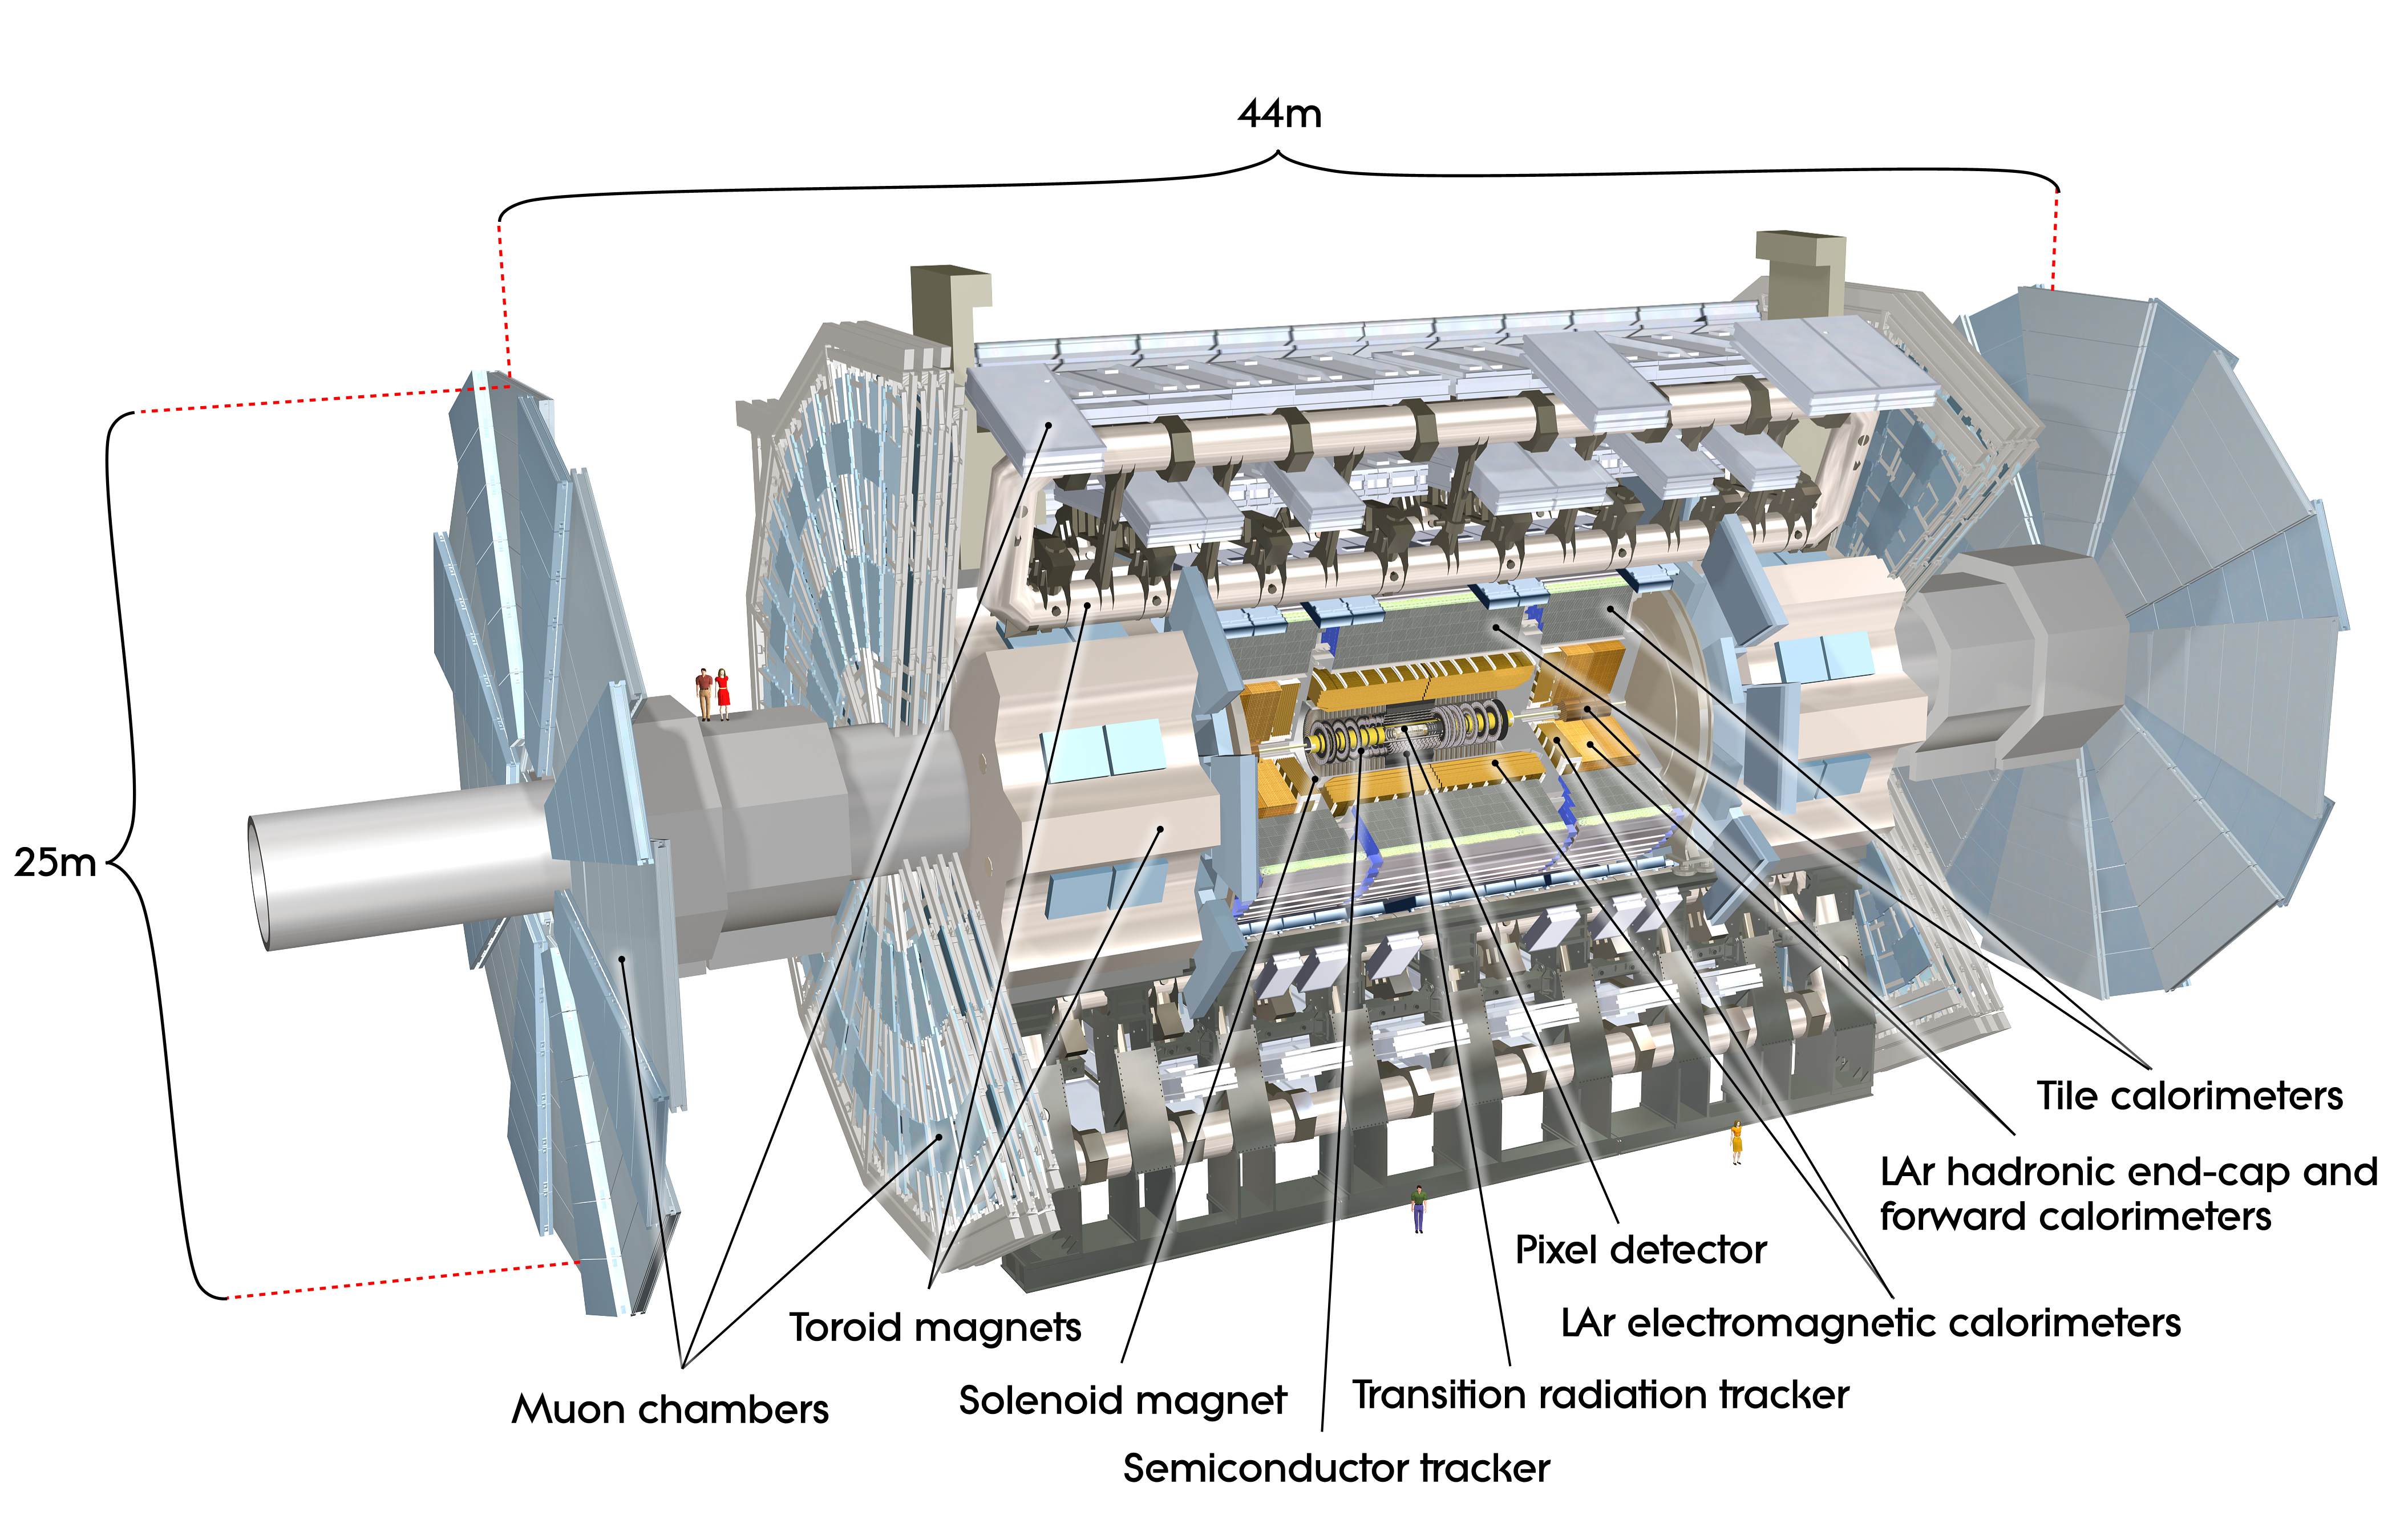
\includegraphics[width=0.9\textwidth]{figures/Detector/AtlasDetector.jpg}
  \caption[The ATLAS Detector]{
Schematic of the ATLAS detector.
Figure from \cite{ref:ATLASExp}.
}
\label{Det:ATLAS}
\end{figure}


\subsection{Detector Overview}
\label{sec:Det:Over}

A schematic of the ATLAS detector is shown in figure \ref{Det:ATLAS}. 
In this section the different detectors which make up the ATLAS detector will be reviewed. 
First the magnet system, which provides the magnetic field for the tracking detectors, will be discribed. 
Next the inner detector, the closest detector to the beam line, will be discribed, followed by the calorimeter systems and the muon detectors.

  %{sec:Det:Over}
\subsection{Magnet System}

The purpose of the magnet system in ATLAS is to bend charged particles, such that the tracking detectors can measure their transverse momentum using the curvature of the track. 
There are two different tracking regions, one very close to the interaction point which measures all charged particles, and then one tracking system at the outermost part of the detector which just measures the muon tracks. 
There is a different magnet system for each tracking region.
The magnet providing a field close to the interaction point is solenoidal, and provides a 2 T field for the inner detector. 
The system for the muon tracking has a set of toroidal magnets.
One set of barrel toroids combine with the two end-cap toroids to provide the muon tracking with a magnetic field of 0.5 T and 1 T, respectively.


\subsection{Inner Detector}
The inner detector (ID) provides full tracking information for $|\eta|<2.5$. 
The purpose of the ATLAS tracking detectors is to make high precision measurements of charged particle tracks near the beam line. 
These measurements are used for primary and secondary vertex finding and momentum determination. 
The tracking detectors have to be able to deal with the high track multiplicity expected at the design luminosity of the LHC.

\begin{figure}  
\centering  
\includegraphics[width=0.9\textwidth]{figures/Detector/AtlasID.jpg}
\caption[The ATLAS Inner Detector]{
A schematic of the ATLAS Inner Detector.
Figure from \cite{ref:ATLASExp}.
  \label{Det:ATLASID}
}
\end{figure}

Figure \ref{Det:ATLASID} shows the different components of the ATLAS inner detector that will be discussed. 
Both the pixel detector and the semiconducting tracker have a tracking region out to $|\eta|<2.5$, and the transition radiation tracker goes out to $|\eta|<2$. 

The pixel detector is the closest to the interaction point, and thus has the highest granularity of the inner detector trackers. 
There are three pixel layers in the barrel region each having a 2d segmentation, with a minimum size of $\phi\times z$ of $50\times400~\mu\rm{m}^2$, giving a well measured space point. 
The main use of the pixel detector is to find B hadrons and $\tau$ leptons. 

Further from the interaction point is the semi conductor tracker (SCT) which is less granulated. 
%*how does it work? 8 measurement from 4 layers + some detector pairs *. 
The main use of the SCT is determining track momenta, impact parameters and vertex positions.

Furthest away from the interaction point is the transition radiation tubes detector (TRT), which provides a large number of hits per track. 
The position accuracy of these hits is less accurate than that from the pixel and SCT detectors
The TRT was not used for tracking in 2010 data-taking.

\subsection{Calorimeter System}
\label{sec:Det:Calo}

The ATLAS calorimeter system, shown in Figure \ref{Det:ATLASCalo}, is a combination of different sampling detectors that are required to contain and measure both electromagnetic (EM) and hadronic showers over a large $|\eta|$ region. 
The main ATLAS calorimeter system consists of an EM calorimeter and a hadronic calorimeter, each of which aims to contain and measure EM and hadronic showers, respectively. 
There are also two forward calorimeters, one at each end of the experiment, at larger $\eta{}$, which measure both EM and hadronic energy deposits.
Different detector technology is used depending on the required accuracy for physics measurements and the radiation levels expected in different regions.
The amount of material, in radiation lengths, is shown in Figure \ref{Det:RadLegnth} for the different components of the ATLAS calorimeter system. 


\begin{figure}
  \centering
  \includegraphics[width=0.9\textwidth]{figures/Detector/AtlasCalorimeter.jpg}
\caption[The ATLAS Calorimeter System]{
Schematic of the ATLAS calorimeter system.
Figure from \cite{ref:ATLASExp}.
\label{Det:ATLASCalo}
}
\end{figure}

\begin{figure}
  \centering
  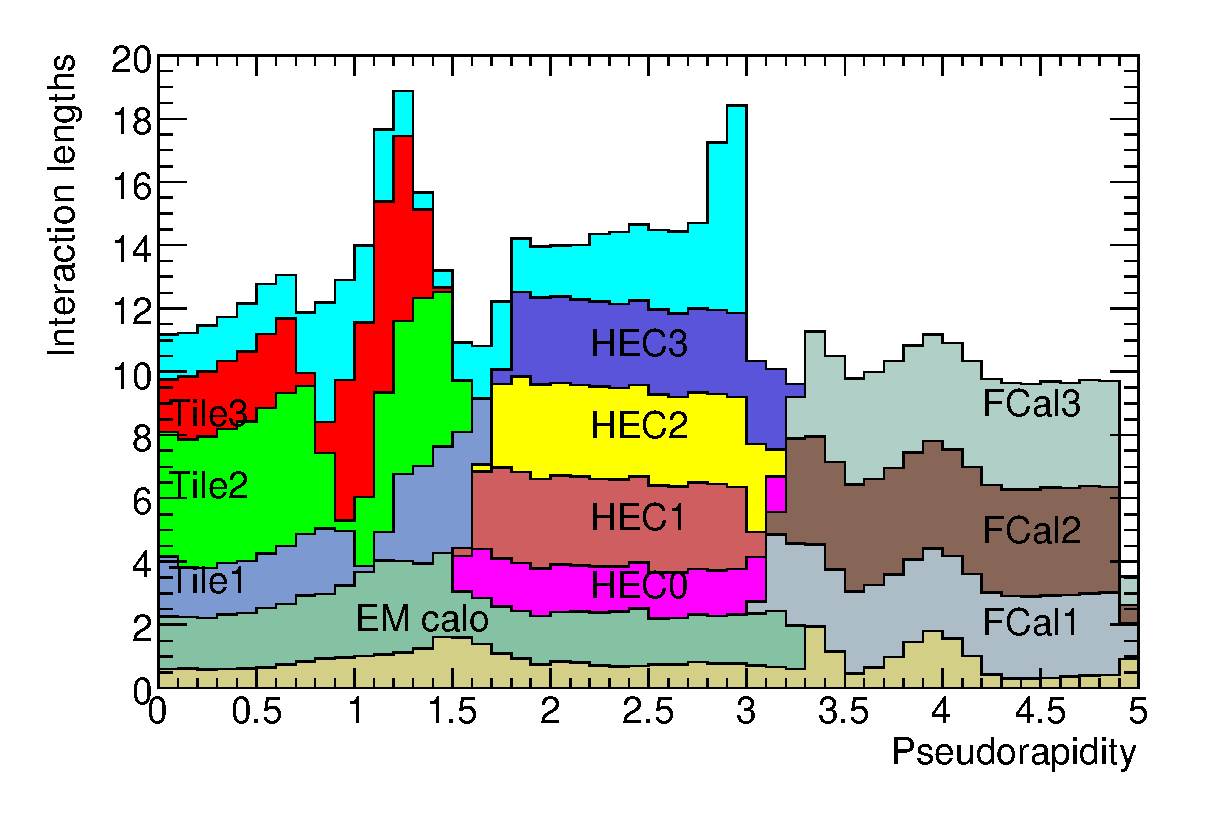
\includegraphics[width=0.9\textwidth]{figures/Detector/CalorimeterRadLegnths.eps}
  \caption[Radiation Lengths of the Calorimeter Sub-detectors ]{
Amount of material, in interaction lengths, in front of the different calorimeters.
The electromagnetic calorimeter is labelled ``EM calo'', the hadronic calorimeter is segmented into ``Tile'' and ``HEC'' layers, and the forward calorimeters is segmented with labels ``FCal''.
The final layer shown outermost for $|\eta|<3$ is the muon spectrometer.
Figure from \cite{ref:ATLASExp}.
\label{Det:RadLegnth}
}
\end{figure}





\subsubsection{EM Calorimeter}

The EM calorimeter is a sampling calorimeter with liquid argon (LAr) as the active material. 
It has complete azimuthal coverage for $|\eta|<3.2$ and is used to give precision measurements of EM showers.
Figure \ref{Det:ATLASCalo} shows the EM barrel and the EM end-cap, which have the pseudorapidity range $|\eta|<1.475$ and $1.375<|\eta|<3.2$, respectively.
In the precision region,  which is the region that overlaps the inner detector ($|\eta|<2.5$), there are three active layers and the detector is finely granulated to give a precise position measurement for the EM shower (used for photons).
Outside of the precision region there are two active layers and the granularity is coarser.
A presampler layer of LAr, which is in front of the first EM layer out to $|\eta|<1.8$, is used to correct for energy lost before the EM calorimeter. 
The EM calorimeter has greater than 22 radiation lengths to attempt to fully contain any EM showers.
The EM calorimeter cell information is calibrated to an EM scale using the decays of $Z$, $W$ and $\mathcal{J}/\psi$ as presented in \cite{ref:ZeeCalib}. 
The uncertainty on the electron EM scale is $<2\%$ for $|\eta|<2.7$ and $2-3\%$ for $2.5<|\eta|<4.9$. 

\subsubsection{Hadronic Calorimeter}



The hadronic calorimeter is situated behind the EM calorimeter covering the same $\eta$ region, and is responsible for the measurement of hadronic showers. 
It consists of three tile calorimeters (one barrel and two extended barrels) in the region $|\eta|<1.7$ and two hadronic end-caps (HEC) to extend the coverage to $|\eta|<3.2$ as shown in Figure \ref{Det:ATLASCalo}.
The hadronic calorimeter is a sampling detector, and the different components use different technologies with the tile calorimeter using  scintillating tiles as the active material and steel for the absorber, and the HECs using LAr as the active material and copper as the absorber.

The HEC has two wheels per end-cap, each with 32 wedged-shaped modules and has a granulation of $\Delta\eta~\rm{x}~\Delta\phi = 0.1~\rm{x}~0.1$ in the region $|\eta|<2.5$ and $\Delta\eta~\rm{x}~\Delta\phi = 0.2~\rm{x}~0.2$ in the region $2.5<|\eta|<3.2$.
Each wheel has two different depth segments, resulting in four layers per end-cap.

The tile calorimeter has three components, one barrel and two extended barrels.
The tile barrel and tile extended barrel cover the range $|\eta|<1$ and $0.8<|\eta|<1.7$ respectively.
These detectors comprise 64 modules which have a size of $\Delta\phi\approx0.1$, resulting in a granularity of $\Delta\eta~\rm{x}~\Delta\phi = 0.1~\rm{x}~0.1$.

\subsubsection{Forward Calorimeter}

The forward calorimeter (FCal), shown in Figure \ref{Det:ATLASCalo}, is responsible for measuring both the EM and hadronic showers in the region $3.2<|\eta|<4.9$.
The FCal has three detecting layers, the first layer is made of copper that is optimised for EM measurements and the following two are tungsten layers used to measure hadronic energy deposits.
All layers have LAr as the active material.
The choice of materials and design is largely determined by the need to be radiation hard to withstand the high particle flux.


\subsubsection{Calorimeter Objects}


To help construct offline physics objects, such as photons, electrons, taus or jets, an algorithm to cluster calorimeter readout cells is used.
The aim of clustering is to reconstruct the 3D EM or hadronic shower from the calorimeter cells.
Two clustering algorithms are used, the ``sliding window'' algorithm for photon, electron or tau identification, and the ``topological'' algorithm for jets.
The sliding window algorithm combines cell information from cells within a fixed size rectangular window in $\eta$ and $\phi$. 
Topological clusters, or ``topocluster'', are formed from a cluster seed, which is a cell with $|E|/\sigma_{noise}>4$, where $\sigma_{noise}$ is the expected noise in the calorimeter from the readout electronics and ``pile-up'' contributions. 
The cluster is then extended by including all cells next to it with $|E|/\sigma_{noise}>2$.
An additional layer of cells with $|E|/\sigma_{noise}>0$ are included.
The advantage of using this clustering rather than towers (groups of cells at fixed $\Delta\eta$ and $\Delta\phi$) is to improve noise suppression.
More information regarding topoclusters and sliding window clustering, and their performance, can be found in \cite{ref:ZeeCalib,ref:Clustering}.

%https://twiki.cern.ch/twiki/pub/Atlas/TapmJet/jetslice_v3_6April08.pdf


\subsection{Muon Detectors}

Furthest from the interaction point are the muon detectors. 
The muon detectors measure the hits from muons which are bent by the magnetic fields from the barrel toroid  and end-cap toroids, and a combination of both in the region between. 
The muon system has separate dedicated detectors for both precision position measurements and for triggering on muons.

For the precision measurement, Monitored Drift Tubes (MDT) are used in the rapidity range $|\eta|<2.7$, with the higher granularity Cathode Strip Chambers (CSC) used in the more forward region of $2<|\eta|<2.7$ in the innermost layer. 

The muon triggering system consists of Resistive Plate Chambers (RPC) in the barrel region and Thin Gap Chambers (TGC) in the end-cap region. 
The muon triggering system covers the region of $|\eta|<2.4$. 



\subsection{Trigger and Data Acquisition}
\label{sec:Det:Trig}
The event rate from the LHC is 1GHz *Check This*, but only $\mathcal{O}(200Hz)$ will be recorded to disk. 
The ATLAS trigger and data acquisition system (TDAQ) reduces the initial event rate by trying to select out the most interesting events.
TDAQ is split into subsystems that are approximately associated with the sub-detectors previously described. 
The three different trigger levels are level 1 (L1), level 2 (L2), and event filter (EF). 
The L2 and EF triggers are called the higher level triggers (HLT). 
The trigger levels are applied in series, with each level refining the decision and adding additional requirements. 
L1 is required to make a decision in less than $2.5\mu$s and reduce the rate to 75 kHz. 
If the event has passed a L1 trigger, it then goes through the L2 and EF trigger which have more information about the event and reduce the rate to 200Hz.
While the trigger is deciding if the event should be kept, the data acquisition system is buffering the event information.


L1 triggers try and select interesting objects, such as high $p_T$ jets, electrons, muons, photons, taus or large missing $E_T$, which are indicative of interesting physics processes. 
The main three detector systems that trigger events at the L1 level are the RPC and TGC, which trigger on muons, the calorimeter with reduced granularity, which triggers on the jets, electrons, muons, photons, or large missing $E_T$, and the Minimum Bias triggers that trigger on minimal energy and used to select an unbiased sample of events. 
The results from the muon, calorimeter and minimum bias triggers are passed to the central trigger process. 
This then applies a trigger menu, which is list of triggers, their thresholds and prescales. 
By applying a prescale, $p$, to a trigger, only $\frac{1}{p}$ of the events that fired the trigger will be passed to L2. 
The purpose of the prescale is to reduce the rate of less interesting or high rate processes and also to keep the overall rate constant as the luminosity changes.
If the event fires the L1 trigger and passes the prescale, the L1 trigger passes the region of interest, ROI, (this is a $\eta\phi$ region near the triggered object) to the HLT.
The L2 triggers have access to the full granularity around the L1 ROI, but cannot do full reconstruction in the 40 ns given to make the initial decision. 
With the extra time, more information is used to make tighter and additional cuts to reduce the rate to 3.5 kHz.
The EF triggers have approximately four seconds to make a decision.
This is long enough to do longer offline analysis procedures which help to reduce the overall rate written to disk to 200 Hz.

The important triggers for this thesis are the calorimeter trigger (specifically the jet trigger) and the minimum bias trigger, which will be discussed below.

\subsubsection{Minimum Bias Triggers}
The minimum bias triggers aim to provide a trigger that is not biased towards any particular physics process or to high $p_T$ objects. 
This is achieved by having a set of minimum bias trigger scintillator counters (MBTS) at the front of the calorimeter endcaps ($2<|\eta|<3.8$). 
This is easily fired by having a low energy hit threshold. 
The result is a very high rate from the MBTS, such that it is heavily prescaled for all but the lowest luminosity runs. 
The MBTS is ideal to check the bias of trigger strategies. 



\subsubsection{L1 Calorimeter}
The L1 calorimeter trigger (L1Calo) is the trigger system concerned with both the EM calorimeter and the hadronic calorimeter. 
The EM and Had calorimeter readout cells are merged into trigger towers of $\Delta\eta \rm{x} \Delta\phi$ of 0.1 x 0.1 for the precision region and increasing size for regions of higher rapidity. 
Trigger towers are used to define jet, electron, photon and tau trigger objects.

\subsubsection{Jet Triggers}

L1 jet trigger objects are found by first defining jet elements from 2x2 trigger towers in both the EM and hadronic calorimeters.
In the central precision region the jet elements cover a region of $\Delta\eta \rm{x} \Delta\Phi = 0.2\rm{x}0.2$. 
A sliding window algorithm is used to find the L1 jet objects. 
The algorithm can be set have a window of either 2x3, 3x3 or 4x4 jet elements for the jet finding, and it looks over the jet elements to find local maxima in \et{} which are greater than a given threshold. 
The L1 jet triggers are named L1\_JX where X is the EM energy threshold for the jet object.

Once the L1 jets are found the ROIs, regions of interest (positions of jets), are passed to the HLT, and act as seeds. 
The L2 jet trigger can access the course calorimeter information within a tuneable (*what is the default*) $\Delta\eta\Delta\phi$ around the L1 jet ROI. 
This information is then passed into a seeded cone jet algorithm (see section XXX), which is a basic and fast jet finder which uses jet radius, R, of 0.4, and which is restricted to three iterations.
The L2 can access finer calorimeter information and produce cone-like jets.
The hadronic components of the jet at L2 had been calibrated.
This is important as the have a lower response to energy deposits than the EM components. 

%https://twiki.cern.ch/twiki/pub/Atlas/TapmJet/jetslice_v3_6April08.pdf


 
\section{Jets in ATLAS}
\label{sec:Det:Jets}

The jet definition within ATLAS uses the \antikt{} algorithm, which is described in Section \ref{sec:Theory:Jets}. 
This algorithm groups related energy deposits in the ATLAS calorimeters.
Different input objects can be used with the \antikt{} algorithm, such as cells, towers and topoclusters and these objects can be calibrated to different energy scales.
In this analysis, unless otherwise stated, the jets are defined using the \antikt{} algorithm with a distance parameter of 0.6 running over topocluster at EM scale, where topoclusters and EM scale are defined in Section \ref{sec:Det:Calo}.


\subsubsection{Jet Energy Scale (JES)}

The jet response needs to be calibrated to take into account both detector and physics responses such as dead material, particle being bent into and  out of the jet, and noise threshold variation. 
Also, jets are found using EM-scale topoclusters and need to be calibrated due to the non-compensation of the hadronic calorimeter which has a lower detector response to hadrons than to EM deposits.
An EM+JES calibration was determined as a function of the jet \pt{} and rapidity to account for these effects.

The EM+JES calibration was done in three consecutive corrections.
The first was a pile-up offset correction designed to subtract energy contributions due to additional $pp$ interactions.
The correction is presented in \cite{ref:OffsetCorrection}, where the average energy in towers is considered as a function of the rapidity, the number of primary vertices and the bunch spacing.
The second correction was the vertex correction, which defined the origin of the jets to be the primary vertex.
This correction changes the direction and \pt{} of the jet, but not the energy, and it improves the angular resolution of the jet.
The final correction is the jet energy scale (JES) correction.

The JES correction uses fully simulated MC, ``reco'', jets and jets at hadron level, ``truth'' jets, to obtain correction factors as a function of jet energy and jet rapidity. 
The response of the calorimeter to jets can be defined using these fully simulated MC samples as
\begin{equation}
\mathcal{R(\eta)} = \frac{\pt{}^{reco}(\eta)}{\pt{}^{truth}(\eta)}
\label{JetPerf:MCJetResp}
\end{equation}
where \pt{}$^{reco}$ is the \pt{} of the MC jet after full simulation of the detector, and  \pt{}$^{truth}$ is the \pt{} of the MC jet at hadron level.
The truth and reco jets are matched using a \dr{} cut of 0.3.
The correction factors are calculated as a function of the jet's detector $\eta$ (not the vertex corrected $\eta$), as they represent calibrations for different detectors, and also as a function of the energy, as the detector responds to energy. 
Figure \ref{Det:MCResp} shows the jet responses, at EM scale, as a function of detector $|\eta|$ for different jet energies. 
From the comparison between fully simulated MC jets and truth jets, a small correction on the jet rapidity is calculated. 
This is due to part of jets falling into regions with poor response, giving a rapidity bias towards the better responding areas. 

\begin{figure}
\centering
\mbox{
              %\epsfig{figure=figures/JetPerformance/MCResponse-ref_ATLAS-CONF-2010-055.eps,width=\textwidth}
              \epsfig{figure=figures/Detector/JetCalibfig_JES_vs_eta_Binning.eps,width=\textwidth}

                              }
\caption[Jet response for different regions of the ATLAS calorimeter]{ 
PYTHIA simulated jet EM-scale response as a function of reconstructed jet $\eta$ for different jet energies \cite{ref:JES}.
The different evaluated regions are shown, as well as their relation to the detector geometry. 
\label{Det:MCResp}
}
\end{figure}

The original derivation of these factors can be found in \cite{ref:OffsetCorrection,ref:JES_basic,ref:JES}.

\subsubsection{Jet Energy Scale Uncertainty}

The EM+JES method of calibration is based primarily on the ability of the MC to correctly simulate the ATLAS detector and also to model the physics effects such as energy flow out of the jet.
In-situ methods are used to validate the JES calibration and assign an uncertainty.
The JES uncertainty is derived from in-situ data measurements and also by varying MC settings. 
It is determined by combining the non-closure of the EM+JES on fully simulated MC jets, calorimeter response to isolated hadrons using test-beam information and in-situ methods, additional detector material, noise thresholds, differences compared to other MC's, uncertainties due to pile-up and \pt{} balance of dijet events. 


\begin{figure}
\centering
\mbox{
              \epsfig{figure=figures/Detector/JESSummary_JESUncertainty_AntiKt6Topo_EMJES2.1-2.8.eps,width=0.8\textwidth}

                              }
\caption[JES Uncertainty]{ 
Fractional JES uncertainty for jets with $2.1\le|\eta|\le2.8$ as a function of the jet \pt{} \cite{ref:JES}. 
\label{Det:JESU}
}
\end{figure}

Figure \ref{Det:JESU} shows the fractional JES uncertainty for jets with $2.1\le|\eta|\le2.8$ as a function of the jet \pt{}.
The dominant systematic at high \pt{} is the single particle response which comes from test-beam single pion information and the calorimeter response for a single hadron.
At low \pt{}, dijet balance (intercalibration) is the most significant uncertainty.
Dijet balance is an in-situ method of extending the uncertainty in the central region to other regions of the detector, and will be discussed in more detail in Chapter \ref{chp:JetPerf}.


\subsubsection{Jet Energy Resolution}

The jet energy resolution (JER) is a measure of the expected range of measured jet \pt{} compared to the original object. 
Some causes of the fluctuations in the measurement of a jet \pt{} are hadron/EM contributions, non-average amount of additional energy from pile-up, and statistical fluctuations in the sampling technique across multiple calorimeter layers.
The JER was determined using the bi-sector method and the \pt{} balance of dijet events described in \cite{ref:JER,ref:JER2}. 




\subsubsection{Jet Cleaning}

Jets produced in an event need to be discriminated from ``bad'' background jets that come from  HEC spikes and EM noise in the calorimeter, cosmic rays or non-collision background.
Table \ref{det:Cleaning} shows the loose and medium cleaning cuts used to remove the bad jets where
\begin{itemize}
  \item The jet charge fraction, \Bold{Chf}, is the ratio of the sum of the \pt{} of tracks associated to the jet to the calibrated jet \pt{};
  \item \Bold{EMf} is the fraction of the jet EM scale energy that comes from EM clusters;
  \item \Bold{HECf} is the fraction of the jet energy that was measured in the HEC;
  \item The LAr quality, \Bold{LArQ}, is the fraction of the jet energy coming from LAr cells with poor signal shape quality;
  \item The HEC quality, \Bold{HECQ}, is the fraction of the jet energy coming from HEC cells with poor signal shape quality;
  \item \Bold{neg. E} is the sum of the negative energy cells in the jet;
  \item Jet time, \Bold{t}, is the mean time between the cells in the jet and the event time;
  \item \Bold{FMax} is the maximum energy fraction in one calorimeter layer.
\end{itemize}

Jets coming from HEC spikes have most of the energy coming from a single noisy calorimeter cell, and so a HECf cut is applied to ensure energy deposits outside the HEC form a significant part of the total energy.
Fake jets coming from EM coherent noise are removed by cutting on the fraction of EM energy.
Finally, jets from non-collision backgrounds and cosmics are removed using a combination of timing cuts and energy layer cuts.

The loose cleaning cuts are defined to have an efficiency of greater than 99\% for good jets, but a fraction of bad jets still remain. 
Whilst, the medium cleaning cuts remove a higher proportion of bad jets, they have inefficiencies at low \pt{} for good jets. 

While the bad jets do not come from energy deposits from the interaction, there is a subset of jets, called ``ugly'' jets, which are energy deposits from the interaction which have been badly measured. 
Ugly jets are often found in regions between detectors, ``cracks'' regions, where the performance of the detectors are not optimal.
Two cuts are applied to remove ugly jets.
First, the jet energy which falls into the transition between the barrel and the end-cap is required to be less that half the total jet energy.
Second, the fraction of energy that comes from bad cells inside the jet is required to be less than half of the total energy.


\begin{table}
\begin{center}
\footnotesize

\begin{tabular}{|c||c|c|}
\hline
& Loose & Medium = Loose OR \\
\hline
            & $\rm HECf<0.5$ \& $|\rm HECQ|>0.5$                         &                                                              \\
HEC spikes  &              or                                              & $\rm HECf>1-|HECQ|$                                          \\
            &  $\rm |neg.E|>60$ GeV                                        &                                                              \\
\hline
EM          &                                                              &                                                              \\
coherent    & $\rm EMf >0.95$ \& $\rm |LArQ| >0.8$ \& $|\eta|<2.8$     &   $\rm EMf >0.9$ \& $\rm |LArQ| >0.8$ \& $|\eta|<2.8$    \\
noise       &                                                              &                                                              \\
\hline
            &           $\rm |t|>25$ ns                                                    &                                                              \\
Non-        &              or                                              &  $\rm |t|>10$ ns                                          \\
collision   & $\rm EMf <0.05$ \& $\rm Chf<0.05$ \& $|\eta|<2$     &   or     \\
background  &        or                     &   $\rm EMf<0.05$ \& $\rm Chf <0.1$ \& $|\eta|<2$    \\
\& cosmics  & $\rm EMf <0.05$ \&  $|\eta|>2$     &   or     \\
            &        or                     &   $\rm EMf>0.95$ \& $\rm Chf <0.05$ \& $|\eta|<2$    \\
             & $\rm FMax<0.99$ \&  $|\eta|<2$     &        \\

\hline

\end{tabular}
\caption[Jet Cleaning Definitions]{
Loose and Medium jet cleaning definitions.
\label{det:Cleaning}
}
\end{center}
\end{table}


 

\chapter{High Level Trigger Calorimeter Monitoring}
\label{chp:HLTCalo}
The calorimeter high-level trigger (HLTCalo) is used to trigger on physics objects that deposit their energy in either the electromagnetic or hadronic calorimeter.
As described in Section \ref{sec:Det:Calo}, the calorimeter is segmented into cells.
These cells are clustered together and can be combined with inner detector tracks to define physics objects such as electrons, photons, taus, and jets. 

The HLTCalo is monitored to check the performance and consistency of the triggers. 
This is achieved by monitoring the individual cells in the calorimeters and also by comparing the different L2 and EF triggered physics objects to the corresponding offline object.
Flags are defined for each monitoring distribution, where a green flag represents the distribution is consistent with the expected distribution, and yellow and red represent a deviation from the expected distribution. 
When the flag is red or yellow the distribution is studied further via a web based graphical user interface to find the reason, and if necessary the associated data can then be excluded from physics analysis.


In this chapter, work done by the author on improvements to the current cell monitoring which expose hot cells, and the addition of monitoring of calorimeter objects are discussed. 

\section{Cells}

The overall HLTCalo monitoring is done on a cell by cell basis.
This monitoring consists of distributions showing the number of active cells in the LAr and Tile calorimeters, the number of problematic cells and the position of these cells in the LAr and Tile calorimeters, and also the difference in cell energy between the trigger levels and offline levels.

The number of cells in the LAr and Tile calorimeters is an example of a monitoring plot that is very stable and should only change when a hot cell is masked or taken offline, allowing very tight flag definitions.
Monitoring plots, such as the percentage difference in energy in the trigger and offline cells, vary significantly ($\approx15\%$) with different running conditions, so either looser or no flag definitions are set.

The average transverse energy per cell in $\eta  \phi$ distribution is important in identifying hot spots where one cell records artificially high energy in every event.
Hot cells can be caused from electronic problems within the cells. 
Figure \ref{SW_hotspot} shows an example of a hot spot found using the offline cell monitoring in run 201191. 
This resulted in the cell being masked.

\begin{figure}
\centering
\mbox{
   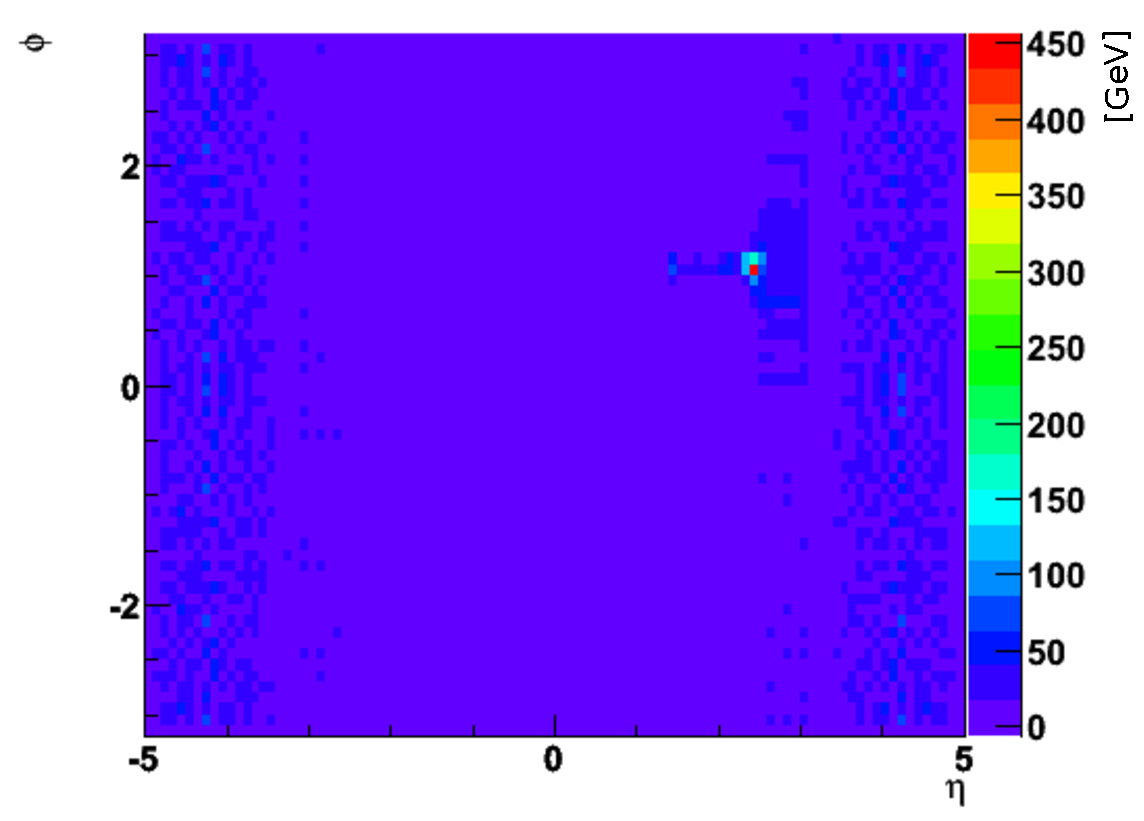
\includegraphics[width=0.9\textwidth]{figures/ServiceWork/Cells_HotSpot-Edit.pdf}
}
\caption[Average \et{} for HLT calorimeter cells]{
Average \et{} per $\eta \phi$ bin in run 201191. 
A hot region is observed at $\eta=2.5$ $\phi=1$. 
\label{SW_hotspot}}
\end{figure}



\section{Calorimeter Objects}

The HLTCalo is also monitored by comparing calorimeter triggered objects (electrons, photons and jets) to the offline objects.
A cut on the \dr{} is made to match the triggered objects to the offline objects.
An \et{} cut has been applied to the offline objects, which is the same as required by the analysis selection. 



\subsection{Electrons and Photons}



%-Define the offline and two trigger clusters
%-explain difference between two trigger level clusters
%-Show the matching cuts
%-Explain the reason for the plots
%-For the plot, make sure we explain the red points.

The EM calorimeter component of the HLTCalo is monitored by using physics objects that are reconstructed using EM energy deposits from electrons and photons. 
There are differences between the L2 and EF level EM cluster finding due to the time constraints on the L2 trigger.  
The L2 EM clusters are found using only the second EM calorimeter layer, in which the highest energy cell is used as the cluster seed.
From this cluster seed, the cluster position is formed using the energy weighted $\eta$ $\phi$ from a grid of \etaphiB{0.075} around the seed, and the cluster energy is calculated by summing over the energy of the cells. 
Conversely, the EF EM clusters use a sliding-window cluster algorithm using the calorimeter towers. 
This reduces the effect of the hot cells, as these will be smeared by the surrounding regular cells which will not have energy deposits.
The offline clusters are also found using a sliding-window algorithm, but they have full offline cell information.
 

\subsubsection{EM cluster matching}

Matching the offline and trigger objects is done using \dr{}.
Figure \ref{SW_egamma_L2_dR} shows the \dr{} distribution between the offline and all L2 EM clusters.
Two peaks can be seen in (a), one at $\dr{}=0$ which corresponds to good matching.
Events often have two objects that will be back-to-back in \dphi{}, which corresponds to the peak at $\dr{}\approx\pi$. 
The peak at $\dr{}=0$ shown in the expanded view (b), which shows a minimum in the range \dr{} from 0.03 to 0.1.

Figure \ref{SW_egamma_EF_dR} shows the \dr{} distribution between the offline and all EF EM clusters.
As observed for the L2 \dr{} distribution, there are two peaks; one at $\dr{}=0$ and one at $\dr{}\approx\pi$. 
The minimum observed in (b) is in the range \dr{} from 0.02 to 0.1.

A \dr{} matching cut of 0.035 is used between the offline and both L2 and EF triggers as this selects the majority of the correctly matched clusters and is also the distance from the centre to the edge of the L2 cluster.
In addition, the offline cluster is required to have $\et{}>10$ GeV.  

\begin{figure}
\centering
        \begin{subfigure}[b]{0.5\textwidth}
                \centering
                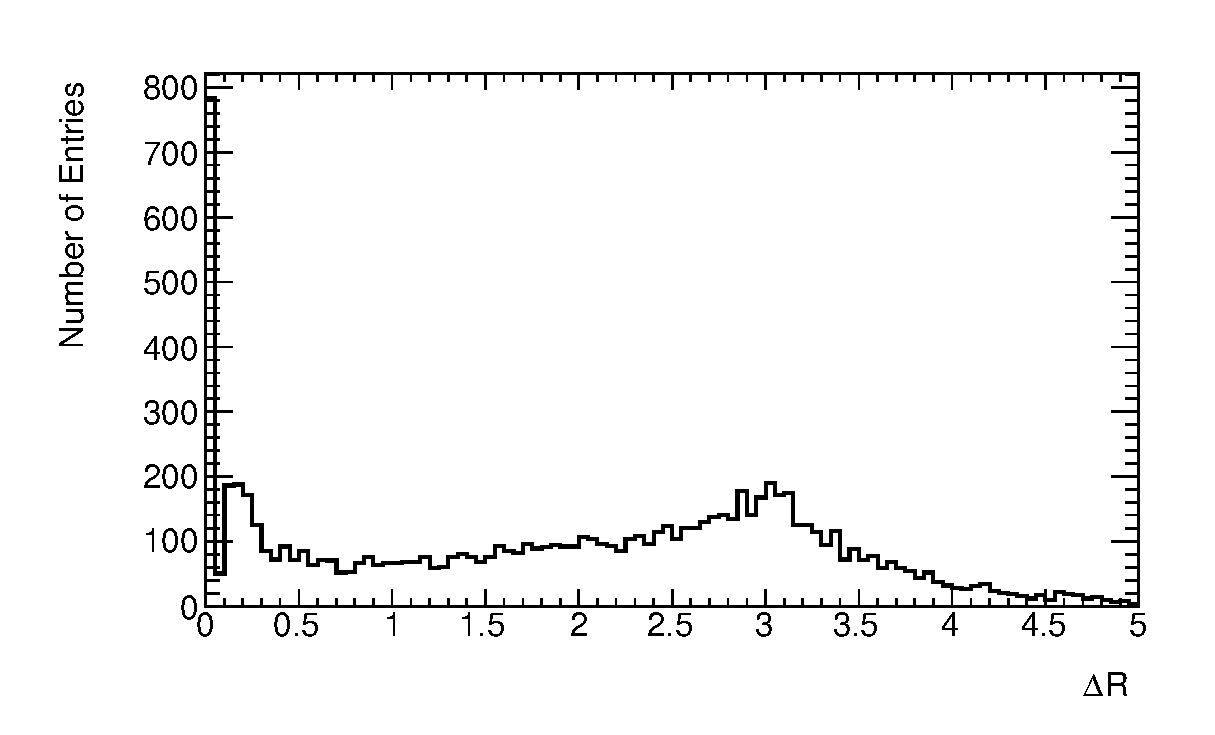
\includegraphics[width=\textwidth]{figures/ServiceWork/EgammaL2/DR_Unmatched_L2.eps}
        \end{subfigure}%
        \begin{subfigure}[b]{0.5\textwidth}
                \centering
                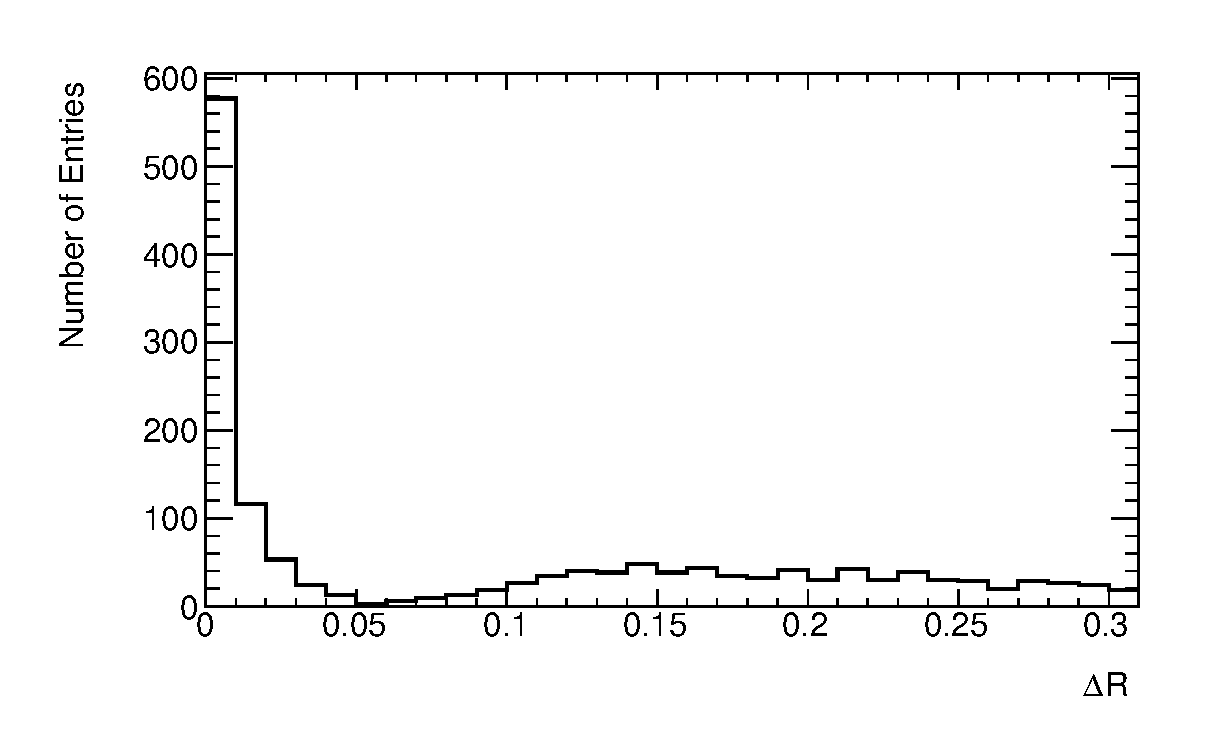
\includegraphics[width=\textwidth]{figures/ServiceWork/EgammaL2/DR_Unmatched_Zoomed_L2.eps}
        \end{subfigure}%
\caption[\dr{} between offline and L2 EM object]{
\dr{} distribution between the offline EM cluster and all L2 clusters in the event, shown within the range (a) $0 - 5$ and (b) $0 - 0.3$. 
\label{SW_egamma_L2_dR}}
\medskip
        \begin{subfigure}[b]{0.5\textwidth}
                \centering
                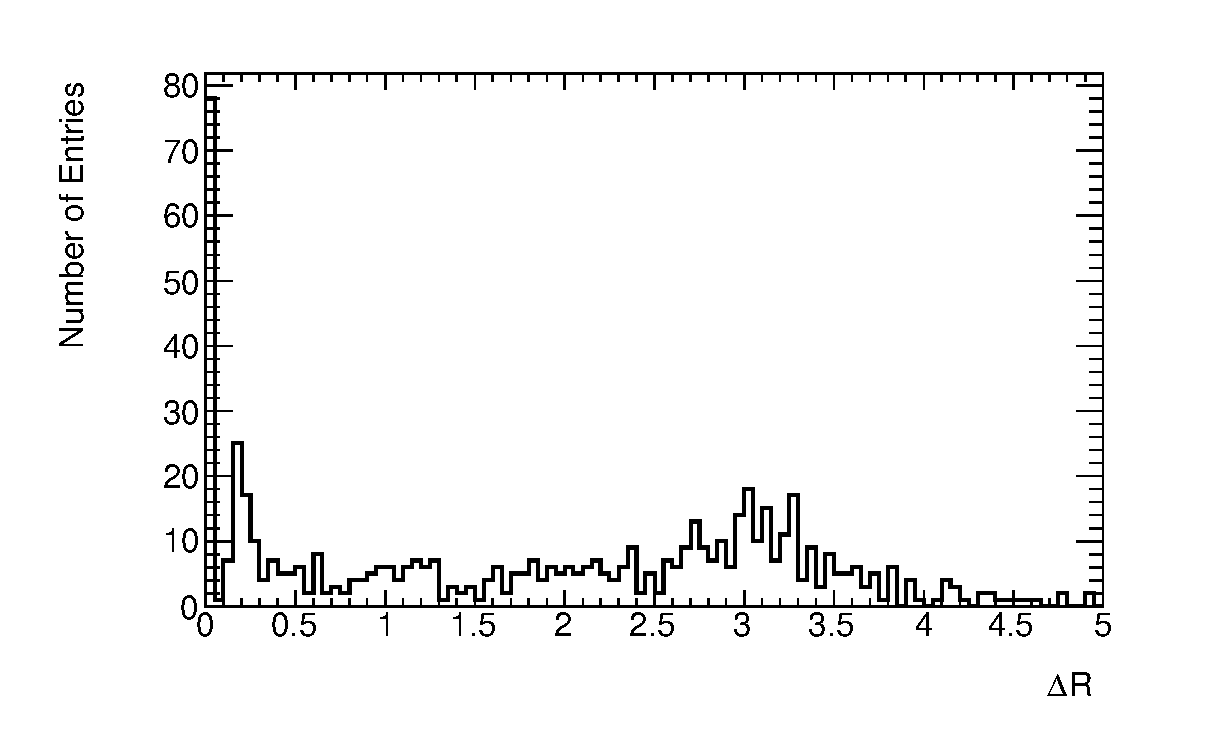
\includegraphics[width=\textwidth]{figures/ServiceWork/EgammaEF/DR_Unmatched_EF.eps}
        \end{subfigure}%
        \begin{subfigure}[b]{0.5\textwidth}
                \centering
                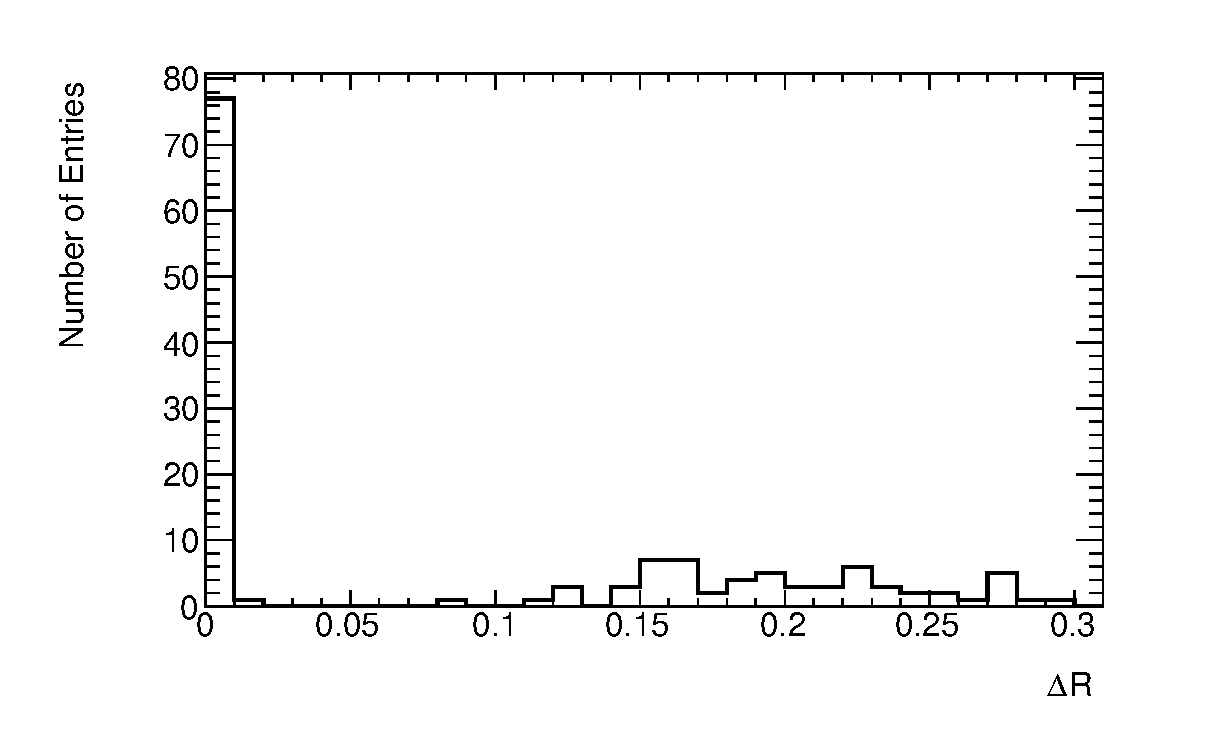
\includegraphics[width=\textwidth]{figures/ServiceWork/EgammaEF/DR_Unmatched_Zoomed_EF.eps}
        \end{subfigure}%
\caption[\dr{} between offline and EF EM object]{
\dr{} distribution between the offline EM cluster and all EF clusters in the event, shown within the range (a) $0 - 5$ and (b) $0 - 0.3$. 
\label{SW_egamma_EF_dR}}
\end{figure}




\subsubsection{Monitored Distributions}


The monitoring plots shown in Figures \ref{SW_egamma_L2EF_EtEt} -\ref{SW_egamma_L2EF_Reso} are from run 190644 in the  2011 data-taking.
Figure \ref{SW_egamma_L2EF_EtEt} shows the distribution of the offline EM cluster \et{} versus that of (a) a L2 and (b) a EF EM cluster \et{}.
This is useful in checking the linearity of the trigger EM clusters to the offline. 
The L2 EM cluster \et{} shows good linearity to the offline EM cluster \et{}, and the majority of events fall on a straight line where the \et{} of the offline and L2 are the same.
There is a significant band either side of this straight line, with more falling above the line.
This corresponds to a larger offline \et{} than L2 EM cluster \et{}.
The EF EM cluster \et{} has an even better linearity, and again most of events fall on a straight line corresponding to the offline EF clusters having the same \et{}.
The band around the events falling on the straight line is significantly smaller than for the L2 EM clusters.


Figure \ref{SW_egamma_L2EF_EtFrac} shows the distribution of \et{} fraction,
\begin{equation}
f(\et{})_{Trigger}=\frac{\et{}(\rm{Triggered~EM~cluster})}{\et{}(\rm{Offline~EM~cluster})},
\label{SW:EtFrac}
\end{equation}
as a function of $\eta{}$ for (a) the L2 EM clusters and (b) the EF EM clusters.
The \et{} fraction for the L2 EM clusters is centred around one, with most events within $5\%$.
The EF EM clusters' \et{} fraction is also centred around one, but with significantly smaller fluctuations.
In both distributions there is a region at $|\eta{}|=1.5$ where the fluctuations in the ratio from unity are larger.
This is due to the EM deposit falling into the crack region between the EM calorimeter barrel and the EM barrel end-cap.
There is an improvement in the EF due to the additional calibration done at EF level. 

Figure \ref{SW_egamma_L2EF_Reso} shows the distribution of the \et{} resolution,
\begin{equation}
\sigma(\et{}) =\frac{\et{}(\rm{Triggered~EM~cluster})-\et{}(\rm{Offline~EM~cluster})}{\et{}(\rm{Offline~EM~cluster})},
\label{SW:EtReso}
\end{equation}
for (a) L2 EM clusters and (b) EF EM clusters.
Both distributions have a mean $\sigma(\et{})$ of $<1\%$. 
The L2 EM cluster $\sigma(\et{})$ distribution has a larger spread than that for the EF.


All the monitoring distributions are susceptible to changes in calibration or the cluster sizes. 
The monitoring flags can be set to compare the mean of the distribution to the expected value.
The distributions in Figures \ref{SW_egamma_L2EF_EtFrac} and \ref{SW_egamma_L2EF_Reso} have flags set based on the mean of the \et{} fraction and $\sigma(\et{})$, respectively. 
If these show sizable differences from the expected mean, the distribution will be yellow or red flagged automatically.
Figure \ref{SW_egamma_L2EF_EtEt} can then be used to study the reason for the differences.

 
\begin{figure}
\centering
        \begin{subfigure}[b]{0.5\textwidth}
                \centering
                \includegraphics[width=\textwidth]{figures/ServiceWork/run_190644/EtEt_Matched_L2.eps}
        \end{subfigure}%
        \begin{subfigure}[b]{0.5\textwidth}
                \centering
                \includegraphics[width=\textwidth]{figures/ServiceWork/run_190644/EtEt_Matched_EF.eps}
        \end{subfigure}%
\caption[Offline EM \et{} versus L2 and EF EM \et{}]{
\et{} of the offline EM cluster versus the \et{} of the closest matched (a) L2 and (b) EF EM cluster.
\label{SW_egamma_L2EF_EtEt}}
\end{figure}

\begin{figure}
\centering
        \begin{subfigure}[b]{0.5\textwidth}
                \centering
                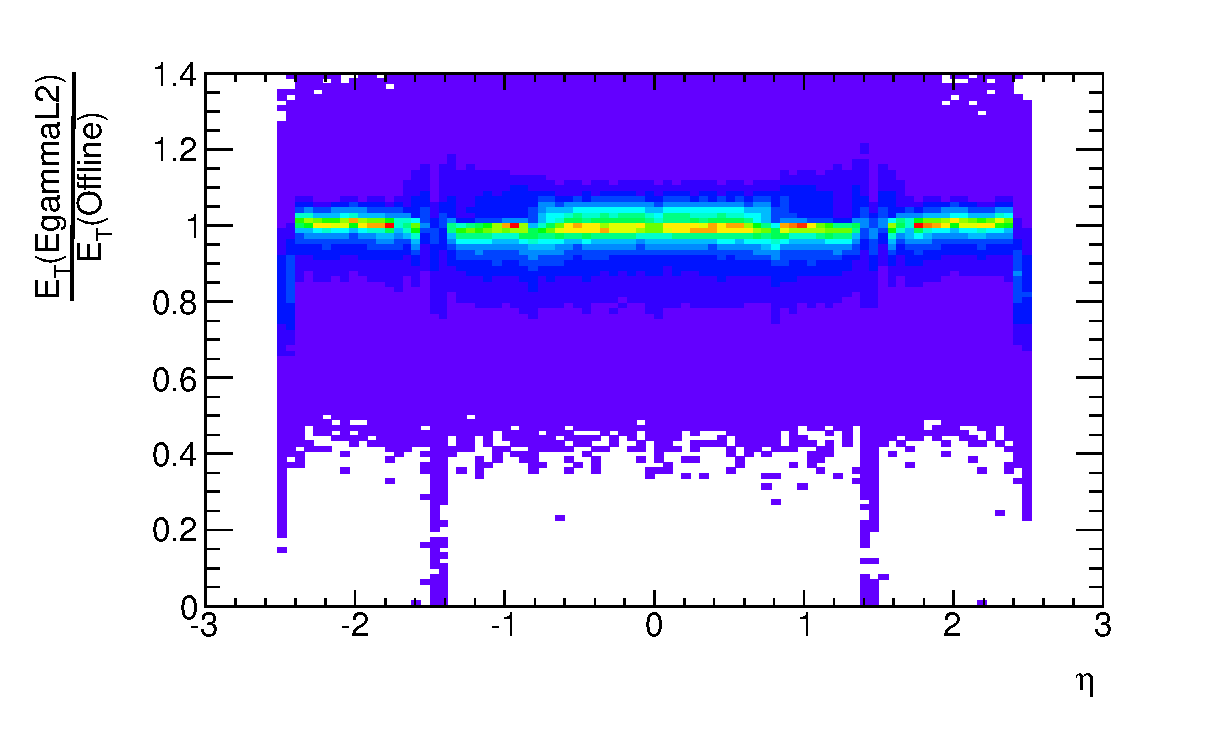
\includegraphics[width=\textwidth]{figures/ServiceWork/run_190644/EtFrac_Eta_Matched_L2.eps}
        \end{subfigure}%
        \begin{subfigure}[b]{0.5\textwidth}
                \centering
                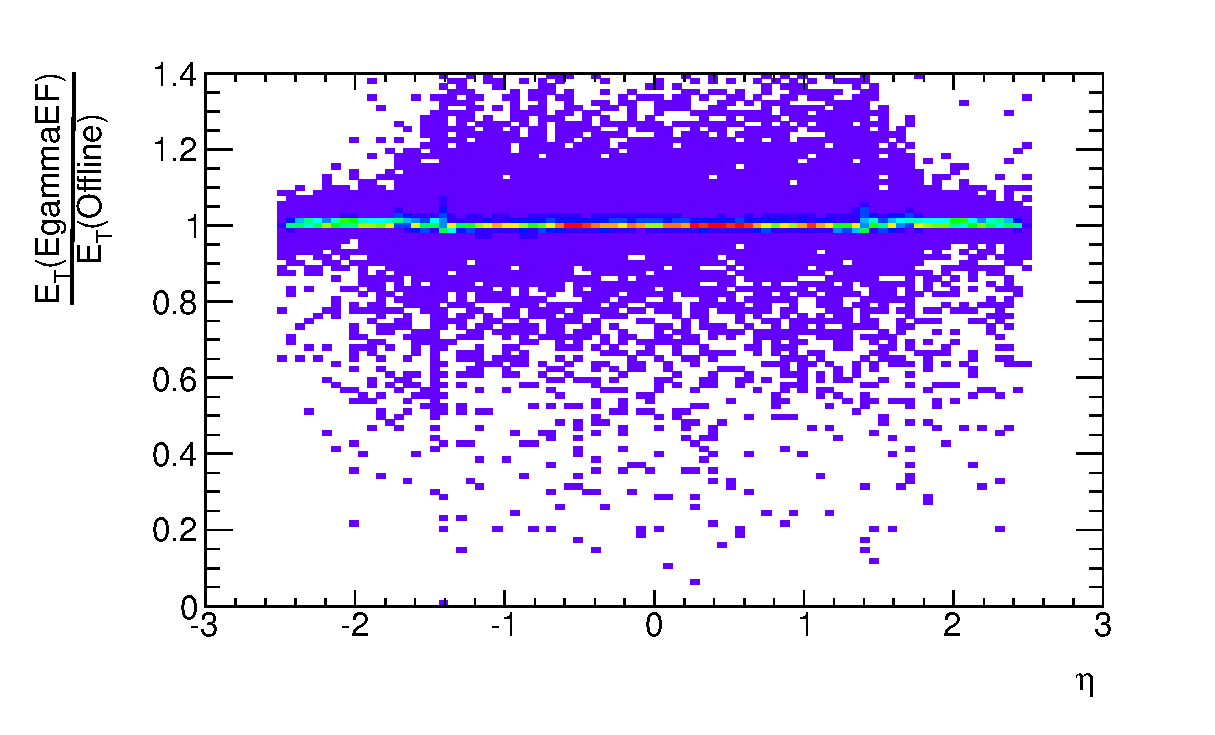
\includegraphics[width=\textwidth]{figures/ServiceWork/run_190644/EtFrac_Eta_Matched_EF.eps}
        \end{subfigure}%
\caption[\et{} fraction of L2 and EF to offline EM objects]{
\et{} fraction of (a) the  L2 and (b) the EF EM cluster  to the offline EM cluster \et{} as a function of $\eta$. 
\label{SW_egamma_L2EF_EtFrac}}
\end{figure}

\begin{figure}
\centering
        \begin{subfigure}[b]{0.5\textwidth}
                \centering
                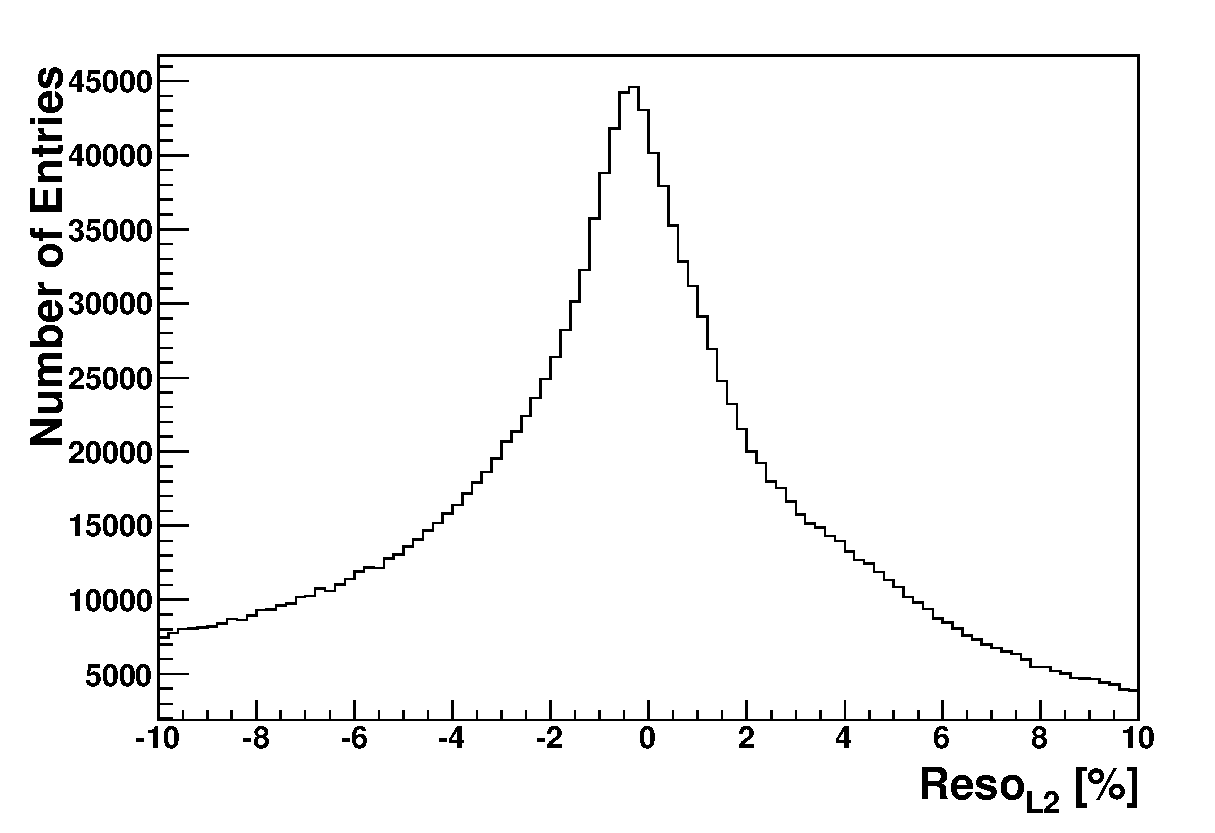
\includegraphics[width=\textwidth]{figures/ServiceWork/run_190644/Reso_Matched_L2.eps}
        \end{subfigure}%
        \begin{subfigure}[b]{0.5\textwidth}
                \centering
                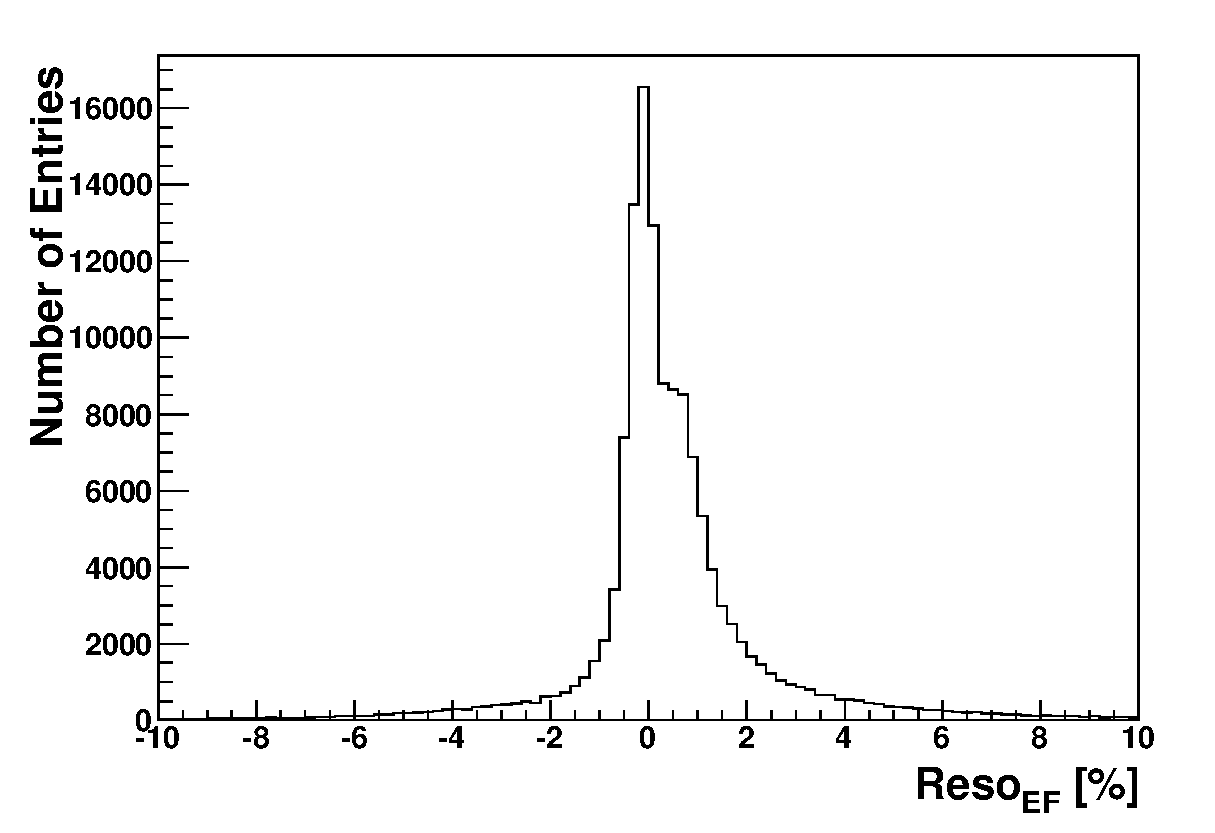
\includegraphics[width=\textwidth]{figures/ServiceWork/run_190644/Reso_Matched_EF.eps}
        \end{subfigure}%
\caption[Offline EM \et{} versus L2/EF EM \et{}]{
Distribution of the relative difference between the \et{} of the (a) L2 and (b) EF EM cluster, and the offline EM cluster \et{}.
\label{SW_egamma_L2EF_Reso}}
\end{figure}


Figure \ref{SW_egamma_EF_Reso_Range} shows the history of the mean of $\sigma(\et{})$ for EF EM clusters.
The colours of the points show the flag that was set for these runs.
Flags were assigned for a given run depending on the difference of the mean to a standard mean of $0.975\%$. 
The run is flagged green if the difference is less than $0.2\%$, yellow if between $0.2\% - 0.4\%$ or red if greater than $0.4\%$.
These flag values were tuned using the initial runs in the first data taking region.
Most of the runs are set as green or yellow, with only a few set as red.
The red flagged runs are those where there is no stable beam and some sections of the LAr calorimeter were not online during the run.


\begin{figure}
\centering
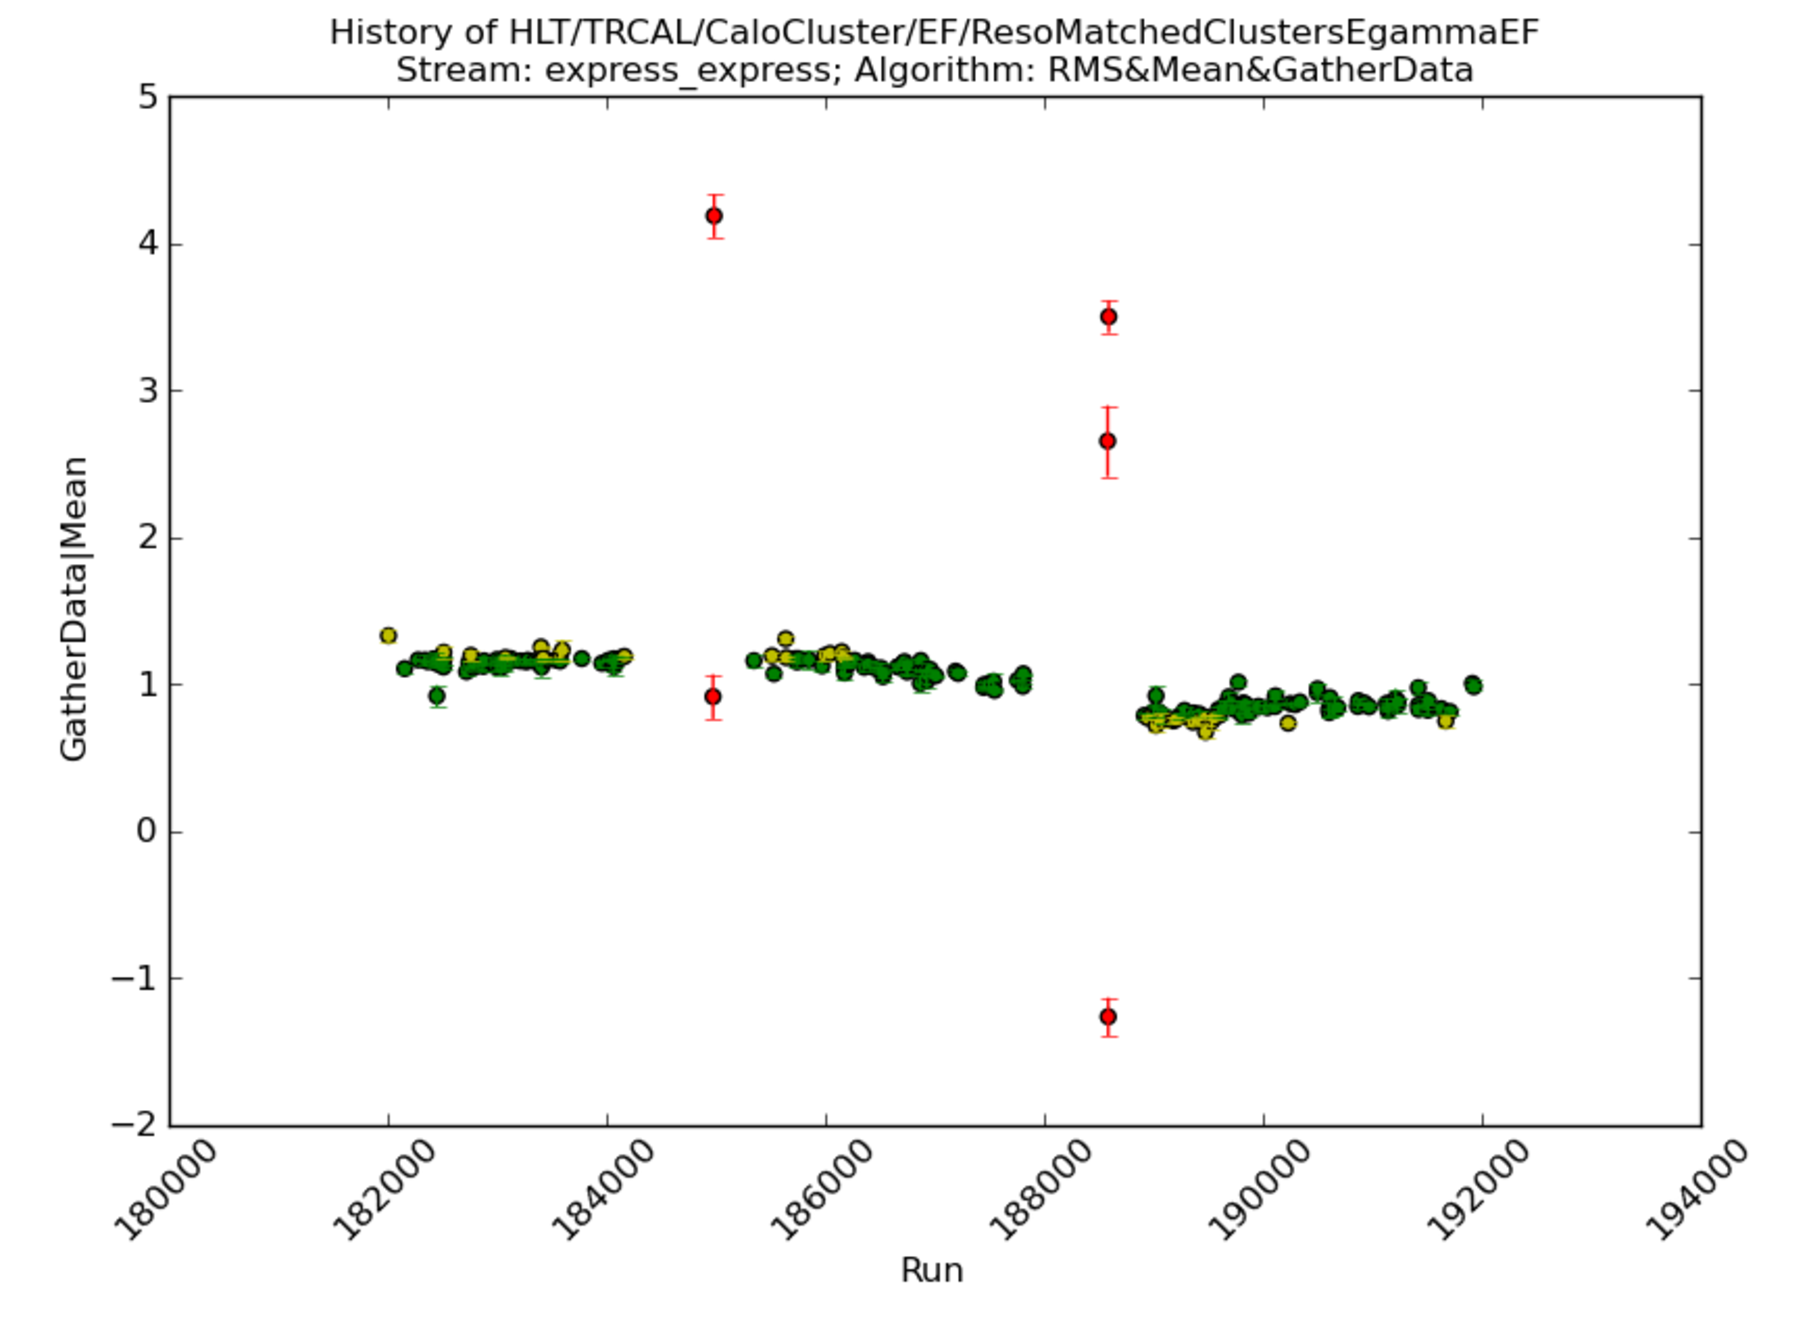
\includegraphics[width=1.0\textwidth]{figures/ServiceWork/EF_Reso_Range.pdf}
\caption[Mean EF EM cluster \et{} resolution as a function of run number]{
Mean EF EM cluster $\sigma(\et{})$ as a function of run number. 
\label{SW_egamma_EF_Reso_Range}}
\end{figure}


 
\subsection{Jets}
\label{HLTCalo:Jets}

%-Define the offline and two trigger jets 
%-need to explain what we really want to show.
%-Show the matching cuts
%-Explain the reason for the plots
%-For the plot, make sure we explain the red points.

Studying triggered and offline EM clusters monitors the EM calorimeter. 
Jets are used to study the hadronic calorimeter.
These jets consist of grouping of EM and hadronic clusters.

The \antikt{} jet-finding algorithm, which is described in Section \ref{sec:Theory:Jets}, was used with an R parameter of 0.4 for the offline jets.
The minimum \pt{} cut applied on the offline jets corresponds to the standard analysis cut of 20 GeV.


The L2 jet-finding is done using a cone algorithm.
The cone algorithm is seeded using a L1 RoI, and all deposits within the radius of the cone are combined, and a new cone centre is defined using the energy weighted position of the constituents.
With the new cone defined, any new deposits within the radius are again combined, and a new cone centre is defined.
This continues until the cone centre does not change.

The \antikt{} jet-finding algorithm is used for the EF jets. 
While it is the same jet-finding algorithm, the EF jets run over clusters that are close to the RoI.

In the 2012 data taking, calibration is applied to the EF jets to account for the non-compensating calorimeters. 

\subsubsection{Jet matching}

The trigger jets are matched to offline jets to allow them to be compared.
This matching is achieved by applying a \dr{} cut.
Figure \ref{SW_jet_L2_dR} shows the \dr{} between the offline jets and all L2 jets in the event.
As observed in the EM clusters, in (a) there are two peaks; one at $\dr{}\approx0$ and one at $\dr{}\approx3$.
The differences from the EM clusters are best seen in (b), the first peak is not quite at zero.
This is due to the $\phi$ resolution of the jets moving the \dphi{} away from zero. 
Figure \ref{SW_jet_EF_dR} shows the \dr{} between the offline jets and all EF jets in the event.
The distributions are similar to the L2 jet \dr{} distributions, with a peak just above zero, and one at $\dr{}\approx3$. 

A \dr{} matching cut of 0.4 is used for both the L2 and EF jets.
This value corresponds to the R value used in the jet-finding for both the trigger and offline jets.

\begin{figure}
\centering
\mbox{
              \subfigure[]{\epsfig{figure=figures/ServiceWork/Jets/L2_DRUnmatchedJetsJet.eps,width=0.5\textwidth}}\quad
              \subfigure[]{\epsfig{figure=figures/ServiceWork/Jets/L2_DRUnmatchedJetsZoomedJet.eps,width=0.5\textwidth}}\quad
                              }
\caption[\dr{} between offline and L2 jets]{\dr{} between the offline jet and all L2 jets in the event, shown with range (a) $0 - 6$ and (b) $0 - 1$ \label{SW_jet_L2_dR}}
\end{figure}

\begin{figure}
\centering
\mbox{
              \subfigure[]{\epsfig{figure=figures/ServiceWork/Jets/EF_DRUnmatchedJetsJet.eps,width=0.5\textwidth}}\quad
              \subfigure[]{\epsfig{figure=figures/ServiceWork/Jets/EF_DRUnmatchedJetsZoomedJet.eps,width=0.5\textwidth}}\quad
                              }
\caption[\dr{} between offline and EF jets]{\dr{} between the offline jet and all EF jets in the event, shown with range (a) $0 - 6$ and (b) $0 - 1$ \label{SW_jet_EF_dR}}
\end{figure}



\subsubsection{Monitored Distributions}

The jet monitoring uses the same distributions as the monitoring of the EM clusters.
The monitoring distributions shown in Figures \ref{SW_jet_L2EF_EtEt} - \ref{SW_jet_L2EF_Reco} are from run 203335, which was taken in 2012.

Figure \ref{SW_jet_L2EF_EtEt} shows the \et{} of the offline jet versus (a) the L2 and (b) the EF jets.
The \et{} comparison is used to check the linearity of the trigger jet \et{} to that of the offline jet.
The L2 trigger \et{} shows linearity to the offline jet \et{}, with the trigger jets \et{} being $\approx 60 \%$ of the offline jet \et{}. 
This is due to the different energy scales of the jets; whilst the offline are fully calibrated, the L2 trigger jets are at EM scale.
The \et{} of the EF jets agree well with the offline jets. 
This improvement is expected due to the calibration done on the EF jets.
Both the EF jets and the L2 jets have good linearity to the offline jet \et{}.

Figure \ref{SW_jet_L2EF_EtFrac_Eta} shows the \et{} fraction as a function of jet $\eta$ for (a) the L2 jets and (b) the EF jets.
The L2 jets have a mean \et{} fraction of $\approx 0.7$, whilst the EF jets have a mean \et{} fraction closer to one.  
This is again explained due to the jet energy scale of the trigger jets.
In both distributions, underlying differences between the trigger jets and offline jets can be seen in different regions of the detector.
The jumps in $f(\et{})$ at $|\eta|\sim1.2$ are due to the transition between the barrel and the tile calorimeters, and large fluctuations in jet \pt{} are anticipated.


Figure \ref{SW_jet_L2EF_Reco} shows the \et{} resolution of (a) the L2 jets and (b) the EF jets. 
As seen in previous figures, the L2 jets are $\approx 70 \%$ of the offline jets, due to the difference in calibration.
The mean of the \et{} resolution of the EF jets is close to zero. 
Problems in the detector, should show up in the plot, as a change in the mean.



\begin{figure}
\centering
\mbox{
              \subfigure[]{\epsfig{figure=figures/ServiceWork/Jets/L2_EtEtMatchedJet.eps,width=0.5\textwidth}}\quad
              \subfigure[]{\epsfig{figure=figures/ServiceWork/Jets/EF_EtEtMatchedJet.eps,width=0.5\textwidth}}\quad
                              }
\caption[Offline jet \et{} versus L2/EF jet \et{}]{
\et{} of the offline jet versus the \et{} of the matched (a) L2 and (b) EF jet.
\label{SW_jet_L2EF_EtEt}}
\end{figure}


\begin{figure}
\centering
\mbox{
              \subfigure[]{\epsfig{figure=figures/ServiceWork/Jets/L2_EtFracEtaMatchedJet.eps,width=0.5\textwidth}}\quad
              \subfigure[]{\epsfig{figure=figures/ServiceWork/Jets/EF_EtFracEtaMatchedJet.eps,width=0.5\textwidth}}\quad
                              }
\caption[\et{} fraction of L2 and EF jet to offline jet ]{
\et{} fraction of the (a) L2 and (b) EF jets to the offline jet \et{} as a function of $\eta$. 
\label{SW_jet_L2EF_EtFrac_Eta}}

\end{figure}

\begin{figure}
\centering
\mbox{
              \subfigure[]{\epsfig{figure=figures/ServiceWork/Jets/L2_ResoMatchedJetsJet.eps,width=0.5\textwidth}}\quad
              \subfigure[]{\epsfig{figure=figures/ServiceWork/Jets/EF_ResoMatchedJetsJet.eps,width=0.5\textwidth}}\quad
                              }
\caption[\et{} resolution between offline jet \et{} and L2/EF jet \et{}]{
\et{} resolution of (a) the L2 jets and (b) the EF jets. 
\label{SW_jet_L2EF_Reco}}
\end{figure}




\subsection{Summary}

Updates to the HLT cell monitoring and the addition of offline monitoring of the HLTCalo using physics objects such as jets are presented.
Cells have been masked to reduce the effect from noisy cells, and the EM and jet triggers have been monitored and observed to have good stability. 
Data where this has not been the case have not been used for physics analyses.


\chapter{In-Situ Validation of ATLAS Jet Reconstruction and Calibration}
\label{chp:JetPerf}
The response of the calorimter to jets can be defined using fully simulated MC samples as
\begin{equation}
\mathcal{R(\eta)} = \frac{\pt{}^{reco}(\eta)}{\pt{}^{truth}(\eta)}
\label{JetPerf:MCJetResp}
\end{equation}
where \pt{}$^{reco}$ is the \pt{} of the MC jet after full simulation of the detector, and  \pt{}$^{truth}$ is the \pt{} of the MC jet, before detector simulation. 
The truth and reco jets are matched using a \dr{} cut of 0.3.
%The calibration is done using the H1 method, which is described in \cite{ref:H1}. 

Jet response within the calorimeter varies as a function of $\eta$ due to the different calorimeter technology used and the varying levels of dead material, as shown in Figure \ref{JetPerf:MCResp}.
The default calibration procedure in ATLAS is to correct the energy and momentum by $\frac{1}{\mathcal{R(\eta)}}$.

\begin{figure}
\centering
\mbox{
              {\epsfig{figure=figures/JetPerformance/MCResponse-ref_ATLAS-CONF-2010-055.eps,width=\textwidth}}
                              }
\caption[]{ PYTHIA simulated jet EM-scale response as a function of reconstructed jet $\eta$ for different jet energies \cite{ref:EtaInter2010}
\label{JetPerf:MCResp}}
\end{figure}

The accuracy of the calibration depends how well the MC models the physics, such as ..., and how accurately if describes the detector geometry. 
In-situ methods are used to check the calibration and to assign a corresponding uncertainty.


********Add a section on the JES uncertainty contributions and link to paper ******
In the central region (\etaRange{0}{0.8}), the response and uncertainty from single particles in the calorimeter is used to give the JES uncertainty.  
This is done by  studying the charged particle response of the detector, gained from comparing charged tracks to isolated energy deposits.
********


Outside of this central region different in-situ methods are used to get contributions to the JES uncertainty.
One of the in-situ methods used to assess the uncertainty in the end cap (\etaRange{0.8}{2.8}) and forward (\etaRange{2.8}{4.5}) regions is pseudorapidity inter-calibration using dijets.
The jets in the central region, which are well understood, are used as a baseline to get relative calibration uncertainties in the end cap and forward regions. 

This method of extending the uncertainty outside the central region is achieved by using the \pt{} balance of dijet events to get a relative jet response between the 2 jets.
In a dijet topology, it is expected, that both jets should have the same transvere momentum, assuming that the jets arise from a $2\rightarrow2$ partonic scatter.
Using this assumption, the \pt{} imbalance can be expressed using the asymmetry, $\mathcal{A}$, defined as
\begin{equation}
\mathcal{A} =\frac{\pt{}^1 - \pt{}^2}{\ptave{}},
\label{JetPerf:Assym}
\end{equation}
where $\pt{}^1$ and $\pt{}^2$ are the transverse momentum of the two leading jets, and $\ptave{}$ is the average \pt{} of the two jets.
For imperfectly measured jets, the asymmetry would not be unity and a relative calorimeter response to a jet can be constructed using the asymmetry as,
\begin{equation}
 \frac{\pt{}^1}{\pt{}^2}=\frac{2+\mean{\mathcal{A}}}{2-\mean{\mathcal{A}}}.
\label{JetPerf:JetResp}
\end{equation}


For the balancing to work it is important that there is no other hard QCD emission in the interaction, this is achieved with a cut on the 3rd jet $\pt{}^3<0.25*\ptave{}$ and requiring the jets to be back-to-back in azimuth with a cut $\dphi{}>2.6$.

 

\section{In-Situ Validation of Jet Calibration}
\subsubsection{Standard Method for Dijet Balance}

In the standard method, one of the jets is required to be in a reference region where the jet is well calibrated and understood.
This jet is defined as the ``reference'' jet.
The other jet is the ``probe'' jet, and is used to probe the regions outside the reference region.


Given these definitions, Equations \ref{JetPerf:Assym} and \ref{JetPerf:JetResp} become,
\begin{equation}
\mathcal{A} =\frac{\pt{}^{probe} - \pt{}^{ref}}{\ptave{}}
\qquad
\rm{ and } 
\qquad
\frac{\pt{}^{ref}}{\pt{}^{probe}}=\frac{2+\mathcal{A}}{2-\mathcal{A}}=\frac{1}{\rm c},
\label{JetPerf:SM_Eqn}
\end{equation}
where $\rm c$ is the response ratio of the probe jet to the reference jet.  

Using this standard method, a asymmetry distribution, $\mathcal{A}_{ik}$ , is attained in bins of $\eta$ and $\phi$.
The ratio of responses, or inter-calibration factor, for the i-th $\eta$ and k-th $\ptave{}$ bin is defined as
\begin{equation}
\rm{c_{ik}} =\frac{2-\mean{\mathcal{A}_{ik}}}{2+\mean{\mathcal{A}_{ik}}},
\label{JetPerf:SM_CorrectionFactor}
\end{equation}
where \mean{\mathcal{A}_{ik}} is the mean value of the asymmetry distribution in the bin.


\subsubsection{Matrix Method for Dijet Balance}

The matrix method differs from the standard method by not requiring a specific reference region.
Instead of a probe and reference jet, there is a ``left'' jet and a ``right'' jet, where $\eta^{\mathrm{left}}<\eta^{\mathrm{right}}$.
As a result Equations \ref{JetPerf:Assym} and \ref{JetPerf:JetResp} become,
\begin{equation}
\mathcal{A} =\frac{\pt{}^{\mathrm{left}} - \pt{}^{\mathrm{right}}}{\ptave{}}
\label{JetPerf:MM_Assym}
\end{equation}
and 
\begin{equation}
\frac{\pt{}^{\mathrm{left}}}{\pt{}^{\mathrm{right}}}=\frac{2+\mathcal{A}}{2-\mathcal{A}}
\label{JetPerf:MM_CorrectionFactor}
\end{equation}

For given values of $\eta^{\mathrm{left}}$ and $\eta^{\mathrm{right}}$, the relative response between the two regions can be defined as 

\begin{equation}
\mathcal{R}_{ijk}= \frac{2-\mean{\mathcal{A}_{ ijk}}}{2+\mean{\mathcal{A}_{ ijk}}} = \frac{ c_{ik}^{\mathrm{left}}}{ c_{jk}^{\mathrm{right}}}
\label{JetPerf:MM_Response_Measured}
\end{equation}
where $i$, $j$ and $k$ are label bins in  $\eta^{\mathrm{left}}$, $\eta^{\mathrm{right}}$ and $\ptave{}$ respectively, and $\mean{\mathcal{A}}$ is the mean\footnote{The asymmetry distribution is fitted with a Gaussian function between -0.7 and 0.7, and the value of the fit is taken as the mean, unless there are low statistics, then the average of the asymmetry is taken} of the asymmetry distribution. 


For every $k$-th $\ptave{}$ bin, there exists $\sum\limits^N_{n=1}n$ relative responses, $\mathcal{R}_{ ijk}$, corresponding to different $\eta^{\mathrm{left}}$ and $\eta^{\mathrm{right}}$ bins ($i$,$j$).
A minimisation is performed to take into account the response measurements between many regions, to extract the inter-calibration factors for a specific $\eta$ region.
The inverse of the variance on each measured relative response, $\Delta\mathcal{R}_{ijk}$, is used to weight the equations in a minimisation equation,
\begin{equation}
\mathcal{M}_{k} = \sum\limits^N_{j=1} \sum\limits^N_{i=j}\left\{\frac{1}{\Delta\mathcal{R}_{ ijk}}( c_{jk}\mathcal{R}_{ ijk}- c_{ik} )\right\}^2 + X(c_{ik}).
\label{JetPerf:MM_Final}
\end{equation}

The first term in Equation \ref{JetPerf:MM_Final} is minimised to find the values of $c_{ik}$ that best agree with the measured $\mathcal{R}_{ijk}$. 
A trivial undesired solution is $c_{ik}=0$. 
The second term in \ref{JetPerf:MM_Final} is added to prevent this solution.
The specific form is 
\begin{equation}
X(c_{ik})= K(N^{-1}_{bins} \sum\limits^{N_{bins}}_{i=1} c_{ik} - 1 )^2,
\end{equation}
where K is a constant.
This term is a minimum when the average correction factor is equal to unity.
K is set to $10^6$, and its purpose is to penalise deviations of the average away from 1. 
For large values of K, the correction factors found are stable.
Once the minimised $c_{ik}$ values are found, these values are rescaled such that the correction factors at $|\eta|<1$ are equal to unity. 

The advantage of this method with respect to the standard method is that each relative response is calculated using every $\eta$ bin combination, which gives an increase in the statistics used, especially at larger $\eta$, when compared to the standard method which needed one of the jets to be in the central probe region.

\subsubsection{Two and Three Bin Example of Matrix Method}
To understand the matrix method, a two-bin and a three-bin case are discussed further.
The equation relating the two $\eta$ bins for the $k$-th \ptave{} bin is,  
\begin{equation}
\mathcal{M}_{k} = c_{2k}\mathcal{R_{\rm 12k}}- c_{1k}.
\label{JetPerf:Matrix_2binEquations}
\end{equation}
The equation is minimised when $c_{2k}\mean{\mathcal{R_{\rm 12k}}}= c_{1k}$ with a requirement that the average value is equal to unity.
Setting the first $\eta$ bin to the reference region with a $c_{2k}=1$, then 
\begin{equation}
c_{1k}=\mathcal{R_{\rm 12k}}= \frac{2-\mean{\mathcal{A_{\rm ijk}}}}{2+\mean{\mathcal{A_{\rm ijk}}}} 
\label{JetPerf:Matrix_2binEquations}
\end{equation}
which is the same as Equation \ref{JetPerf:SM_CorrectionFactor} used in the standard method.
For a three-bin case, with $\eta$ bin indices ${1,2,3}$ the equations are;
\begin{equation}
\begin{split}
c_{2k}\mathcal{R_{\rm 12k}}- c_{1k}; \\
c_{3k}\mathcal{R_{\rm 13k}}- c_{1k}; \\
c_{3k}\mathcal{R_{\rm 23k}}- c_{2k}.
\end{split}
\label{JetPerf:Matrix_3binEquations}
\end{equation}
For the three-bin example the minimisation equation is,
\begin{equation}
\mathcal{M}_{k} =\left(\frac{c_{2k}\mathcal{R_{\rm 12k}}- c_{1k}}{\Delta\mathcal{R_{\rm 12k}}}\right)^2+
\left(\frac{c_{3k}\mathcal{R_{\rm 13k}}- c_{1k}}{\Delta\mathcal{R_{\rm 13k}}}\right)^2+
\left(\frac{c_{3k}\mathcal{R_{\rm 23k}}- c_{2k}}{\Delta\mathcal{R_{\rm 23k}}}\right)^2+ X(c_{ik}).
\label{JetPerf:Matrix_3binEquations2}
\end{equation}
The minimisation attempts to minimise the first three terms, while also keeping the mean correction at unity (fourth term).
The variance on $\mathcal{R}$, $\Delta\mathcal{R}$, is smaller for high statistics measurements of $\mathcal{R}$.
Including the variance in the minimisation, gives measurements with a low variance a higher importance in determining the values of $c_{ik}$. 


\section{2011 Study of Pile-up Dependance}
\subsubsection{Event Selection}

The jets in the analysis are reconstructed using the \antikt{} algorithm with a distance parameter $R=0.4$ and calibrated using the JES scheme (discussed in Section \ref{sec:Det:Jets}).
The analysis requires that a single jet trigger has passed.
Triggers are used if they are in the plateau region of the turn-on curve, corresponding to a greater than $99\%$ efficiency.
The trigger used for a given \ptave{} is shown in Table \ref{JetPerf:Triggers}.
A trigger with name jX requires an EF-level trigger jet with EM scale $\pt{}>$X GeV.
\begin{table}
%\footnotesize
\centering
\begin{tabular}{  c | c }
\hline
\hline
\ptave{} & Trigger\\
$[\rm GeV]$ & \\
\hline
$22-30$   & j10 \\
$30-40$   & j15 \\
$40-55$   & j20 \\
$55-75$   & j30 \\
$75-100$  & j40 \\
$100-130$ & j55 \\
$130-170$ & j75 \\
$170-220$ & j100 \\
$220-300$ & j135 \\
$300-400$ & j180 \\
\hline
\hline
\end{tabular}
\caption[Trigger strategy for dijet \pt{} balance in 2011]{
Trigger strategy for the different dijet \ptave{}. 
\label{JetPerf:Triggers}}
\end{table}
The data are required to be in luminosity blocks when all ATLAS sub-detectors are fully functioning. 

To ensure the $2\rightarrow2$ scattering topology the \dphi{} between the two jets is required to be greater than $2.5$ rad and events containing a third jet with $\pt{} >0.25~ \ptave{}$ are removed.
The reference region that is used to do the final rescaling of the responses in the matrix method is \etarange{-0.8}{0.8}.

\subsubsection{Basic Asymmetry and Response Distributions}

Figures \ref{JetPerf:Asym_j15} and \ref{JetPerf:Asym_j30} each show two asymmetry distributions for jets falling in (a) two central regions, $-0.8<\eta_{left}<-0.1$ and $0.1<\eta_{right}<0.8$, and (b) one central region and one more forward region, $0.1<\eta_{left}<0.8$ and $2.1<\eta_{right}<2.8$. 
Each asymmetry distributions have been fitted with a Gaussian function from $-0.7<\mathcal{A}<0.7$.

Figure \ref{JetPerf:Asym_j15} shows asymmetry distributions for $30<\ptave{}<40$ GeV jets.
The peak of the fitted asymmetry for both jets falling in the central region is $0.006$, which corresponds to a very small \pt{} imbalance of $\mean{\pt{}^{right}}= 0.994 \mean{\pt{}^{left}}$.
The peak of the fitted asymmetry for one jet falling in the central region and the other in a forward region is $0.023$, which corresponds to a \pt{} imbalance of $\mean{\pt{}^{right}}= 0.98 \mean{\pt{}^{left}}$.

Figure \ref{JetPerf:Asym_j30} shows asymmetry distributions for $55<\ptave{}<75$ GeV jets.
The peak of the fitted asymmetry for both jets falling in the central region is $0.003$, which corresponds to very small \pt{} imbalance of $\mean{\pt{}^{right}}= 0.997 \mean{\pt{}^{left}}$. 
The peak of the fitted asymmetry for one jet falling in the central region and the other in a forward region is $0.007$, which corresponds to a \pt{} imbalance of $\mean{\pt{}^{right}}= 0.993 \mean{\pt{}^{left}}$.

The width in the asymmetry distributions arises due to the jet energy resolution of the two jets and the peak value of the fitted asymmetry relates to the relative responses of the two regions.
In the distributions for both the low and high \ptave{} jets, the case where both jets fall into central regions has a lower \pt{} imbalance than the case where one jet falls into a forward region.  
When both jets fall into the barrel region they are better calibrated, as the barrel region is well understood (through test beam information and single hadron response) and has little dead material.
However, when one jet is further forward, is falls into the end-cap region of the calorimeter and the difference observed could be due to the differing abilities to calibrate the different parts of the detector. 
The spread of asymmetry is smaller for higher \ptave{} jets, which is due to the improved resolution for higher \pt{} jets.


Figures \ref{JetPerf:ResponseMatrix_30_40_j15} and \ref{JetPerf:ResponseMatrix_55_75_j30} show the the response matrices, which are used by the minimisation, for jets in the range $30<\ptave{}<40$~GeV and $55<\ptave{}<75$ GeV, respectively.
The low \ptave{} jets have a larger range of relative responses than the high \ptave{} jets, with some bins deviating from unity by up to $6\%$.
In both response matrices the higher $\eta$ bins have a larger spread of responses than the more central bins.


Figure \ref{JetPerf:PtComp} shows the relative response as a function of detector $\eta$ for $22<\ptave{}<30$ GeV jets, $30<\ptave{}<40$ GeV jets, and $55<\ptave{}<75$ GeV jets. 
The largest relative response occurs for low \ptave{}.
There is a relative response of about $1.02$ at $|\eta|=1$ which corresponds to the crack region between the tile barrel and tile extended barrel. 
This crack can be seen in the jet energy EM-scale response in Figure \ref{Det:MCResp}.
For low \pt{} jets, the calibration has over-calibrated the jets in this crack region. 
For the medium and high jet \pt{} ranges shown, the relative response for $|\eta|<1$ is very close to unity.
The response at higher $\eta{}$ deviates away from unity, and as the jet \pt{} increases this deviation reduces. 

\begin{figure}
\centering
\mbox{
              \subfigure[]{\epsfig{figure=figures/JetPerformance/2011/j15zvar4_6.eps,width=0.8\textwidth}}
}
\mbox{
              \subfigure[]{\epsfig{figure=figures/JetPerformance/2011/j15zvar6_9.eps,width=0.8\textwidth}}
}
\caption[Example asymmetry distribution for jets with $30<\ptave{}<40$ GeV]{
Asymmetry distribution for jets with $30<\ptave{}<40$ GeV with (a) $-0.8<\eta_{left}<-0.1$ and $0.1<\eta_{right}<0.8$ and (b)  $0.1<\eta_{left}<0.8$ and $2.1<\eta_{right}<2.8$.
The distribution is fitted using a Gaussian function between $\rm{-0.7<A<0.7}$ and the fit result and error is shown as is the mean and error on the mean. 
\label{JetPerf:Asym_j15}}
\end{figure}

\begin{figure}
\centering
\mbox{
              \subfigure[]{\epsfig{figure=figures/JetPerformance/2011/j30zvar4_6.eps,width=0.8\textwidth}}
}
\mbox{
              \subfigure[]{\epsfig{figure=figures/JetPerformance/2011/j30zvar6_9.eps,width=0.8\textwidth}}
}

\caption[Example asymmetry distribution for jets with $55<\ptave{}<75$ GeV]{
Asymmetry distribution for jets with $55<\ptave{}<75$ GeV with (a) $-0.8<\eta_{left}<-0.1$ and $0.1<\eta_{right}<0.8$ and (b)  $0.1<\eta_{left}<0.8$ and $2.1<\eta_{right}<2.8$.
The distribution is fitted using a Gaussian function between $\rm{-0.7<A<0.7}$ and the fit result and error is shown as is the mean and error on the mean. 
\label{JetPerf:Asym_j30}}
\end{figure}

\begin{figure}
\centering
\mbox{
              \epsfig{figure=figures/JetPerformance/2011/j15TwoDPlotBoth.eps,width=0.9\textwidth}
}
\caption[The response matrix for jets with $30<\ptave{}<40$ GeV]{
Response matrix for $30<\ptave{}<40$ GeV for jets which passed the j15 trigger. 
The text in the bins corresponds to the percentage difference between the response and unity.
\label{JetPerf:ResponseMatrix_30_40_j15}}
\end{figure}

\begin{figure}
\centering
\mbox{
              \epsfig{figure=figures/JetPerformance/2011/j30TwoDPlotBoth.eps,width=0.9\textwidth}
}
\caption[The response matrix for jets with $55<\ptave{}<75$ GeV]{
Response matrix for $55<\ptave{}<75$ GeV for jets which passed the j30 trigger. 
The text in the bins corresponds to the percentage difference between the response and unity.
\label{JetPerf:ResponseMatrix_55_75_j30}}
\end{figure}


\begin{figure}
\centering
\mbox{
              \epsfig{figure=figures/JetPerformance/2011/ResponseAvePtComp.eps,width=0.9\textwidth}
}
\caption[Relative response as a function of $\eta$]{
Relative response as a function of detector $\eta$ for jets with $22<\ptave{}<30$ GeV, $30<\ptave{}<40$ GeV and $55<\ptave{}<75$ GeV.
\label{JetPerf:PtComp}}
\end{figure}



\subsubsection{Effect of Pile-up on Dijet Balance}

The \pt{} balance of dijets events can be used to construct a correction factor or used to ascertain aspects of the JES uncertainty \cite{ref:JES}.
In this section it is used as a cross-check of JES uncertainty components from pile-up.
This is done by calculating the relative response for events with different levels of pile-up.

Two estimators of the amount of pile-up used are the number of primary vertices, $\mathrm{N_{PV}}$, and the mean number of interactions per bunch crossing, $\mu$.
Figure \ref{JetPerf:NPV_Mu} shows (a) the $\mathrm{N_{PV}}$ distribution and (b) the $\mu$ distributions.
$\mathrm{N_{PV}}$ and $\mu$ cuts are chosen to select events with different amount of pile-up.
For the $\mathrm{N_{PV}}$ cuts, three slices are chosen such that each has good statistics, but also has differences in the average $\mathrm{N_{PV}}$ per slice.
Three $\mathrm{N_{PV}}$ regions are defined to select different pile-up conditions, \Range{\mathrm{N_{PV}}}{0}{2}, \Range{\mathrm{N_{PV}}}{3}{6}, and  $\rm \mathrm{N_{PV}}\ge7$, with an average $\mathrm{N_{PV}}$ of 2.48, 4.48 and 7.71, respectively. 
For the $\mu$ cuts, two slices are chosen, one that includes the peak, and one that includes the tail, both of with have good statistics. 
Two $\mu$ regions are defined, \Range{\mu}{0}{7} and  $\mu > 7$, with an average $\mu$ of 5.33 and 9.94, respectively. 
Data points which have no cuts on $\mu$ or $\mathrm{N_{PV}}$ are also shown for comparative purposes.
These have an average $\mathrm{N_{PV}}$ and $\mu$ of 5.19 and 6.48, respectively.



%High NPV:  Ave NVP:  7.71314
%Med NPV:  Ave NVP:  4.48111
%Low NPV:  Ave NVP:  2.47613
%Standard: Average mu : 6.47532  Ave NVP:  5.18579


Figures \ref{JetPerf:PileupComp_j10}, \ref{JetPerf:PileupComp_j15} and \ref{JetPerf:PileupComp_j20}  show the relative response as a function of detector $\eta$ for jets with $22<\ptave{}<30$ GeV, $30<\ptave{}<40$ GeV and $55<\ptave{}<75$ GeV, respectively, for different $\mathrm{N_{PV}}$ ranges.
For the $22<\ptave{}<30$ GeV jets, the relative response in the forward bins is lower for jets in the low pile-up conditions than the jets using the full data.
The medium has a higher relative response in the bins outside the reference region.
The spread of the three different $\mathrm{N_{PV}}$ points is contained within $\approx 4\%$ and there is no systematic difference in spread as a function of $\eta{}$.
For the $30<\ptave{}<40$ GeV jets, the spread has decreased to within $\approx 2\%$. 
In the forward bins at negative $\eta$, the low pile-up and high pile-up have a higher and lower response than the average, respectively, however this is probably just fluctuations as there is no pathological effect.
For the  $55<\ptave{}<75$ GeV jets, the spread is within $\approx 1\%$, and there is no obvious trend in the differences between the different pile-up conditions.

The observation that the low \ptave{} jets are affected more, is not unexpected, as pile-up can be considered to add a fixed amount of additional energy per additional proton-proton interaction.
This additional energy will be a larger fraction of a low \pt{} jet than of a high \pt{} jet at the same rapidity, and so the net effect will be larger.
It might be expected that the jets in the lower pile-up conditions should have a lower relative response than jets in a higher pile-up condition, however the EM+JES calibration does an pile-up offset correction, which should account for this.


Figures \ref{JetPerf:MuComp_j10}, \ref{JetPerf:MuComp_j15} and \ref{JetPerf:MuComp_j20}  show the relative response as a function of detector $\eta$ for jets with $22<\ptave{}<30$ GeV, $30<\ptave{}<40$ GeV and $55<\ptave{}<75$ GeV respectively for different $\mu$ ranges.
For the $22<\ptave{}<30$ GeV jets, the spread  is $\approx 3\%$ for $-2.8\le\eta\le-2$ range, but for most bins it is within $ 1-2\%$.
In most of the bins the low pile-up sample has a responses slightly higher than the response from the high pile-up samples.
For the $30<\ptave{}<40$ GeV jets, the relative responses are closer to unity than for the lower \ptave{} jets.
The spread is consistent $2\%$ with approximately equal number of bins where the low pile-up sample is above the high pile-up sample, than the reverse.
For the $55<\ptave{}<75$ jets, the spread is $<1\%$ for all but one bin, and the relative response is close to one.  
As with the assessment of the pile-up using the $\mathrm{N_{PV}}$, the spread shows a general downwards trend for higher \ptave{}, though the jets with $30<\ptave{}<40$ GeV have a marginally higher spread than $22<\ptave{}<30$ GeV, but without the larger fluctuations,

The observed effects from $\mathrm{N_{PV}}$ and $\mu$ are $~3-4\%$ for low \ptave{} jets, and reduce to $~1\%$ for jets with $55<\ptave{}<75$.
These spreads of values for the relative response show agreement to the JES uncertainty due to pile-up using the method described in \cite{ref:Pileup} and combined to the JES uncertainty in \cite{ref:JES2011}.



\begin{figure}
\centering
\mbox{
              \subfigure[]{\epsfig{figure=figures/JetPerformance/2011/NPVDist.eps,width=0.5\textwidth}}
              \subfigure[]{\epsfig{figure=figures/JetPerformance/2011/MuDist.eps,width=0.5\textwidth}}
                              }
\caption[Number of primary vertices and $\mu{}$ for 2011 data]{
(a) The $\mathrm{N_{PV}}$ distribution and (b) the $\mu$ distribution for 2011 data.
\label{JetPerf:NPV_Mu}}
\end{figure}



\begin{figure}
\centering
\mbox{
              \epsfig{figure=figures/JetPerformance/2011/ResponseNPVj10Comp.eps,width=0.9\textwidth}
}
\caption[Relative response as a function of $\eta$ for 3 different pile-up conditions, based on $\mathrm{N_{PV}}$, for jets with $22<\ptave{}<30$ GeV]{
Relative response as a function of detector $\eta$ for jets with $22<\ptave{}<30$ GeV.
Relative responses are shown for events with \Range{\mathrm{N_{PV}}}{0}{2}, \Range{\mathrm{N_{PV}}}{3}{6}, $\rm \mathrm{N_{PV}}\ge7$ and all $\mathrm{N_{PV}}$. 
\label{JetPerf:PileupComp_j10}}
\end{figure}



\begin{figure}
\centering
\mbox{
              \epsfig{figure=figures/JetPerformance/2011/ResponseNPVj15Comp.eps,width=0.9\textwidth}
              %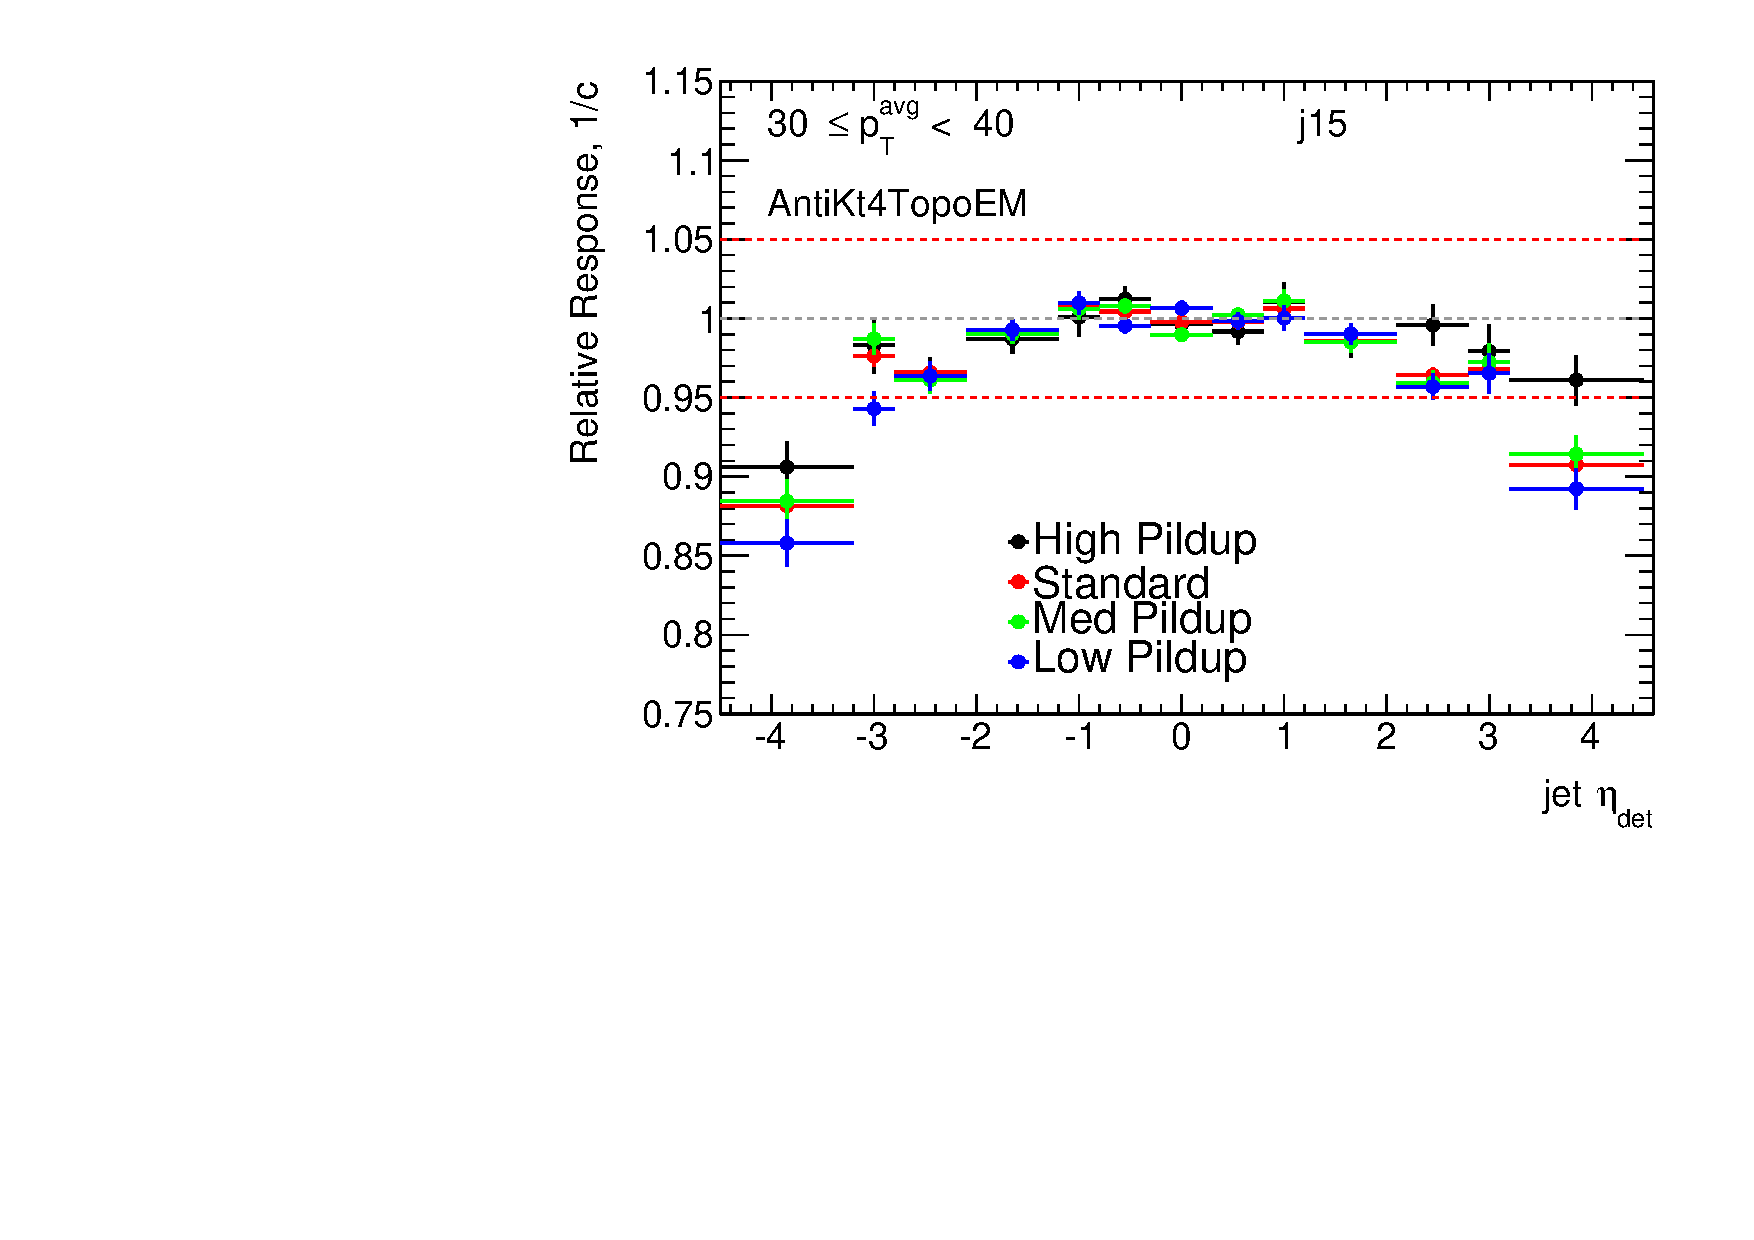
\includegraphics[width=0.8\textwidth]{figures/JetPerformance/2011/Pileup/PileupComp_AntiKt4TopoEM_j15_30-40Uncorrected.pdf}
}
\caption[Relative response as a function of $\eta$ for 3 different pile-up conditions, based on $\mathrm{N_{PV}}$, for jets with $30<\ptave{}<40$ GeV]{
Relative response as a function of detector $\eta$ for jets with $30<\ptave{}<40$ GeV.
Relative responses are shown for events with \Range{\mathrm{N_{PV}}}{0}{2}, \Range{\mathrm{N_{PV}}}{3}{6}, $\rm \mathrm{N_{PV}}\ge7$ and all $\mathrm{N_{PV}}$. 
\label{JetPerf:PileupComp_j15}}
\end{figure}

\begin{figure}
\centering
\mbox{
              \epsfig{figure=figures/JetPerformance/2011/ResponseNPVj30Comp.eps,width=0.9\textwidth}
              %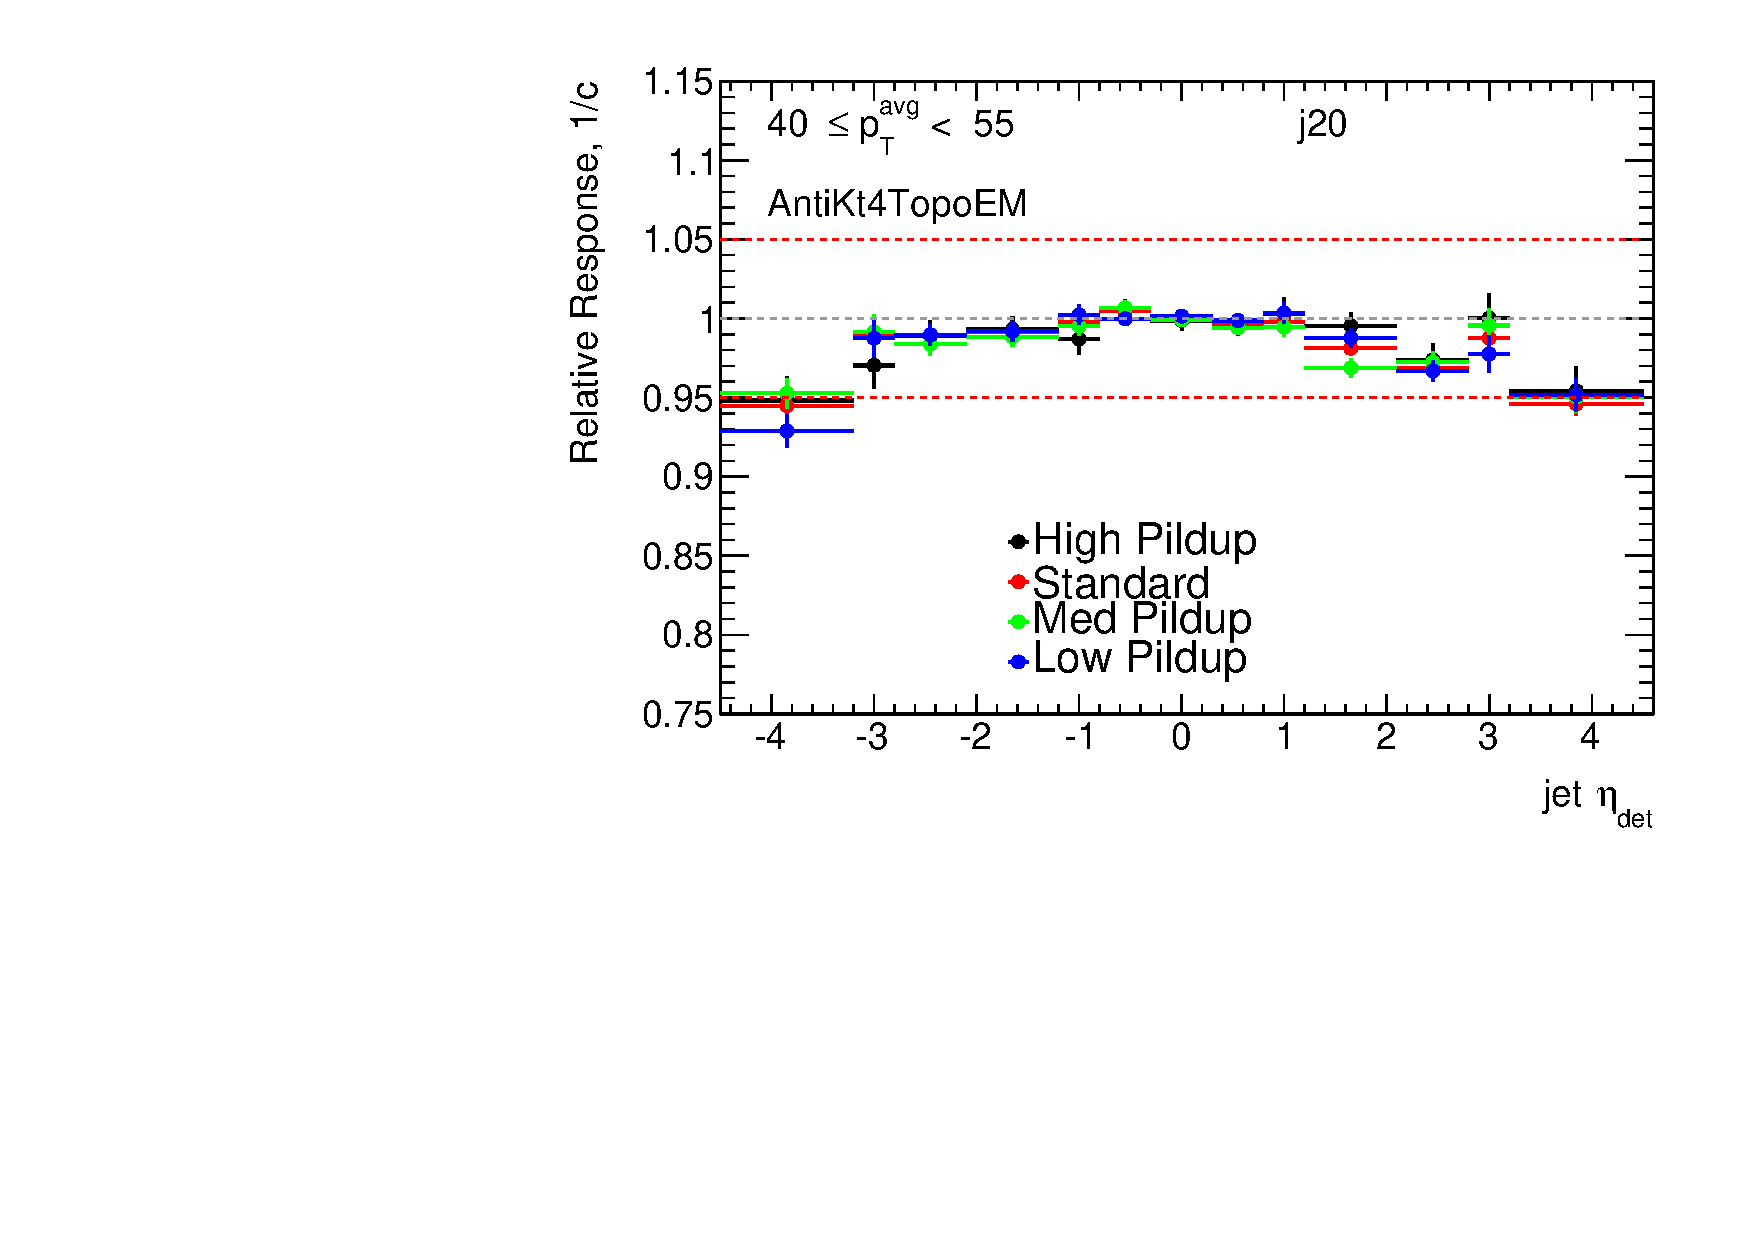
\includegraphics[width=0.8\textwidth]{figures/JetPerformance/2011/Pileup/PileupComp_AntiKt4TopoEM_j20_40-55Uncorrected.pdf}
}
\caption[Relative response as a function of $\eta$ for 3 different pile-up conditions, based on $\mathrm{N_{PV}}$, for jets with $55<\ptave{}<75$ GeV]{
Relative response as a function of detector $\eta$ for jets with $55<\ptave{}<75$ GeV.
Relative responses are shown for events with \Range{\mathrm{N_{PV}}}{0}{2}, \Range{\mathrm{N_{PV}}}{3}{6}, $\rm \mathrm{N_{PV}}\ge7$ and all $\mathrm{N_{PV}}$. 
\label{JetPerf:PileupComp_j20}}
\end{figure}

\begin{figure}
\centering
\mbox{
              \epsfig{figure=figures/JetPerformance/2011/Responsemuj10Comp.eps,width=0.9\textwidth}
              %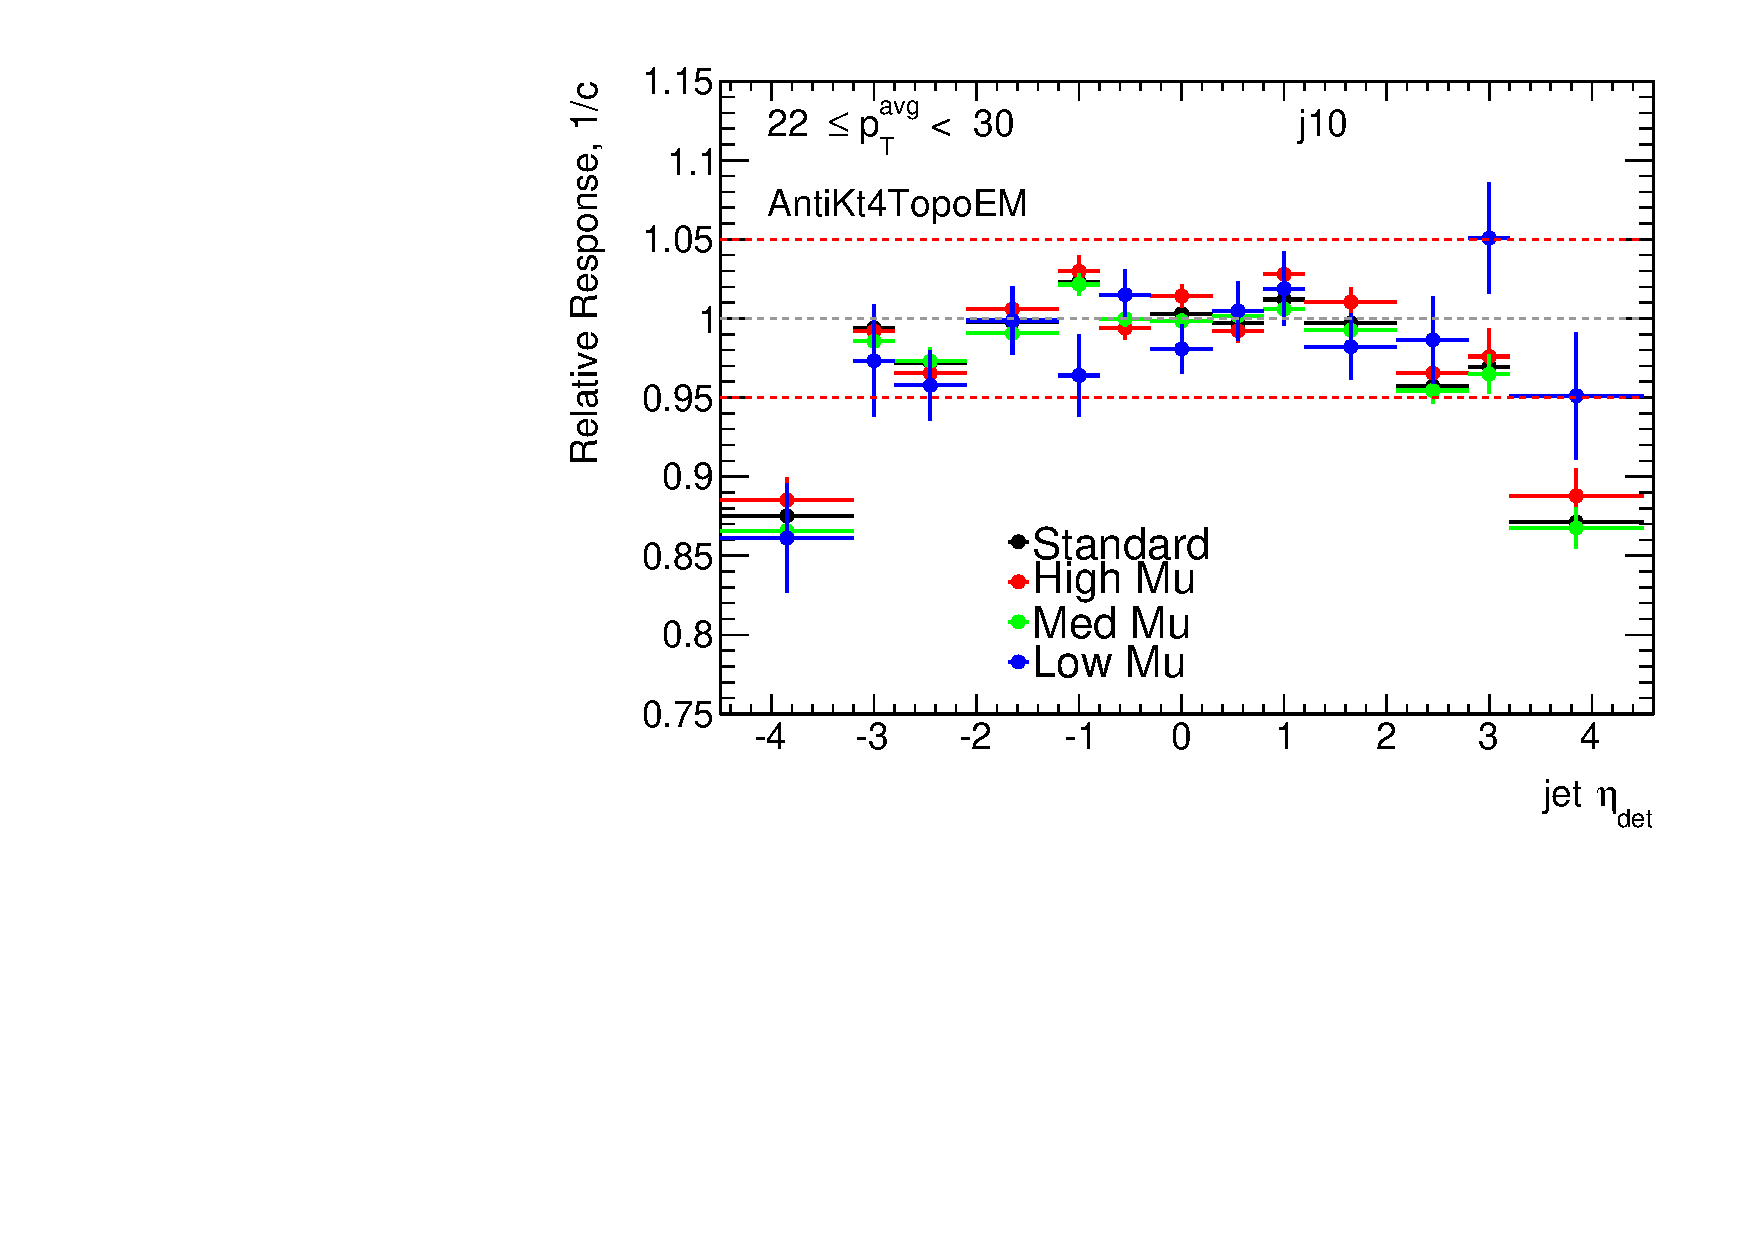
\includegraphics[width=0.8\textwidth]{figures/JetPerformance/2011/Pileup/MuComp_AntiKt4TopoEM_j10_22-30Uncorrected.pdf}
}
\caption[Relative response as a function of $\eta$ for 2 different pile-up conditions, based on $\mu{}$, for jets with $22<\ptave{}<30$ GeV]{
Relative response as a function of detector $\eta$ for jets with $22<\ptave{}<30$ GeV.
Relative responses are shown for events with \Range{\mu}{0}{6}, $\rm \mu\ge6$ and all $\mu$. 
\label{JetPerf:MuComp_j10}}
\end{figure}



\begin{figure}
\centering
\mbox{
              \epsfig{figure=figures/JetPerformance/2011/Responsemuj15Comp.eps,width=0.9\textwidth}
              %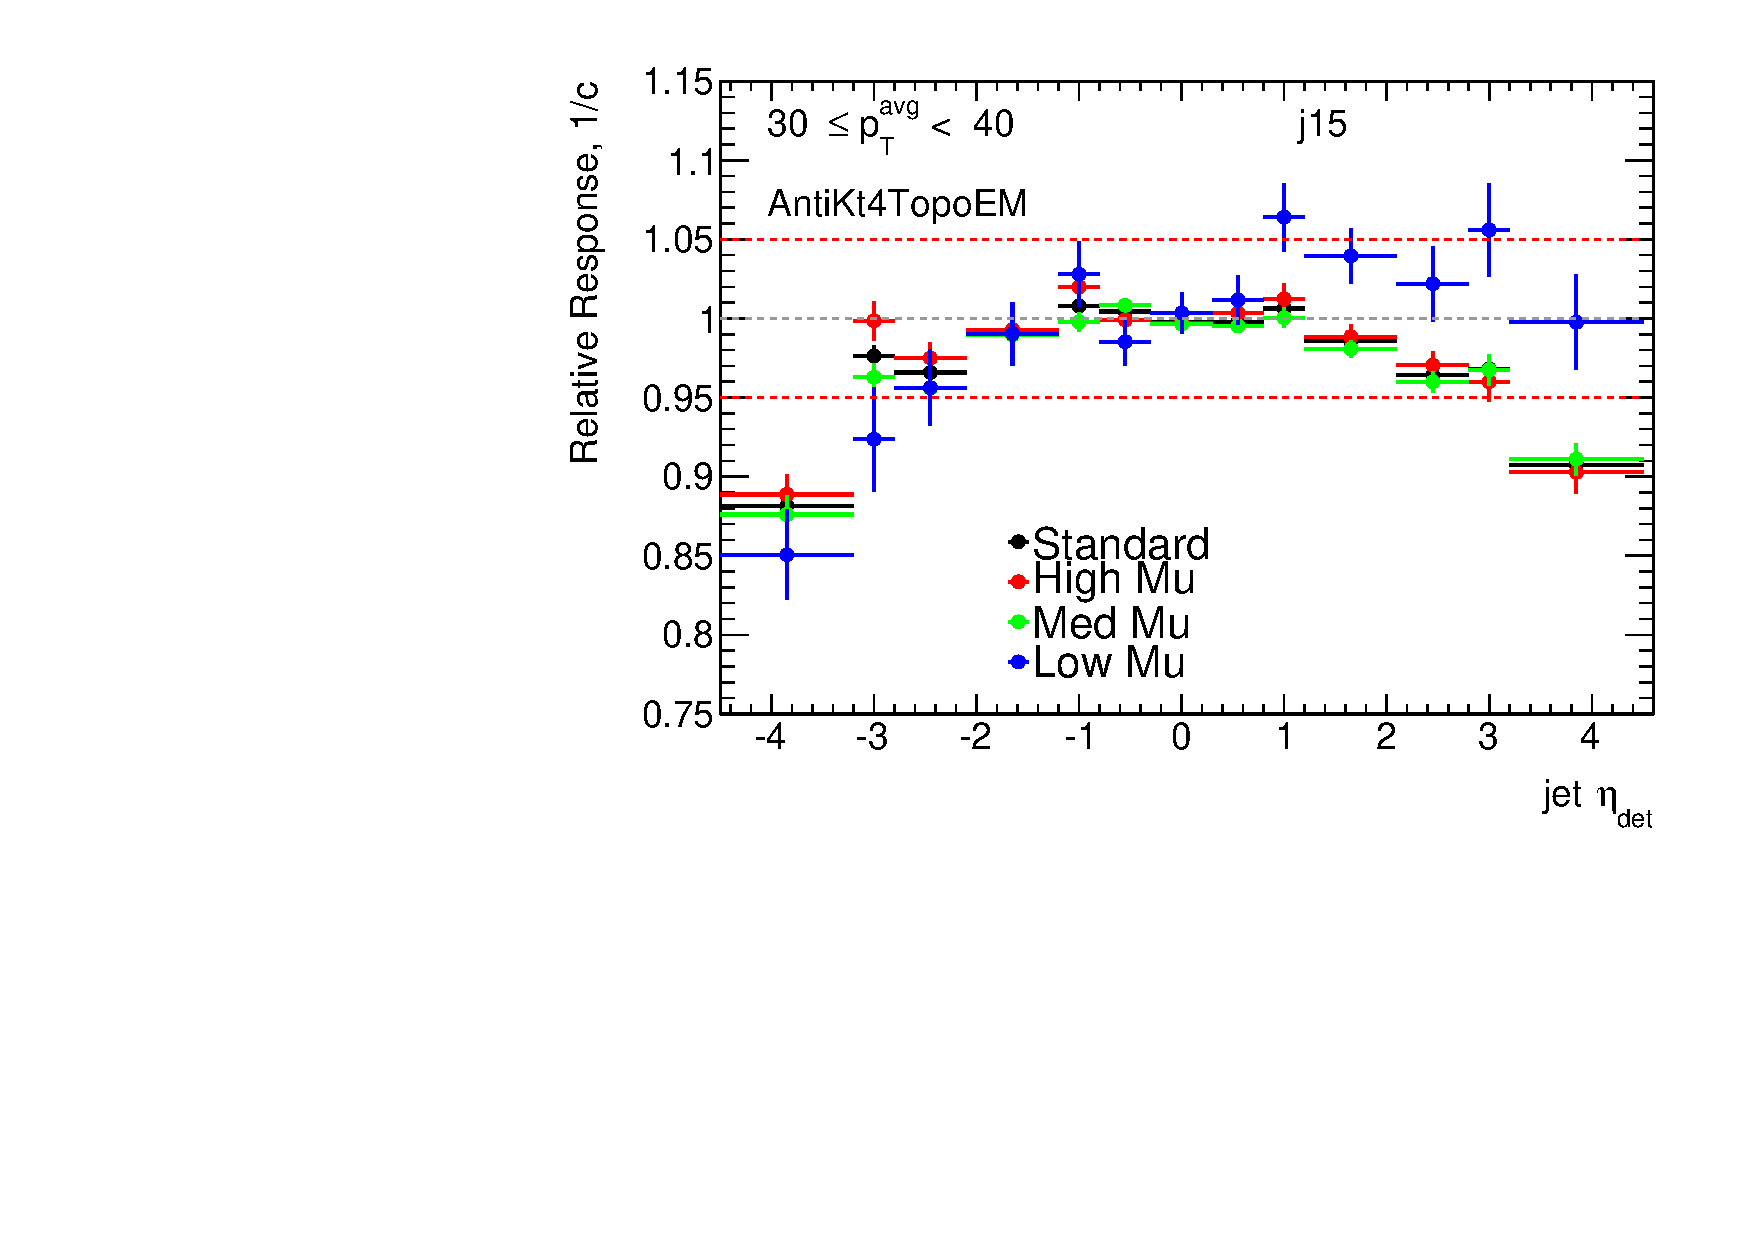
\includegraphics[width=0.8\textwidth]{figures/JetPerformance/2011/Pileup/MuComp_AntiKt4TopoEM_j15_30-40Uncorrected.pdf}
}
\caption[Relative response as a function of $\eta$ for 2 different pile-up conditions, based on $\mu{}$, for jets with $30<\ptave{}<40$ GeV]{
Relative response as a function of detector $\eta$ for jets with $30<\ptave{}<40$ GeV.
Relative responses are shown for events with \Range{\mu}{0}{6}, $\rm \mu\ge6$ and all $\mu$. 
\label{JetPerf:MuComp_j15}}
\end{figure}

\begin{figure}
\centering
\mbox{
              \epsfig{figure=figures/JetPerformance/2011/Responsemuj30Comp.eps,width=0.9\textwidth}
              %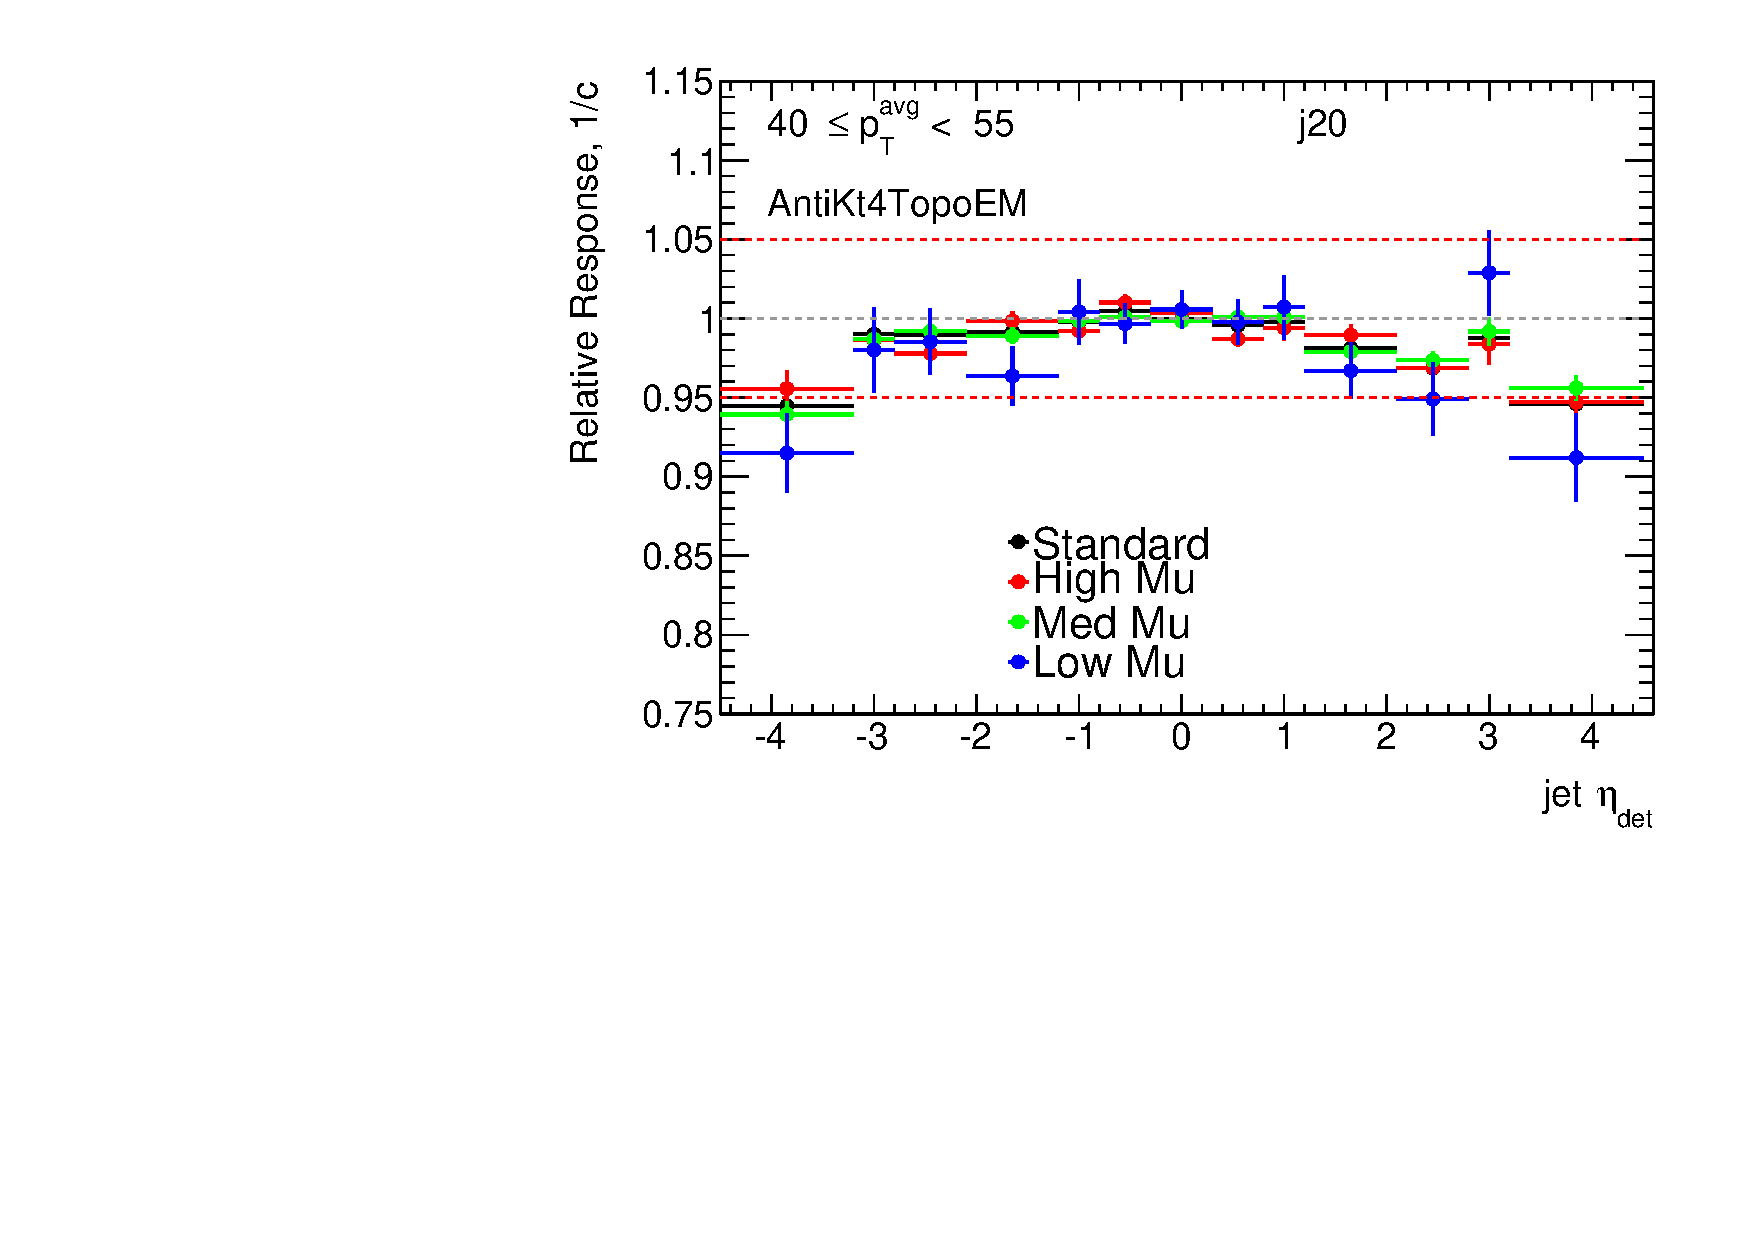
\includegraphics[width=0.8\textwidth]{figures/JetPerformance/2011/Pileup/MuComp_AntiKt4TopoEM_j20_40-55Uncorrected.pdf}
}
\caption[Relative response as a function of $\eta$ for 2 different pile-up conditions, based on $\mu{}$, for jets with $55<\ptave{}<75$ GeV]{
Relative response as a function of detector $\eta$ for jets with $55<\ptave{}<75$ GeV.
Relative responses are shown for events with \Range{\mu}{0}{6}, $\rm \mu\ge6$ and all $\mu$. 
\label{JetPerf:MuComp_j20}}
\end{figure}


\section{2010 Forward Jet Validation}
In 2010, the dijet \pt{} balance method was not used to recalibrate the jets, but was used to assess the uncertainty on the JES calibration factors.
However, the relative jet response \cite{ref:EtaInter2010} shows a difference in the forward region for MC and data.
The difference between the data and MC jet responses could either originate from physics or the detector effects described in Section \ref{sec:Det:Jets}. 
Until the source of the differences is determined, these relative response factors should not be used to calibrate the jets for physics analysis.
However, they are used to test the closure of the calibration and to see the difference between data and MC can be resolved.

Using the ratio of the relative response factors from the MC and the data, the residual correction, 

\begin{equation}
\mathcal{C_{\rm{in-situ}}} = \frac{\rm{c_{MC}}}{\rm{c_{Data}}}
\label{JetPerf:ResidualCorrection}
\end{equation}
is calculated, where ${1}/{\rm{c_{MC}}}$ and ${1}/{\rm{c_{Data}}}$ are the relative response factors for MC and data, respectively. 


Figure \ref{JetPerf:EtaData} shows the jet $\eta$ distribution for (a) \pt{} $>30$ GeV from the Min Bias trigger and (b) \pt{}$>50$ GeV from the calorimeter trigger stream. 
The in-situ calibrated data has a much better agreement with the MC than the uncorrected data in both plots. 
There are still differences in the forward region, but overall the differences are smaller than $10\%$.

Figure \ref{JetPerf:E_PtData} shows (a) the jet energy  and  (b) the \pt{} distributions  for jets in the region \etaRange{3.2}{4.5}  for \pt{}$>20$ GeV. 
The energy distribution shows improvements in agreement between the MC after the data has been calibrated.
The \pt{} distribution shows smaller differences for the in-situ calibrated data.

These results show that calibration brings the data into  closer agreement with the MC, giving confidence to the method and the results.
This confidence resulted in the decision to use the dijet \pt{} balance method to calibrate the jets in the 2011 sample. 
These plots were published in an ATLAS conference note \cite{ref:EtaInter2010}.


\begin{figure}
\centering
\mbox{
              \subfigure[]{\epsfig{figure=figures/JetPerformance/EtaDist30GeV.eps,width=0.5\textwidth}}\quad
              \subfigure[]{\epsfig{figure=figures/JetPerformance/EtaDist50GeV.eps,width=0.5\textwidth}}\quad
}
\caption[Effect of additional calibration on the jet $\eta$ distribution]{
$\eta$ distribution for jets with (a) \pt{} $>30$ GeV from the Min Bias trigger and (b) \pt{} $>50$ GeV from the calorimeter trigger stream. 
Uncorrected data (open black circles) and corrected data (red circles) are shown along with the reference MC. 
\label{JetPerf:EtaData}}
\end{figure}

\begin{figure}
\centering
\mbox{
              \subfigure[]{\epsfig{figure=figures/JetPerformance/EDist.eps,width=0.5\textwidth}}\quad
              \subfigure[]{\epsfig{figure=figures/JetPerformance/PtDist.eps,width=0.5\textwidth}}\quad
}
\caption[Effect of additional calibration on the jet energy and \pt{} distributions for jets in the FCal]{
(a) Jet energy and (b) jet \pt{} for the region \etaRange{3.2}{4.5}.
Uncorrected data (open black circles) and corrected data (red circles) are shown along with the reference MC. 
\label{JetPerf:E_PtData}}
\end{figure}


\section{ Forward Jet Properties}
The internal structure of jets in the forward region were examined using 2010 data to assess how well the MC simulation reproduces the data.
The transverse size of the jet is quantified using the jet width,
\begin{equation}
\mathrm{Width}=\frac{\sum (r^{\mathrm{cluster}} \times \et{}^{\mathrm{cluster}}) }{\sum \et{}^{\mathrm{cluster}}},
\label{JetPerf:Width}
\end{equation}
where the sums are over all clusters within the jet, and $r^{\mathrm{cluster}}$ is the distance of each cluster from the jet centre.
Another important jet observable is the electromagnetic fraction (EMF), which is the fraction of the total jet energy (at EM scale) coming from electromagnetic clusters.


Figure \ref{JetPerf:Width_EMF} (a) shows the jet width for jets in the forward region.
Figure \ref{JetPerf:Width_EMF} (b) shows the EMF for jets in the forward region.
The data are compared to PYTHIA using three different physics lists which use different calorimeter interaction models.
The three physics lists used, QGSP, $\rm QGSP\_BERT$, and $\rm FTFP\_BERT$ are discussed in \cite{ref:HadModels}. 
These lists define different aspects of modelling the interactions of hadrons with matter and are shown in Table \ref{JetPerf:Models}.

The QGSP \cite{ref:QGSPNew} physics list contains the quark gluon string model, which is a phenomenological model describing the parton production arising from collisions between hadrons and nucleons, for high energy hadrons, and uses a low energy parameterisation model (LEP), which is based on extrapolating measured reaction cross-sections for the low energy hadrons.  
The $\rm{QGSP\_BERT}$ physics list still uses QGSP at high hadronic energy, but only uses LEP at medium energies.
For low energy hadrons, the Bertini nucleon-nucleon scattering model (BERT) \cite{ref:BERTNew} is used. This is an alternative model for the low energy interaction of hadrons in  the nucleon medium.
$\rm{FTFP\_BERT}$ uses the  Fritiof fragmentation model (FTF) \cite{ref:FTFNew} to model the high energy interactions. 
In regions where there is overlap between the different models, there is linear interpolation between them.


By comparing the standard PYTHIA physics list, $\rm QGSP\_BERT$, to QGSP and $\rm FTFP\_BERT$, the effects of removing the BERT model and also changing from the QGS model to the FTF model can be seen.

\begin{table}
\centering
\begin{tabular}{ | c | c | c | c |}
\hline
\hline
Physics List& \multicolumn{3}{ c |}{Hadron Energy Range (GeV)} \\ 
& Low & Medium & High \\ 
\hline
           QGSP    &                       &    $0-25$ LEP     &    $>12$ QGSP \\
$\rm QGSP\_BERT$   &    $0-9.9$ BERT   &    $9.5-25$ LEP   &    $>12$ QGSP \\
$\rm FTFP\_BERT$   &    $0-5$ BERT     &                   &    $>4$ FTF   \\
\hline
\hline
\end{tabular}
\caption[Physics lists description of hadron interaction models used for various hadron energies]{
Hadron interaction models for different physics list for various hadron energies.
Taken from Table 6 in \cite{ref:HadModels}.
\label{JetPerf:Models}}
\end{table}

None of the physics lists manage to accurately describe the data, and the width is consistently higher in data than in the simulations. 
These differences have also been observed for central jets, though with smaller magnitude \cite{ref:JetShapes}.
As concluded in \cite{ref:HadModels}, the physics lists chosen as default at ATLAS produced narrower and shorter showers than data, but gave the best agreement with the data for the pion response.
These results have been published in an ATLAS conference note~\cite{ref:EtaInter2010}. 

\begin{figure}
\centering
\mbox{
              \subfigure[]{\epsfig{figure=figures/JetPerformance/Width.eps,width=0.5\textwidth}}\quad
              \subfigure[]{\epsfig{figure=figures/JetPerformance/EMF.eps,width=0.5\textwidth}}\quad
}
\caption[Comparison of jet widths and EMF for data compared to PYTHIA with various physics lists]{
(a) Jet width and (b) jet EMF for jets with \pt{}$>20$ GeV and in the region \etaRange{3.2}{4.5}.
2010 data is compared to standard PYTHIA with the different physics lists, $\rm QGSP\textunderscore{}BERT$ (yellow filled), $\rm FTFP\textunderscore{}BERT$ (red circles) and $\rm QGSP$ (purple circles).  
\label{JetPerf:Width_EMF}}
\end{figure}





\chapter{Measurement of Dijet Production with a Veto on Additional Central Jet Activity}
\label{chp:GBJ1}
The study into dijet production with a jet veto is presented.
These observables are compared for a dijet rapidity separation of up to 6 units in rapidity, and $50\le\ptb{}<500$.
The data are compared to POWHEG with both the PYTHIA parton shower (POWHEG + PYTHIA) and the HERWIG parton shower (POWHEG + HERWIG), and also to the HEJ generator. 
The data are also compared to PYTHIA, HERWIG++ and ALPGEN.
A description of these genertors can be found in Section \ref{Theory:MC}.

The topology and event selection are outlined in Section \ref{sec:GBJ1:AnalSel} and \ref{sec:GBJ1:EvtSel}, respectively. 
In Section \ref{sec:GBJ1:DataStab}, the robustness of the event selection will be examined. 
In Section \ref{sec:GBJ1:Uncorr}, the selected data will be compared to the simulated PYTHIA sample.
Section \ref{sec:GBJ1:OtherWork} outlines the work done by other members of the analysis team that was required to get the final measurements, which are presented in Section \ref{sec:GBJ1:FinalPlots} and published in \cite{ref:ATLASGap}. 

%-introduction to the analysis
%   -define why we look at it
%   -what observables we want to look at
%
%-give a bit of info on what is going to be in each chapter

\section{Topology Selection}
\label{sec:GBJ1:AnalSel}

The jets used in this analysis are reconstructed using the \antikt{} algorithm with a radius parameter $R=0.6$, as described in Section \ref{sec:Theory:Jets}.
Only jets with \pt{}$>20$ GeV and $|y|<4.4$ are used, as these are the regions that have a well defined jet energy scale and jet cleaning cuts, as discussed in Section \ref{sec:Det:Jets}. 

The analysis uses two different dijet selection criteria, ``Leading \pt{} Dijet Selection'' and ``Forward/Backward Selection'', to define two boundary jets. 
In the leading dijet \pt{} selection the boundary jets are the two highest \pt{} jets in the event, whereas in the forward/backward selection the two boundary jets are the most forward (positive rapidity) and most backward (negative rapidity) jets in the event. 
Once the boundary jets have been defined, an additional cut is applied to the average transverse momentum, \ptb{}, of the boundary jets of $\ptb{}>50$~GeV.
This ensures that the dijets are in a high efficiency trigger region \cite{ref:GBJConf1}. 
These cuts define the inclusive event sample for the analysis. 


Two variables are investigated; the gap fraction and the mean  number of jets in the rapidity interval between the boundary jets. 
The gap fraction, \gap, defined in Equation \ref{Theory:GapFraction}, can be measured by,
\begin{equation}
f_{\rm gap}(\qz{}) = \frac{\sigma_{0}}{\sigma} =  \frac{N (\qz{})}{N},
\label{GBJ1:fgap}
\end{equation}
where $N(\qz{})$ is the number of events that do not contain a jet with $\pt{}>\qz{}$ in the rapidity interval between the boundary jets, and $N$ is the number of events in the inclusive sample. 
The trigger acceptance and luminosity biases are assumed to cancel in the ratio.
The nominal choice of the jet veto scale is $\qz{}=20$~GeV. 
The mean number of jets in the rapidity interval is defined for jets with $\pt{}>20$~GeV. 

Both the gap fraction and the mean number of jets are measured as a function of dijet rapidity region, \dy{}, for multiple slices in \ptb{}, and also as a function of \ptb{} for multiple slices in \dy{}. 
The gap fraction is also measured as a fraction of the veto scale, \qz{}.

\section {Event selection}
\label{sec:GBJ1:EvtSel}
\subsection{Data Samples}

The analysis was performed on  pp collision data with a centre-of-mass energy of 7 TeV recorded between April and October 2010 using the ATLAS detector. 
Data was only used if it was collected during stable beam conditions and there was good data quality. 
The data quality was assessed by the ATLAS performance working groups by checking that all the parts of the detector and trigger were performing normally, and the physics objects (for instance jets and muons) were being correctly reconstructed. 
This is achieved by the application of a ``good runs list'' (GRL) which is a list of runs and the luminosity blocks in which the data quality and beam conditions have been declared adequate by the relevant performance groups.


\subsection{Trigger Strategy}

The trigger strategy used the ATLAS jet triggers to select events.
For a given dijet \ptb{}, a specific trigger is required to have fired for the event to be included in the analysis.
The trigger depends on the data period the event was collected in.

During the data periods B-D, only the level 1 (L1) jet triggers were also used for selecting events. 
During periods E-I, the level 2 (L2) jet triggers were used. 
The L1 and L2 (named EF) jet triggers have names of the format $\rm L1\_JX$, where X is the EM transverse energy threshold.
The jet triggers used only inputs from $|\eta|<3.2$ to build trigger jets.
 
Table \ref{tab:trig_strat} shows the trigger requirement for different $\bar{p_T}$ regions and data periods.

\begin{table}[htdp]
\centering
\begin{tabular}{ | c | c | c | c | }
  \hline                       
 $\bar{p_T}$ [GeV] & Period B-D & Period E-F & Period G-I \\
  \hline                       
50 - 70   & $\rm L1\_J5$  & $\rm EF\_j20\_jetNoCut$ & $\rm EF\_j20\_jetNoEF$ \\
70 - 90   & $\rm L1\_J10$ & $\rm EF\_j30\_jetNoCut$ & $\rm EF\_j30\_jetNoEF$ \\
90 - 120  & $\rm L1\_J15$ & $\rm EF\_j35\_jetNoCut$ & $\rm EF\_j35\_jetNoEF$ \\
120 - 150  & $\rm L1\_J30$ & $\rm EF\_j50\_jetNoCut$ & $\rm EF\_j50\_jetNoEF$ \\
150 - 180  & $\rm L1\_J55$ & $\rm EF\_j75\_jetNoCut$ & $\rm EF\_j75\_jetNoEF$ \\
180 - 210  & $\rm L1\_J75$ & $\rm EF\_j95\_jetNoCut$ & $\rm EF\_j95\_jetNoEF$ \\ 
210 - 7000  & $\rm L1\_J95$ & $\rm EF\_L1J95\_NoAlg$  & $\rm EF\_L1J95\_NoAlg$ \\
  \hline                       
\end{tabular}
\caption[Trigger strategy using jet triggers]{
L1 and L2 jet triggers used to select events are shown for different the differ dijet $\bar{p_T}$ regions and data periods. 
\label{tab:trig_strat}}
\end{table}%

\subsection{Noise and Pile-up Rejection}

Events are rejected if a fake jet with $\pt{}>20$ GeV within the event.
Fake jets are defined as ``bad'' jets, which are related to noisy calorimeters, cosmic rays or beam-background, or ``ugly'' jets that are energy deposits from the proton-proton interaction, but have been poorly measured (often by falling into transitions between different detectors). 
The ugly jet cleaning cuts and the loose and medium bad jet cleaning cuts are defined in Section \ref{sec:Det:Jets}.

The medium jet cleaning cut removes a larger proportion of bad jets, but is inefficient for good jets.
The loose jet cleaning cut has an efficiency of $>99\%$ for good jets, but some bad jets remain.
The effects of the jet cleaning cuts and the justification for using the loose bad jet requirement is shown in Section \ref{sec:GBJ1:Pileup}.


Events are only used if the number of reconstructed primary vertices is equal to one.
This cut reduces the impact of in-time pile-up. 
In-time pile-up is defined as multiple proton-proton interactions in the same bunch crossing and results in additional primary vertices.
The cut is necessary to remove the impact of extra energy deposits in the rapidity region between the boundary jets, which can degrade the gap by either producing a new jet, or by increasing the \pt{} of an existing jet to greater than \qz{}.
The residual effect of pile-up is studied in Section \ref{sec:GBJ1:Cleaning}. 

 
\section{Control Plots}
\label{sec:GBJ1:Uncorr}
This section presents the selected data compared to the reconstructed PYTHIA sample, to check that the PYTHIA sample approximately agrees with data.
This is neccessary if the MC is to be used for systematic studies and unfolding.


Figure \ref{UncorrIncl_dy} shows the \Incl{} distribution for (a) $70<\ptb{}<90$ GeV, (b) $90<\ptb{}<120$ GeV and (c) $180<\ptb{}<210$ GeV slices. 
The MC and data shape agree, with differences less than 10\%.
Figure \ref{Uncorr_Pt3_dy} shows the \ptDist{} distribution, where $\pt{}^veto$ is the momentum of the highest jet in the rapidity region bounded by the dijet,  for two different slices in $\Delta y$ and $\bar{p_T}$. 
The shape of the PYTHIA curve has good agreement with data in both regions, with fluctuations of about 20\%.
The main differences are at higher \pt{} where the statistical uncertainty is higher.
Figure \ref{Uncorr_GF} shows slices of the gap fraction against $\Delta y$ and $\bar{p_T}$.
As a function of \dy{}, PYTHIA describes the data well, only deviating by $~10\%$ at higher \dy{}.
As a function of \ptb{}, PYTHIA describes the data very well for $\ptb{}<250$ GeV, after that the gap fraction for PYTHIA is $\sim10\%$ high.
The three figures demonstrate reasonable agreement between the data and the reconstructed PYTHIA sample. 
This was true of other control plosts and the forward/backward dijet selection.
Overall, there is confidence that the PYTHIA sample can be used for some systematic studies and for correcting detector effects. 
These control plots were also published in \cite{ref:ATLASGap}.

\begin{figure}
\centering
\mbox{
              \subfigure[]{\epsfig{figure=figures/GBJ1/UncorrectedData/Inclusive_selA_Ave_pT_70_90_Norm.eps,width=0.5\textwidth,height = 6cm}}\quad
              \subfigure[]{\epsfig{figure=figures/GBJ1/UncorrectedData/Inclusive_selA_Ave_pT_90_120_Norm.eps,width=0.5\textwidth,height = 6cm}}\quad
}
\mbox{
              \subfigure[]{\epsfig{figure=figures/GBJ1/UncorrectedData/Inclusive_selA_Ave_pT_180_210_Norm.eps,width=0.5\textwidth,height = 6cm}}\quad
                              }
\caption[Comparison between data and PYTHIA sample in the inclusive distribution for $\Delta y$]{
Fraction of events for each $\Delta y$ bin for 2010 uncorrected data and PYTHIA sample. Shown are (a) $70<\bar{p_T}<90$, (b) $90<\bar{p_T}<120$ and (c) $210<\bar{p_T}<240$ slices.
\label{UncorrIncl_dy}}
\end{figure}

\begin{figure}
\centering
\mbox{
              \subfigure[]{\epsfig{figure=figures/GBJ1/UncorrectedData/Pt3_dY_2_3_pt_90_120_PYTHIA.eps,width=0.5\textwidth,height = 6cm}}\quad
              \subfigure[]{\epsfig{figure=figures/GBJ1/UncorrectedData/Pt3_dY_2_3_pt_180_210_PYTHIA.eps,width=0.5\textwidth,height = 6cm}}\quad
                              }
\caption[Comparison between data and PYTHIA sample for Pt3 distribution]{Faction of events for each $p_T^{veto}$ bin for 2010 uncorrected data and PYTHIA sample. Shown are (a) $90<\bar{p_T}<120$ and $2 < \Delta y <3$, and (b) $90<\bar{p_T}<120$ and $2 < \Delta y <3$ slices.\label{Uncorr_Pt3_dy}}
\end{figure}

\begin{figure}
\centering
\mbox{
              \subfigure[]{\epsfig{figure=figures/GBJ1/UncorrectedData/RatioGF_selA_Ave_pT_90_120.eps,width=0.5\textwidth,height = 6cm}}\quad
              \subfigure[]{\epsfig{figure=figures/GBJ1/UncorrectedData/RatioGF_selA_DeltaY_2_3.eps,width=0.5\textwidth,height = 6cm}}\quad
                              }
\caption[Comparison of gap fraction between data and PYTHIA sample for $\Delta y$]{Gap fraction against (a) $\Delta y$ for the $90<\bar{p_T}<120$ slice and (b) $\bar{p_T}$ for the $2 < \Delta y <3$ slice, for 2010 uncorrected data and PYTHIA sample.\label{Uncorr_GF}}
\end{figure}



\section{Data Stability}
\label{sec:GBJ1:DataStab}

\subsection{Comparison between AOD and D3PD}
\label{sec:GBJ1:AODD3PD}

The cuts explained in section \ref{sec:GBJ1:EvtSel} were applied, and a cut flow was defined to check that there was stable running over the data and with the cuts. The analysis was done by both the author using the data in AOD format, and also independently by a different member of the analysis team running over D3PDs, which is a flat ntuple format. Table \ref{GBJ1:CutFlow} shows the number of events after each cut for both the AOD and D3PD formats, and also the fractional difference between the two, for the different data periods. The differences in the table are of the order 1:1000 which indicates that the cut flow is stable.  

   
\begin{table}
\small
\footnotesize

\begin{tabular}{|c|c|c|c|c|c|c|c|}
\hline
%
\input{figures/GBJ1/DataStability/AODD3PD/GBJCutFlow-Loose.csv}
%
\hline
\end{tabular}
\caption[Cut flow comparison between AOD and D3PD formats]{Cut flow comparison between AOD and D3PD formats for different data periods.}
\label{GBJ1:CutFlow}
\end{table}

\subsection{Jet Cleaning}
\label{sec:GBJ1:Cleaning}

The effect of jet cleaning is investigated by examining the change in the gap fraction and the inclusive distribution when using a tighter cleaning definition. 
The two cleaning cuts used are loose and medium, which are defined in Section \ref{sec:Det:Jets}.
The medium cleaning cuts remove more bad jets than the loose cleaning cuts, however they have inefficiencies for good jets at low \pt{}.
The loose cleaning cut has $>99\%$ efficiency for good jets.

Figure \ref{JetCleanIncl_dy} shows two slices in \ptb{} of the inclusive distribution in \dy{} for the leading \pt{} dijet selection with both the loose and medium cuts applied. 
There is $\thicksim\, 2\: \%\: $ reduction in statistics using the medium cuts, but the shape of the distribution seems to be unchanged.  
For the leading \pt{} dijet selection, the gap fraction is shown as a function of \ptb{} in Figure \ref{JetCleanGF_dy} and as a function of \dy{} in Figure \ref{JetCleanGF_pt} with the two different jet cleaning definitions. 
The difference in the gap fraction between the two cleaning definitions is small ($<1\%$) and within the statistical uncertainty of the samples, and more statistics are gained with the loose bad jet definition.
Similar order effects are observed with the forward/backward selection.
Given that there is little bias and the improvement in statistics, this is used for the remaining analysis. 
Normally one would be concerned about normalisation problems in the inclusive distributions, however this analysis only details fractions where the normalisation cancels.


\begin{figure}
\centering
\mbox{
              \subfigure[]{\epsfig{figure=figures/GBJ1/JetCleaning/Inclusive_selA_Ave_pT_90_120.eps,width=0.4\textwidth,height = 6cm}}\quad
              \subfigure[]{\epsfig{figure=figures/GBJ1/JetCleaning/Inclusive_selA_Ave_pT_210_240.eps,width=0.4\textwidth,height = 6cm}}\quad
                              }
\caption[Effect of jet cleaning on the inclusive distribution in \dy{}]{
Number of events for each \dy{} bin for medium and loose jet cleaning definitions. 
Shown are (a) $90<\ptb{}<120$ GeV and (b)$210<\ptb{}<240$ GeV slices.
The ratio of the medium cleaning to loose cleaning is shown below the distribution.
\label{JetCleanIncl_dy}}
\end{figure}

\begin{figure}
\centering
\mbox{
              \subfigure[]{\epsfig{figure=figures/GBJ1/JetCleaning/RatioGF_selA_Ave_pT_90_120.eps,width=0.5\textwidth,height = 6cm}}\quad
              \subfigure[]{\epsfig{figure=figures/GBJ1/JetCleaning/RatioGF_selA_Ave_pT_210_240.eps,width=0.5\textwidth,height = 6cm}}\quad
                              }
\caption[Effect of jet cleaning on the gap fraction versus \ptb{}]{
Gap fraction for each \dy{} bin for medium and loose jet cleaning definitions. 
Shown are (a) $90<\ptb{}<120$ GeV and (b)$210<\ptb{}<240$ GeV slices.
The ratio of the medium cleaning to loose cleaning is shown below the distribution.
\label{JetCleanGF_dy}}
\end{figure}


\begin{figure}
\centering
\mbox{
              \subfigure[]{\epsfig{figure=figures/GBJ1/JetCleaning/RatioGF_selA_DeltaY_1_2-Edit.eps,width=0.5\textwidth,height = 6cm}}\quad
              \subfigure[]{\epsfig{figure=figures/GBJ1/JetCleaning/RatioGF_selA_DeltaY_3_4-Edit.eps,width=0.5\textwidth,height = 6cm}}\quad
                              }
\caption[Effect of jet cleaning on the gap fraction versus \dy{}]{
Gap fraction for each \ptb{} bin for medium and loose jet cleaning definitions. 
Shown are (a) $1<\dy{}<2$ and (b) $3<\dy{}<4$ slices.
The ratio of the medium cleaning to loose cleaning is shown below the distribution.
\label{JetCleanGF_pt}}
\end{figure}


% Jet Moments: https://twiki.cern.ch/twiki/bin/viewauth/AtlasProtected/JetMomentsForBadCells
% How to clean jets: https://twiki.cern.ch/twiki/bin/viewauth/AtlasProtected/HowToCleanJets
% Ugly Jets:
%           neighbour average correction: https://twiki.cern.ch/twiki/bin/viewauth/AtlasProtected/DeadCellCorrection


% Talks on bad jets : 
%           https://indico.cern.ch/getFile.py/access?contribId=2&resId=1&materialId=slides&confId=102852
%           https://indico.cern.ch/getFile.py/access?contribId=1&resId=1&materialId=slides&confId=102862

\subsection{Pile-up}
\label{sec:GBJ1:Pileup}



Two effects from pile-up are studied; in-time pile-up and out-of-time (OOT) pile-up.
In-time pile-up is additional proton-proton interactions in the event and is dependent on the number of primary vertices.
Out-of-time pile-up is additional energy coming from previous bunch collisions and depends on both the number of primary vertices of the previous bunches and the bunch spacing. 
Both have the effect of adding additional energy to the event, which can affect the gap fraction.

Requiring one primary vertex will reduce the effect of in-time pile-up. 
The effect of the OOT pile-up and the residual in-time pile-up are assessed by comparing the average gap fraction for different pile-up conditions.
Table \ref{GBJ1:VertexAve} shows that the average number of primary vertices for different periods increases throughout 2010 data taking. 
The main changes in the bunch spacing are in period E, where it was partially reduced, and in period G, where bunch trains with 150~ns bunch spacing were introduced.


The data periods are combined into two different bunch spacing conditions.
In periods B-D the bunch spacing was large, and so the effect of OOT pile-up is expected to be small.
In periods E-I, the bunch spacing was smaller, especially from period G onwards.
It is expected that the effect of OOT pile-up will be larger in this period.
The effect of OOT pile-up is assessed by considering the average gap fraction for different slices in \dy{} and \ptb{} as a function of data period.
The periods B-D and E-I are separately fitted with a constant, and the differences between these fits are used to assess the effect. 

To assess the residual effect from in-time pile-up, the average gap fraction for different slices in \dy{} and \ptb{} as a function of data period is fitted with
\begin{equation}                              
y = A + B x,
\label{GBJ1:Fit1}
\end{equation}
where $x$ is the data period.
If there is no period dependence, the gradient $B$ is constsitant with zero. 


Figures \ref{GBJ1:GFAve6070} - \ref{GBJ1:GFAve150180} show the average gap fraction as a function of period for various \dy{} and \ptb{} slices with fits to the two different OOT pile-up conditions, periods B-D and E-I, with a simple $y = A$ fit. 
Figure \ref{GBJ1:GFAve6070} shows this for a low \ptb{} range of 60--70 GeV for (a) $1<\dy{}<2$, (b) $2<\dy{}<3$ and (c) $3<\dy{}<5$.
The fit for the periods EFGHI is level with the period BCD for the lowest \dy{} range, $0.2$ above for the medium \dy{} range and $0.1$ below for the \dy{} range.
For this \ptb{} range no trend is observed.
Figures \ref{GBJ1:GFAve90120} and \ref{GBJ1:GFAve150180} show a similar lack of trend and difference within $0.2$.
These results would indicate that there is no significant effect from OOT pile-up. 


Table \ref{GBJ1:GFAveTable} shows the result of fiting the function in Equation \ref{GBJ1:Fit1} to the various \dy{} and \ptb{} slices. 
The fits from the period-dependent function show that the gradient of the line, $B$, is consistent, within statistical uncertainties, with zero for almost all slices. 
These two methods have shown that after the primary vertex cut, the effect of pile-up is negligible. 
 
\begin{table}
\begin{center}
\begin{tabular}{|c|c|}
\hline
Period&$\langle N_{PV} \rangle$\\
\hline
B&1.07\\
C&1.06\\
D&1.57\\
E&1.89\\
F&2.18\\
G&2.46\\
H&2.33\\
I&2.78\\
\hline
\end{tabular}
\caption[Average number of primary vertices for different data periods]{ 
Average number of vertices ($\langle N_{PV} \rangle$) for the different data taking periods.
\label{GBJ1:VertexAve}}
\end{center}
\end{table}

\begin{figure}
\centering
        \begin{subfigure}[b]{0.5\textwidth}
                \centering
                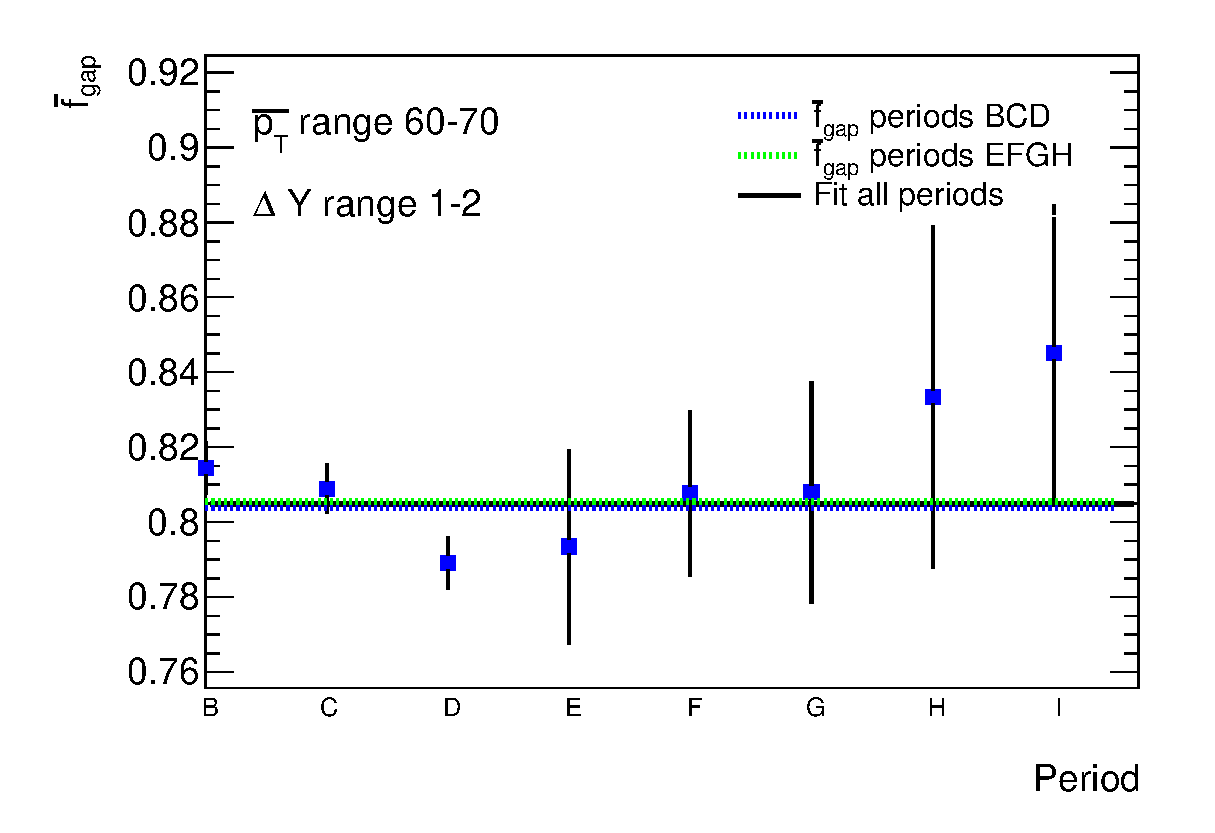
\includegraphics[width=\textwidth]{figures/GBJ1/DataStability/Pileup/GFAve_060_70_1-2_exclusive.eps}
        \end{subfigure}%
        \begin{subfigure}[b]{0.5\textwidth}
                \centering
                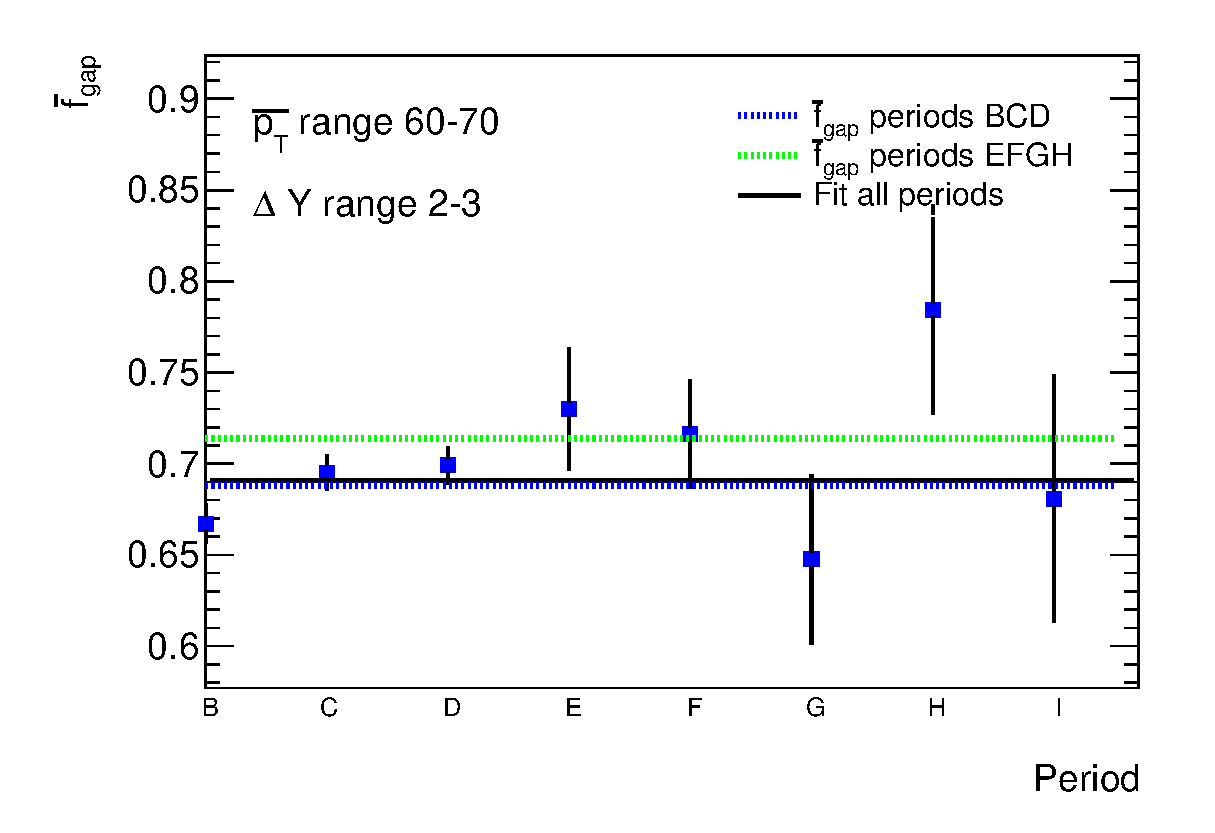
\includegraphics[width=\textwidth]{figures/GBJ1/DataStability/Pileup/GFAve_060_70_2-3_exclusive.eps}
        \end{subfigure}%

        \begin{subfigure}[b]{0.5\textwidth}
                \centering
                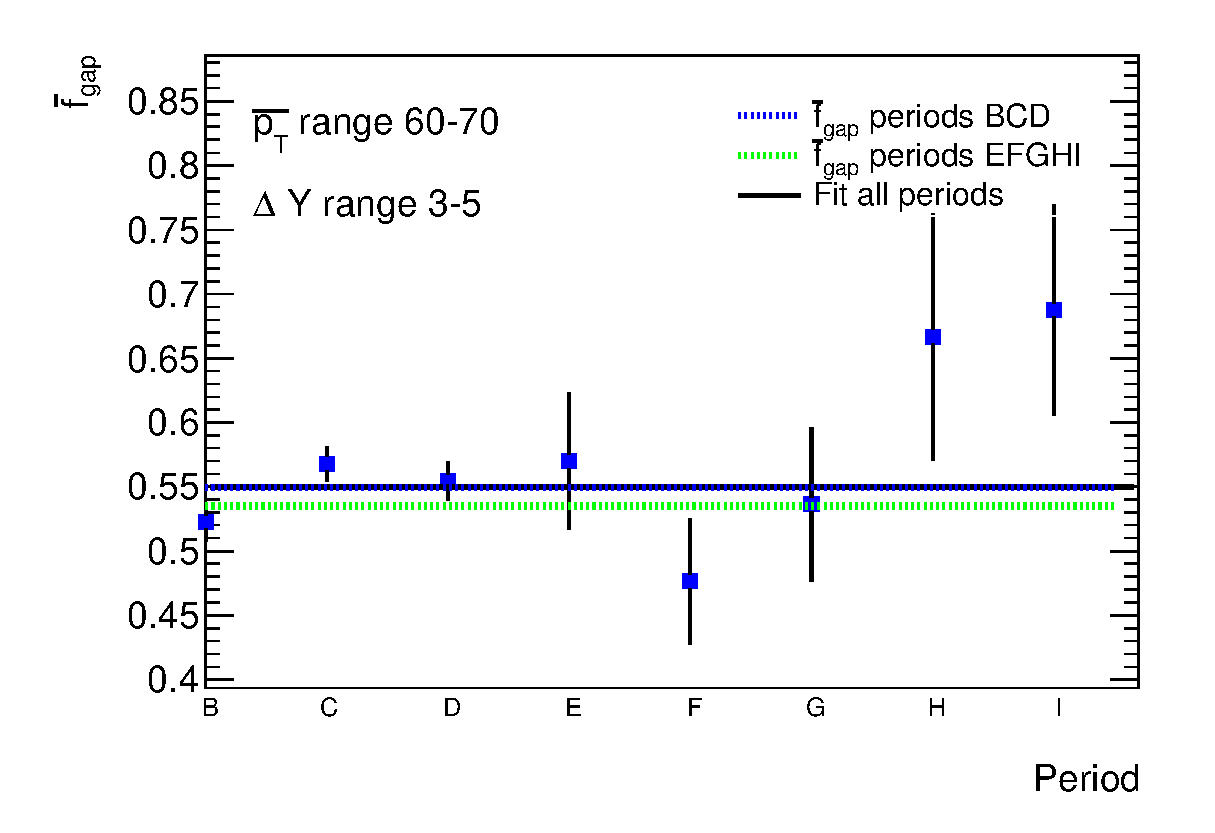
\includegraphics[width=\textwidth]{figures/GBJ1/DataStability/Pileup/GFAve_060_70_3-5_exclusive.eps}
        \end{subfigure}%

\caption[Average gap fraction versus period for $60<\ptb{}<70$ GeV]{
Average gap fraction with $60<\ptb{}<70$ GeV and (a) $1<\dy{}<2$, (b) $2<\dy{}<3$  and (c) $3<\dy{}<5$. 
Each set of average gap fractions have been fitted with three constants; one for periods B-D, one for periods E-I and one for all periods.
\label{GBJ1:GFAve6070}}
\end{figure}



\begin{figure}
\centering
        \begin{subfigure}[b]{0.5\textwidth}
                \centering
                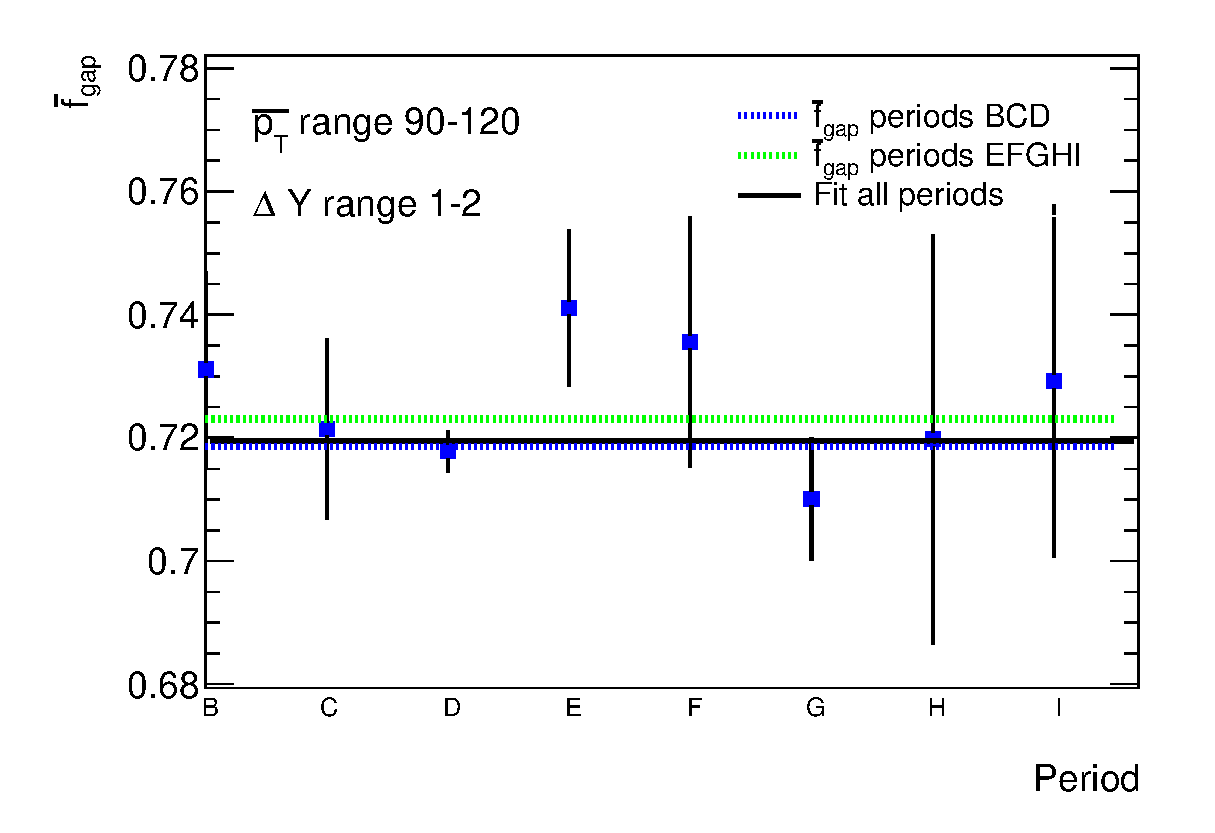
\includegraphics[width=\textwidth]{figures/GBJ1/DataStability/Pileup/GFAve_090_120_1-2_exclusive.eps}
        \end{subfigure}%
        \begin{subfigure}[b]{0.5\textwidth}
                \centering
                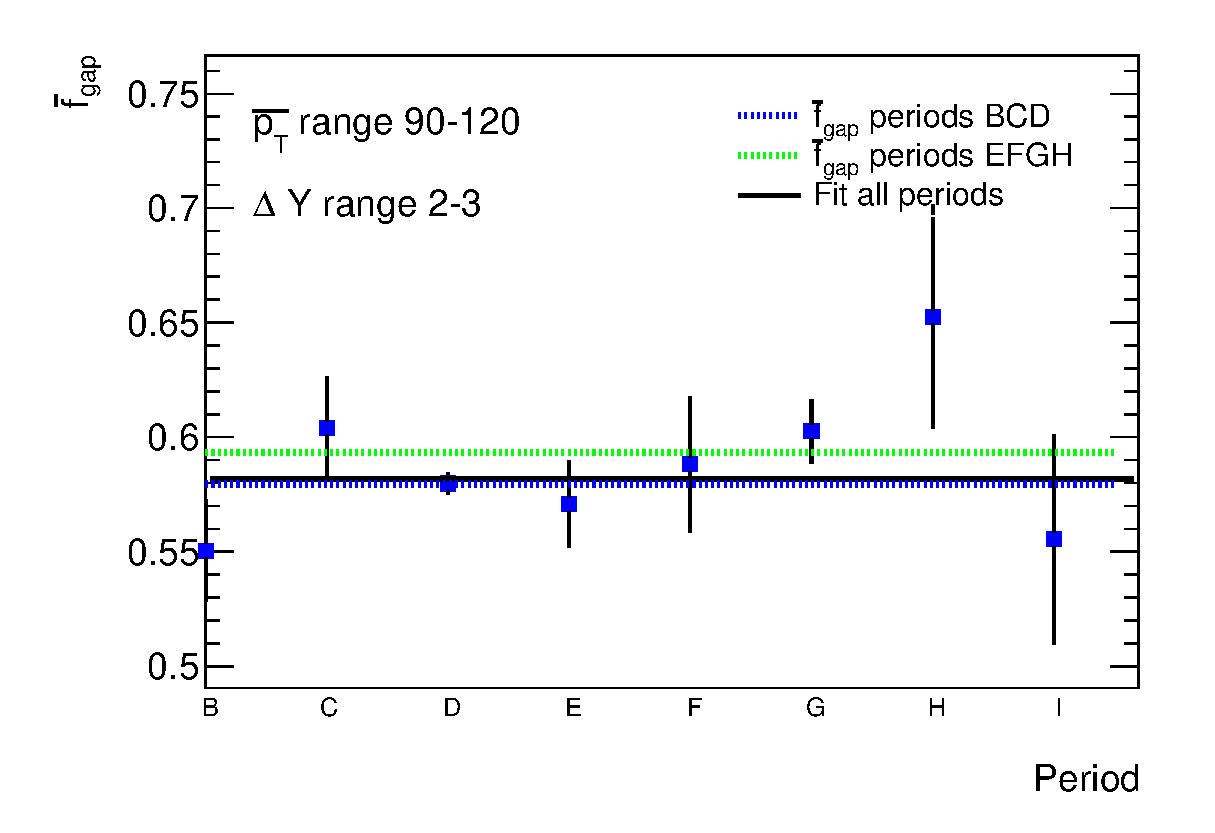
\includegraphics[width=\textwidth]{figures/GBJ1/DataStability/Pileup/GFAve_090_120_2-3_exclusive.eps}
        \end{subfigure}%

        \begin{subfigure}[b]{0.5\textwidth}
                \centering
                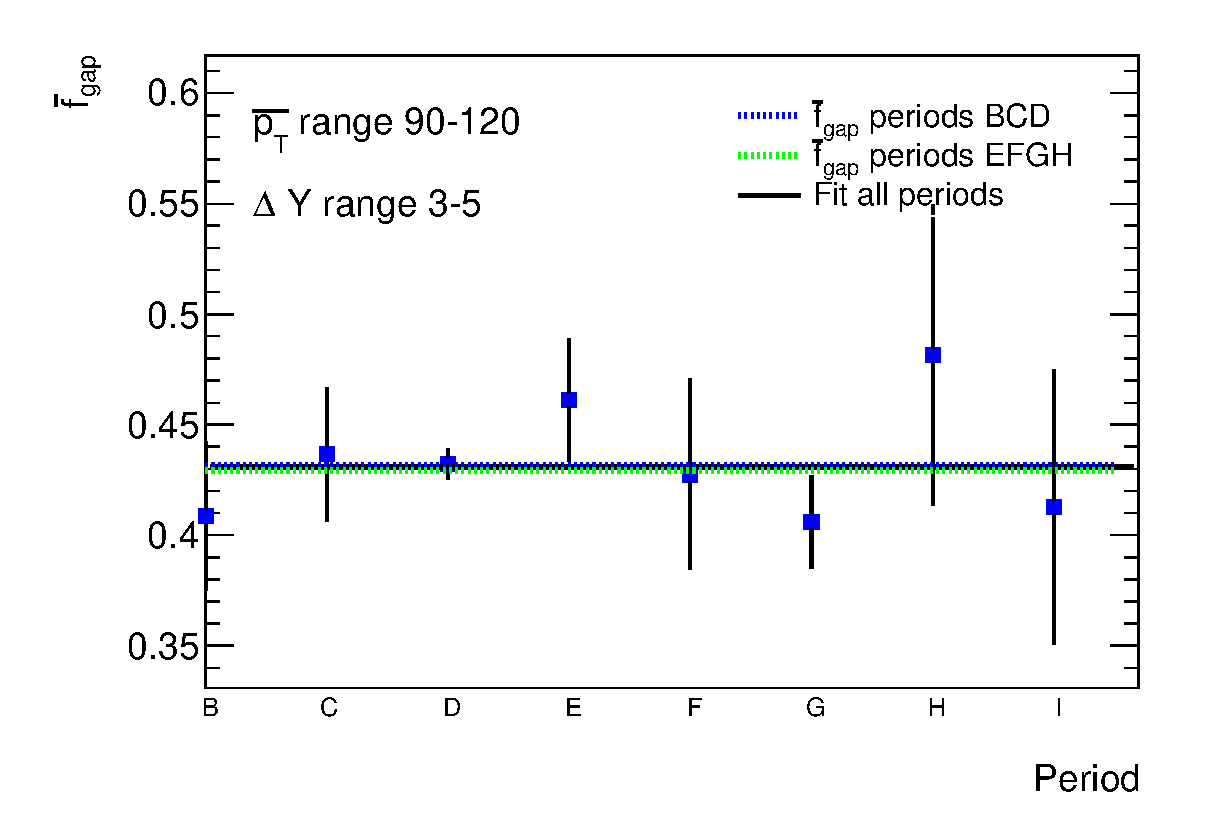
\includegraphics[width=\textwidth]{figures/GBJ1/DataStability/Pileup/GFAve_090_120_3-5_exclusive.eps}
        \end{subfigure}%
\caption[Average gap fraction versus period for $90<\ptb{}<120$ GeV]{
Average gap fraction with $90<\ptb{}<120$ GeV and (a) $1<\dy{}<2$, (b) $2<\dy{}<3$  and (c) $3<\dy{}<5$. 
Each set of average gap fractions have been fitted with three constants; one for periods B-D, one for periods E-I and one for all periods.
\label{GBJ1:GFAve90120}}
\end{figure}



\begin{figure}
\centering
        \begin{subfigure}[b]{0.5\textwidth}
                \centering
                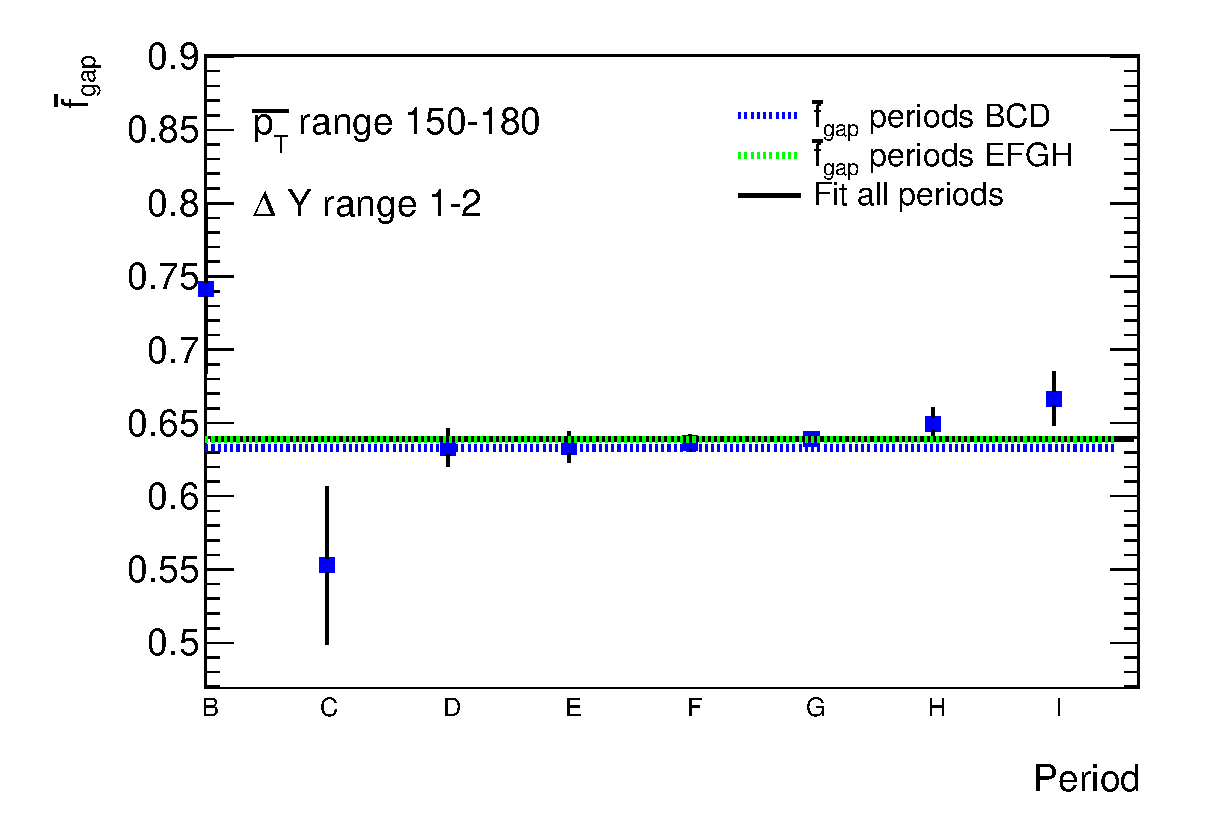
\includegraphics[width=\textwidth]{figures/GBJ1/DataStability/Pileup/GFAve_150_180_1-2_exclusive.eps}
        \end{subfigure}%
        \begin{subfigure}[b]{0.5\textwidth}
                \centering
                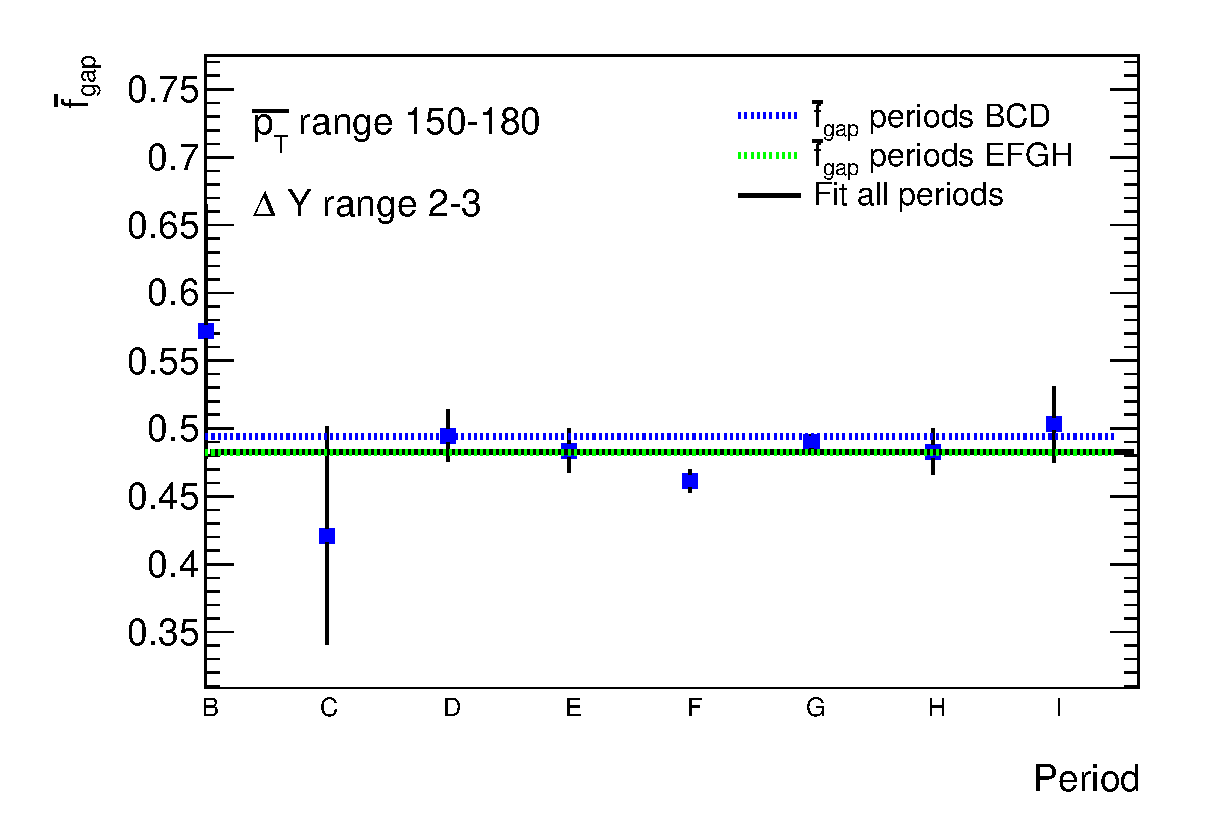
\includegraphics[width=\textwidth]{figures/GBJ1/DataStability/Pileup/GFAve_150_180_2-3_exclusive.eps}
        \end{subfigure}%

        \begin{subfigure}[b]{0.5\textwidth}
                \centering
                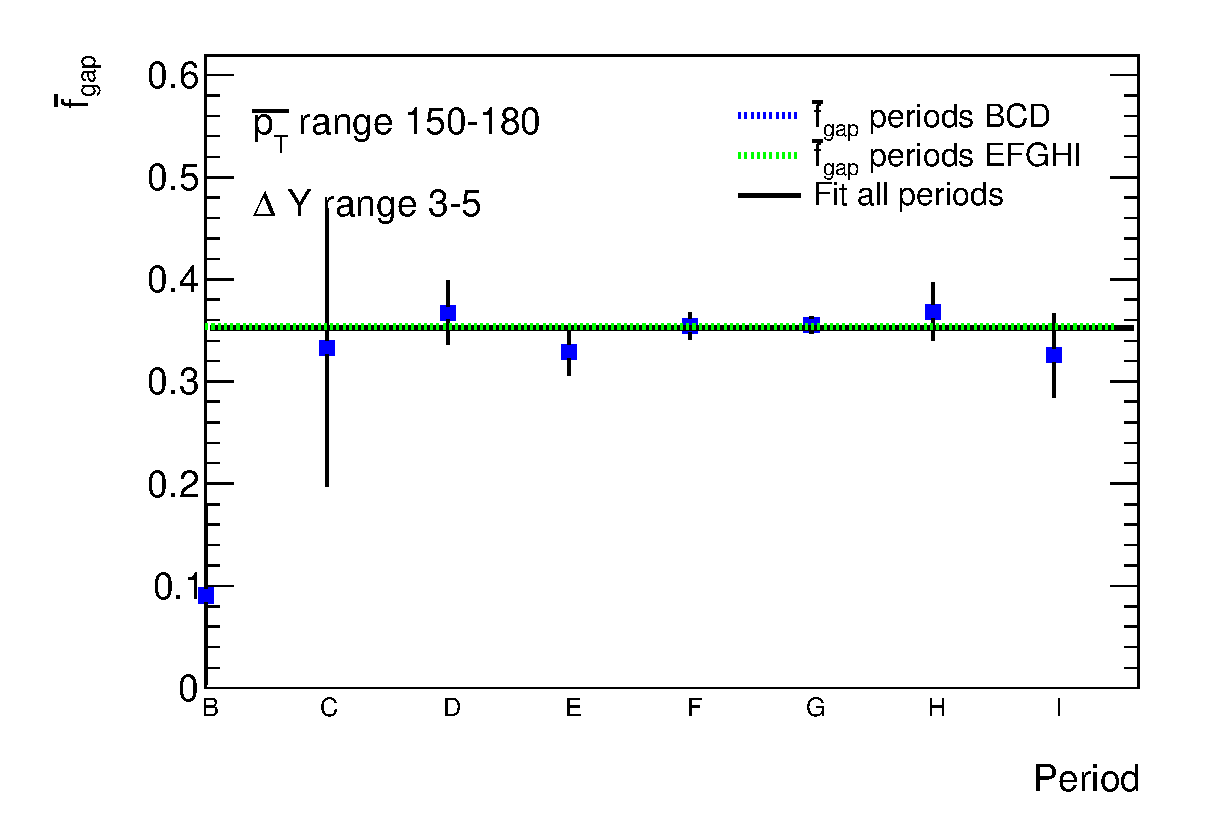
\includegraphics[width=\textwidth]{figures/GBJ1/DataStability/Pileup/GFAve_150_180_3-5_exclusive.eps}
        \end{subfigure}%
\caption[Average gap fraction versus period for $150<\ptb{}<180$ GeV]{
Average gap fraction with $150<\ptb{}<180$ GeV and (a) $1<\dy{}<2$, (b) $2<\dy{}<3$  and (c) $3<\dy{}<5$. 
Each set of average gap fractions have been fitted with three constants; one for periods B-D, one for periods E-I and one for all periods.
\label{GBJ1:GFAve150180}}
\end{figure}



\begin{table}
%\footnotesize 
%\small
\centering
\begin{tabular}{ | c | c | c | c | c | c |  }
\hline
\hline
\dy{} & \ptb{} & $\bar{f}_{gap}$ & \multicolumn{3}{|c|}{$y = A + Bx$}\\
   & GeV& Periods B-D &$A$&$B / 10^{-3}$&$\chi^{2}$/NDF\\
%\dy{} & $\ptb{} [GeV]$ & $\bar{f}_{gap}$ & b & c & d & e & f  \\
\hline
\input{figures/GBJ1/DataStability/Pileup/AveGFTable2.txt}
\hline
\hline
\end{tabular}
\caption[Results from period dependent and period independent fits to the average gap fraction as a function of period]{
The results from fits to the period dependent function in Equation \ref{GBJ1:Fit1} for various slices of \dy{} and \ptb{}.
\label{GBJ1:GFAveTable}}
\end{table}


\section{Overview of Other Analysis Components}
\label{sec:GBJ1:OtherWork}
To compare the data to theoretical models further aspects of the analysis were performed by other members of the analysis team. This section will dmension the unfolding of the data to hadron level. The systematic uncertainties in this analysis will then be discussed.

To compare the data to HEJ and POWHEG, detector and selection effects need to be accounted for, and the data needs to be unfolded back to hadron level. This was done using a bin-by-bin method comparing the final distributions from the PYTHIA sample at hadron and detector level. Rapidity weighted samples were generated and used to give good statistics in even the large $\Delta y$ regions.


The systematic uncertainties for various sources were considered. They were:
\begin{description}
\item[Jet Energy Scale (JES) uncertainty] varies depending on the $\Delta y$ bin. It can be as large at 5-10\% and is a significant source of uncertainty.

\item[Unfolding uncertainty] comes mainly from the limited statistics of the PYTHIA sample used to obtain the unfolding factors. It is a significant source of uncertainty with values as large as 5\%.

\item[Pileup] the effectiveness of the single primary vertex requirement, and the effect of out-of-time pileup was discussed in section \ref{sec:GBJ1:Pileup}. The average gap fraction was found to be unaffected by the change in pileup conditions, and so the effect from this is negligible.  

\item[Jet Cleaning Cuts] were changed to a stricter bad jet definition (which removed ~5\% of inclusive events) and there was a sub percent change to gap fraction distributions. This is negligble compared to the the uncertainty due to JES and unfolding.  

\item[Cosmic and beam backgrounds] event rates were estimated using triggers during non-filled bunch crossings. The rate of such evens was found to be very small compared to the rate of signal events, and the effect is taken to be negligible.

\item[Trigger Bias] was estimated by comparing the gap fraction and njets distributions with the analysis trigger strategy to the distributions obtained using the minimum bias stream and was found to be negligible in all regions.

\end{description}

The main two systematic uncertainties come from the JES and the unfolding. Figure \ref{GBJ1:SystUncert} shows the uncertainties from JES and unfolding and the combination for one $\Delta y$ and one $\bar{p_T}$ slice. The overall uncertainty does not change much with $\bar{p_T}$, but due to reduced statistics and moving into different regions of the detector both the JES, unfolding and overall uncertainty rise with larger $\Delta y$. For the final plots the overall systematic uncertainty and the statistical uncertainty have been added onto the data points.

\begin{figure}
\centering
\mbox{
              \subfigure[]{\epsfig{figure=figures/GBJ1/OtherWork/SystematicUncertainty_dY.eps,width=0.5\textwidth,height = 6cm}}\quad
              \subfigure[]{\epsfig{figure=figures/GBJ1/OtherWork/SystematicUncertainty_pT.eps,width=0.5\textwidth,height = 6cm}}\quad
                              }
\caption[Systematic uncertainty for the gap fraction for a slice in $\bar{p_T}$ and $\Delta y$]{Systematic uncertainty on the gap fraction versus (a) $\Delta y$ for $120<\bar{p_T}<150$ GeV and (b) $\bar{p_T}$ for $3<\Delta y<4$. 
\label{GBJ1:SystUncert}}
\end{figure}


\section{Corrected Data}
\label{sec:GBJ1:FinalPlots}

In this section, the final plots that were shown in the publication are discussed. 
The plots shown are from  the leading \pt{} dijet selection and the forward/backwards selection and show the gap fraction as a function of \dy{}, \ptb{} and \qz{}, and also the mean number of jets in the rapidity interval as a function of \dy{} and \ptb{}. 
When \dy{} and \ptb{} are studied, \qz{} is always at a fixed value of 20 GeV. 
The data is sliced into different regions. 
The gap fraction and mean number of jets versus \dy{} distributions are shown for seven different \ptb{} ranges, and it is shown versus \ptb{} for five different \dy{} ranges. 
Each slice is offset to allow the data to be shown on one plot. 
The ratio of the theory predictions to data is shown next to each plot.

On each plot, the black points are the data points with statistical uncertainty bars, with the yellow bands indicating the systematic uncertainty from both the JES and unfolding. 
The red and blue dotted lines are the POWHEG + PYTHIA and POWHEG + HERWIG predictions respectively, and the blue band is the HEJ prediction with a theoretical uncertainty.

Figures \ref{GBJ1:dYSelA} and \ref{GBJ1:pTSelA} show the gap fraction and the ratio of theory to data as a function of $\dy{}$ and $\ptb{}$, respectively, for different \ptb{} and \dy{} slices for the leading \pt{} dijet selection. 
The gap fraction from the data reduces as a function of \ptb{} and \dy{}.
When the rapidity region between the dijets is small, the phase space for emission is small. 
When the \dy{} or the \ptb{} of the dijets increases, the phase space available for emission increase, and so the gap fraction decreases.
For the highest \ptb{} range, the gap fraction starts to level off. 
This feature could be due to PDF effects, where both of the jets have high \pt{}, and so the probability of having another jet in the event is low.
HEJ agrees well with the data for the complete range in $\dy$ for low $\ptb{}$. 
However, for $\ptb{}$ slices $150\le\ptb{}<180$ GeV and above, HEJ starts to overestimate the gap fraction.
This deviation is shown more clearly as a function of \ptb{}.
HEJ deviates from the data for $\ptb{}>140$ GeV for all but the highest \dy{} slices, in which there are significant uncertainties.
As described in Section \ref{Theory:MC}, HEJ is relevant only for hard wide angle emissions.
Therefore, is it not unexpected that it should do better when $\qz{}\approx\ptb{}$, and to do worse when $Q_{0}<<\ptb{}$.

POWHEG + PYTHIA and POWHEG + HERWIG give significantly different gap fractions as a function of \dy{} and \ptb{}.
POWHEG + PYTHIA gives the best overall description of the data.
POWHEG + PYTHIA agrees with the data at all \ptb{} slices for low \dy{}, however it starts to deviate for $\dy{}>3.5$. 
This can also be seen for the gap fraction as a function of \ptb{} for the different \dy{} slices. 
For the slices, $1\le\dy{}<2$, $2\le\dy{}<3$, and $3\le\dy{}<4$, the agreement is very good throughout \ptb{}, with only deviations away from the data at large \dy{} which correspond to statistical fluctuations.
However, for the other \dy{} slices POWHEG + PYTHIA gives too low a gap fraction.
Conversely, POWHEG + HERWIG only agrees with the data only in the lowest of \dy{} bins, it deviates for $\dy{}>1$ for all slices of \ptb{}. 
In the gap fraction against \ptb{} for different \dy{} slices distributions, POWHEG + HERWIG does not agree well with the data and underestimates the gap fraction for all considered regions of phase space.
The difference between POWHEG + PYTHIA and POWHEG + HERWIG is an indication of the uncertainty in current calculations of parton showers.


Figure \ref{GBJ1:Q0SelA} shows the gap fraction as a function of \qz{} for different slices in \dy{} and \ptb{} for the leading \pt{} dijet selection.
For a low \qz{} value, the gap fraction is at a minimum, as any increase in \qz{} will reduce the number of events with a jet above \qz{}.
When the \qz{} increases the gap fraction increases, which is expected as the probability of getting a very high \pt{} emission is lower.
POWHEG + HERWIG underestimates the data for all but the highest \qz{} bins, indicating that there is too much emission from the POWHEG + HERWIG parton shower. 
For the gap fraction against \qz{} for $2\le\dy{}<3$ and  $70\le\pt{}<90$ GeV slice, both HEJ and POWHEG + PYTHIA overlaps with the data throughout the \qz{} range. 
For the other slices, at low \qz{} HEJ overestimates the gap fraction, but improves as $\qz{}\approx\ptb{}$, which is expected as HEJ generates partons with similar \pt{}.
Neither POWHEG + PYTHIA or HEJ agrees well with the gap fraction when both \dy{} and \qz{} is large.



Figures \ref{GBJ1:NjetsdYSelA} and \ref{GBJ1:NjetspTSelA} are the mean number of jets in the rapidity interval between the boundary jets as a function of $\dy{}$ and $\ptb{}$, respectively, for slices in \ptb{} and \dy{} for the leading \pt{} dijet selection. 
This is an alternative method of probing the activity between the boundary jets. 
The gap fraction is only concerned with the leading jet in the rapidity region, but the average number of jets considers all jet in that region with a $\pt{}>20$ GeV. 
As with the gap fraction, POWHEG + PYTHIA agrees best with the data.
POWHEG + HERWIG consistently gives too much activity in the rapidity region, which helps to explain why the POWHEG + HERWIG gap fraction is below the data.
Except at very low \ptb{}, HEJ has too little activity in the rapidity region.
Comparing to the gap fraction slices, in which it agrees with data, would indicate that HEJ describes only the highest \pt{} emission between the dijet well. 

 
Figures \ref{GBJ1:dYSelB} and \ref{GBJ1:pTSelB} show the gap fraction and the ratio of theory to data as a function of $\dy{}$ and $\ptb{}$, respectively, for different \ptb{} and \dy{} slices for the forward/backward dijet selection.
For this selection, there are often imbalances in the \pt{} of the boundary jets, especially at larger \ptb{}.
All three model comparisons show similar difference to the data. 
The gap fraction from HEJ as a function of \dy{} falls below the data for low \ptb{} slices. 
It has been suggested in \cite{ref:Anderson1} that this is due to the importance of soft emission from the dijets.

Figure \ref{GBJ1:Q0SelB} shows the gap fraction as a function of \qz{} for different slices in \dy{} and \ptb{} for the forward/backward dijet selection.
In the leading \pt{} dijet selection, the maximum \pt{} of a jet in the rapidity region between the dijet system is the \pt{} of the subleading jet (which has a maximum \pt{} of \ptb{}).
Above the \ptb{} of the jet, the gap fraction must be one.
However, for the forward/backward dijet selection, the \pt{} of a jet in the rapidity region between the dijet system is less affected by the \ptb{}.
The gap fraction does not rise as quickly as in the previous selection.
The POWHEG + PYTHIA  shows similar agreement to the data as for the previous selection.
HEJ does not agree well with the data, and especially for the higher \dy{} slices, it has a consistently low gap fraction throughout \qz{}. 

Figure \ref{GBJ1:pTSelBQ0} shows the gap fraction as a function of $\dy{}$ and $\ptb{}$ respectively for different \ptb{} and \dy{} slices for the forward/backward dijet selection, but the \qz{} is set to the \ptb{} of the event. 
This shows how the gap fraction is affected by emissions which are harder than the \ptb{} of the  dijets. 
POWHEG + PYTHIA and POWHEG + HERWIG both overlap the data.
This would indicate that this definition of the gap fraction is less dependent on the modelling of the parton shower, hadronisation and underlying event.
The new definition of the jet veto does not improve the HEJ agreement with the data.


Since publishing the results of this analysis, several papers \cite{ref:Anderson1,ref:JeffNew} have compared  their theoretical predictions to the ATLAS data. 
Both discuss the unreliability of fixed order calculations in this topology of event.
Reference \cite{ref:JeffNew} uses an all-order resummation in $\ln(\pt{}/\qz{})$ terms to compare to the data, observing a large theoretical uncertainty. 
The conclusion of the paper is: ``The message is clear: the accuracy of the ATLAS data already demands better theoretical calculations''.


\begin{figure}
\centering
        \centering
        \begin{subfigure}[b]{0.3\textwidth}
                \centering
                \epsfig{figure=figures/GBJ1/FinalData/GF_dY.eps,width=0.45\textwidth}
                \caption{A gull}
                \label{fig:gull}
        \end{subfigure}%
        \begin{subfigure}[b]{0.3\textwidth}
                \centering
                \epsfig{figure=figures/GBJ1/FinalData/GF_dY_ratio.eps,width=0.45\textwidth}
                \caption{A tiger}
                \label{fig:tiger}
        \end{subfigure}
\end{figure}
\mbox{
              \subfigure[]{\epsfig{figure=figures/GBJ1/FinalData/GF_dY.eps,width=0.45\textwidth}}
              \subfigure[]{\epsfig{figure=figures/GBJ1/FinalData/GF_dY_ratio.eps,width=0.45\textwidth}}
}
\mbox{
              \subfigure[]{\epsfig{figure=figures/GBJ1/FinalData/GF_dY.eps,width=0.45\textwidth}}
              \subfigure[]{\epsfig{figure=figures/GBJ1/FinalData/GF_dY_ratio.eps,width=0.45\textwidth}}
}
\caption[Gap fraction as a function of  \dy{} for the leading \pt{} dijet selection]{
(a) Gap fraction as a function of \dy{} for various \ptb{} slices for the leading \pt{} dijet selection. 
(b) Ratio between the theoretical predictions and the data.
\label{GBJ1:dYSelA}}
\end{figure}



\begin{figure}
\centering
\mbox{
              \subfigure[]{\epsfig{figure=figures/GBJ1/FinalData/GF_ptBar.eps,width=0.5\textwidth}}\quad
              \subfigure[]{\epsfig{figure=figures/GBJ1/FinalData/GF_ptBar_ratio.eps,width=0.5\textwidth}}\quad
}
\caption[Gap fraction as a function of \ptb{} for leading \pt{} dijet selection]{ 
(a) Gap fraction as a function of \ptb{} for various \dy{} slices for the leading \pt{} dijet selection. 
(b) Ratio between the theoretical predictions and data.
\label{GBJ1:pTSelA}}
\end{figure}



\begin{figure}
\centering
\mbox{
              \subfigure[]{\epsfig{figure=figures/GBJ1/FinalData/GF_Q0.eps,width=0.5\textwidth}}\quad
              \subfigure[]{\epsfig{figure=figures/GBJ1/FinalData/GF_Q0_ratio.eps,width=0.5\textwidth}}\quad
}
\caption[Gap fraction as a function of \qz{} for leading \pt{} dijet selection]{ 
(a) Gap fraction as a function of \qz{} for various \dy{} and \ptb{} slices for the leading \pt{} dijet selection. 
(b) Ratio between the theoretical predictions and data. 
\label{GBJ1:Q0SelA}}
\end{figure}

\begin{figure}
\centering
\mbox{
              \subfigure[]{\epsfig{figure=figures/GBJ1/FinalData/GF_Njets_dY.eps,width=0.5\textwidth}}\quad
              \subfigure[]{\epsfig{figure=figures/GBJ1/FinalData/GF_Njets_dY_ratio.eps,width=0.5\textwidth}}\quad
}
\caption[Mean number of jets as a function of \dy{} for leading \pt{} dijet selection]{ 
(a) Mean number of jets in the rapidity region bounded by the dijet system as a function of \dy{} for various \ptb{} slices for the leading \pt{} dijet selection. 
(b) Ratio between the theoretical predictions and data. 
\label{GBJ1:NjetsdYSelA}}
\end{figure}

\begin{figure}
\centering
\mbox{
              \subfigure[]{\epsfig{figure=figures/GBJ1/FinalData/GF_Njets.eps,width=0.5\textwidth}}\quad
              \subfigure[]{\epsfig{figure=figures/GBJ1/FinalData/GF_Njets_ratio.eps,width=0.5\textwidth}}\quad
}
\caption[Mean number of jets as a function of \ptb{} for leading $p_T$ dijet selection]{ 
(a) Mean number of jets in the rapidity region bounded by the dijet system as a function of \ptb{} for various \dy{} slices for the leading \pt{} dijet selection. 
(b) Ratio between the theoretical predictions and data.
\label{GBJ1:NjetspTSelA}}
\end{figure}

%%%%%%%%%%%%%%%%%%%SELECTION B%%%%%%%%%%%%%%%%%%%%%%

\begin{figure}
\centering
\mbox{
              \subfigure[]{\epsfig{figure=figures/GBJ1/FinalData/GF_dY_SelB.eps,width=0.5\textwidth}}\quad
              \subfigure[]{\epsfig{figure=figures/GBJ1/FinalData/GF_dY_SelB_ratio.eps,width=0.5\textwidth}}\quad
}
\caption[Gap fraction as a function of \dy{} for forward backward selection]{ 
(a) Gap fraction as a function of \dy{} for various \ptb{} slices for the forward backward selection. 
(b) Ratio between the theoretical predictions and data. 
\label{GBJ1:dYSelB}}
\end{figure}

\begin{figure}
\centering
\mbox{
              \subfigure[]{\epsfig{figure=figures/GBJ1/FinalData/GF_SelB_pT.eps,width=0.5\textwidth}}\quad
              \subfigure[]{\epsfig{figure=figures/GBJ1/FinalData/GF_SelB_pT_ratio.eps,width=0.5\textwidth}}\quad
}
\caption[Gap fraction as a function of \ptb{} for forward backward selection]{ 
(a) Gap fraction as a function of \ptb{} for various \dy{} slices for the forward backward selection. 
(b) Ratio between the theoretical predictions and data.
\label{GBJ1:pTSelB}}
\end{figure}

\begin{figure}
\centering
\mbox{
              \subfigure[]{\epsfig{figure=figures/GBJ1/FinalData/GF_SelB_Q0.eps,width=0.5\textwidth}}\quad
              \subfigure[]{\epsfig{figure=figures/GBJ1/FinalData/GF_SelB_Q0_ratio.eps,width=0.5\textwidth}}\quad
}
\caption[Gap fraction as a function of \qz{} for forward backward selection]{ 
(a) Gap fraction as a function of \qz{} for various \dy{} and \ptb{} slices for the forward backward selection. 
(b) Ratio between the theoretical predictions and data. 
\label{GBJ1:Q0SelB}}
\end{figure}


\begin{figure}
\centering
\mbox{
              \subfigure[]{\epsfig{figure=figures/GBJ1/FinalData/GF_SelB_dY_Q0pTbar.eps,width=0.5\textwidth}}\quad
              \subfigure[]{\epsfig{figure=figures/GBJ1/FinalData/GF_SelB_dY_Q0pTbar_ratio.eps,width=0.5\textwidth}}\quad
}
\caption[Gap fraction as a function of \dy{} for forward backward selection and variable \qz{}]{ 
(a) Gap fraction as a function of \dy{} for various \ptb{} slices for the forward backward selection with veto scale set as \ptb{}. 
(b) Ratio between the theoretical predictions and data. 
\label{GBJ1:pTSelBQ0}}
\end{figure}





\chapter{Dijets with a Jet Veto and Azimuthal Decorrelations at Very Large Rapidity Separations}
\label{chp:GBJ2}
The first LHC measurement of dijet production with a jet veto (documented in Chapter \ref{chp:GBJ1} and \cite{ref:ATLASGap}) examined the gap fraction in slices \ptb{} up to $\dy{}=6$.
This cut-off in \dy{} is necessary because the analysis uses a central jet trigger strategy in which the trigger fires if a jet is within $|y|<2.8$.
There is a relatively small number of events at large \dy{} where the statistical uncertainties are large. 
The data are compared to theory predictions by HEJ and POWHEG.

The analysis is extended to probe the gap fraction at a larger \dy{} region.
This larger \dy{} region is again studied using the 2010 data, but using a new dijet trigger strategy that allowes measurements up to $\dy{}=8$, which is the boundary of the detector.
In addition, the effect of quark/gluon emission from the dijet system is studied using the azimuthal decorrelation between the jets that make up the dijet system.
The previous ATLAS measurement of azimuthal decorrelation was carried out using jets with an $|\eta{}| < 0.8$ \cite{ref:Decorr}.


\section{Topology Selection}
\label{sec:GBJ2:AnalSel}
The jets used in this analysis were reconstructed from EM scale calorimeter clusters with the anti$-k_T$ algorithm, described in Section \ref{sec:Theory:Jets}, using a radius parameter R=0.6.
As for the previous analysis, jets that have \pt{}$>20$ GeV and $|y|<4.4$ are used, as these have a well defined jet energy scale and jet cleaning cuts.
The dijet system is defined by the two leading jets in the event, with cuts on the transverse momentum of the leading and sub-leading jets of $\pt{}>60$ GeV and $\pt{}>50$ GeV, respectively.



The observables studied can loosely be divided into azimuthal decorralation observables, and jet veto observables.
The jet veto observables are the same as defined in the previous chapter, where the gap fraction, \gap{}, is defined by,
\begin{equation}
f_{\rm gap} = \frac{n (\qz{})}{N},
\label{GBJ2:fgap}
\end{equation}
where n(\qz{}) is the number of gap events which pass the jet veto, with scale \qz{}, and $N$ is the inclusive number of events.
The gap fraction is studied as a function of \dy{} and \qz{}.
Again the mean number of jets found in the rapidity region between the dijets \nb{} that have \pt{}$>$\qz{} is also studied. 
The azimuthal decorralation variables are
\begin{equation}
\frac{d\sigma}{d\Delta\phi},~\mean{\cosdphi}~\rm{and}~\mean{\costwodphi}.
\label{GBJ2:AZVar}
\end{equation}
The cross section as a function of \dphi{} is measured in slices of \dy{}.
The average decorrelation variables (\mean{\cosdphi} and \mean{\costwodphi})  are studied as a function of \dy{}
All decorrelation variables are studied separately for inclusive and gap events (those that survive a jet veto).
The standard jet veto scale that is used to define gap events is $\qz{}=20$ GeV.



\section {Event selection}
\label{sec:GBJ2:EvtSel}
\subsection{Data Samples and Basic Event Selection}
The analysis is performed using pp collisions at $\sqrt{s}=7$ TeV, recorded between April and October 2010 using the ATLAS detector.
Stable beam conditions and good data quality is required; the data quality was assessed by the ATLAS performance working groups by checking that all the parts of the detector and trigger were performing normally, and the physics objects (for instance jets and muons) were being correctly reconstructed. 
Events are rejected if there is any jet with $p_T>20$ GeV that is found as either bad or ugly as described in Section \ref{sec:Det:Jets}. 
Events are also rejected if the number of reconstructed primary vertices is not equal to one.


\subsection{Trigger Strategy}

For each of the two leading offline jets, a specific trigger chain is assigned depending on the rapidity $y$ and \pt{} of the offline jet as well as the run number.
Tables \ref{tab:CentralTrigger}, \ref{tab:TransTrigger} and \ref{tab:ForwardTrigger} show the trigger chains assigned to jets in the central ($|y|<2.9$), forward transition ($3.3\le|y|<3.6$) and forward trigger regions ($3.6\le|y|<4.4$), respectively.
If a jet falls into the region $2.9\le|y|<3.3$, the offline jet is matched to the closest L1 trigger jet using $\dr{}=\sqrt{(\dphi{})^2 + (\deta{})^2}$.
It is defined as a central (forward) jet  if it is closest to a trigger jet that fired a central (forward) jet trigger, and the trigger chain is subsequently defined using Table \ref{tab:CentralTrigger} (Table \ref{tab:TransTrigger}).
Either of the trigger chains associated with the leading jets are required to fire for the event to pass.

This trigger strategy has previously been used in the measurement of the dijet cross-section \cite{ref:Dijet}.
In most regions of phase space, the trigger efficiency for each considered jet is $100\%$.
However, there are two regions in which that is not the case.
The first is the crack region, $1.3\le|y|\le1.6$, between the barrel and end-cap calorimeter.
The second is in the positive FCAL region in which there is a dead trigger tower that reduces the trigger efficiency for jets with $|y|>3.1$.
For each jet that falls into one of these regions, the event is weighted by 
\begin{equation}
W_{eff}= \frac{\mathcal{P}_{lead}}{\epsilon_{lead}} + \frac{\mathcal{P}_{sublead}}{\epsilon_{sublead}} -\frac{\mathcal{P}_{lead}\mathcal{P}_{sublead}}{\epsilon_{lead}\epsilon_{sublead}}
\label{GBJ2:Eff}
\end{equation}
where $\mathcal{P}_{lead}$ and $\mathcal{P}_{sublead}$ is 1 if the event passed the leading and subleading trigger chain, else it is zero, and $\epsilon_{lead}$ and $\epsilon_{sublead}$ are their \pt{} dependent efficiencies for the leading and subleading jets.
The efficiencies are taken from the analysis in~\cite{ref:Dijet}.

During data taking, prescales are applied to the jet trigger to preferentially select events with higher \pt{} jets; only the highest \pt{} trigger is unprescaled.
The end result is a flattening of the jet \pt{} spectrum.
To retrieve the original distribution, the events are weighted by the inverse of an effective luminosity for each trigger combination.
The effective luminosity is calculated by
\begin{equation}
\mathcal{L}_{eff} = \sum_{LB} \frac{\mathcal{L}_{LB}}{P_{LB}^L P_{LB}^{SL}/(P_{LB}^L + P_{LB}^{SL} -1)}
\label{GBJ2:LBeff}
\end{equation}
where $P_{LB}^L$ and $P_{LB}^{SL}$ are the prescales for a given luminosity for the trigger chain associated with the leading and subleading jet, respectively, and $\mathcal{L}_{LB}$ is the luminosity for the luminosity block. 

The effective luminosities were calculated in \cite{ref:Dijet} for all pile-up conditions.
In this analysis, a single vertex cut is applied, which effectively reduces the luminosity $\mathcal{L}_{LB}$ in Equation \ref{GBJ2:LBeff} by a factor $f_{L}$.
A single vertex correction is derived for this analysis, defined as 
\begin{equation}
 f_{L} = \frac{N_{SV}}{N_{ALL}},
\label{GBJ2:SVCorrection}
\end{equation}
where $N_{SV}$ is the number of events with only one vertex and  $N_{ALL}$ is the total number of events, for every trigger combination.
The effective luminosity, $\mathcal{L}_{eff}$, is then weighted by $f_{L}^{-1}$ to return the correct luminosity for the measurement.

\begin{table}[htdp]
\centering
\begin{tabular}{ | c | c | c | c | }
  \hline
 \pt{} [GeV] & Period A-C & Period D-F & Period G-I \\
  \hline
20--42.5 &  $ \rm L1\_ MBTS\_ 1$ & $ \rm L1\_ MBTS\_ 1$ & $ \rm EF\_ mbMbts\_ 1\_ eff$  \\
42.5--70 &  $ \rm L1\_ J5$ &     $ \rm L1\_ J5$ &     $ \rm EF\_ j20\_ jetNoEF$  \\
70--97.5 &   $ \rm L1\_ J15$ &    $ \rm L1\_ J15$ &    $ \rm EF\_ j35\_ jetNoEF$  \\
97.5--152.5 &   $ \rm L1\_ J30$ &    $ \rm L1\_ J30$ &    $ \rm EF\_ j50\_ jetNoEF$  \\
152.5--197.5 &  $ \rm L1\_ J55$ &    $ \rm L1\_ J55$ &    $ \rm EF\_ j75\_ jetNoEF$  \\
197.5--217.5 &  $ \rm L1\_ J55$ &    $ \rm L1\_ J55$ &    $ \rm EF\_ j95\_ jetNoEF$  \\
217.5+ &     $ \rm L1\_ J55$ &    $ \rm L1\_ J55$ &    $ \rm EF\_ L1J95\_ NoAlg$ \\

  \hline
\end{tabular}
\caption[Triggers used for jets in the central region]{
Trigger chains used for central trigger region, $|y|<2.9$, for jet \pt{} and period.
\label{tab:CentralTrigger}}
\end{table}%


\begin{table}[htdp]
\centering
\begin{tabular}{ | c | c | c | c | }
\hline
\pt{} [GeV] & Period A-D  & Period E-F & Period G-I \\
      \hline
         20--42.5 &     $ \rm L1\_ MBTS\_ 1$ & $ \rm L1\_ MBTS\_ 1$  &   $ \rm EF\_ mbMbts\_ 1\_ eff$  \\
         42.5--62.5 &   $ \rm L1\_ MBTS\_ 1$ & $ \rm L1\_ FJ10$      &   $ \rm EF\_ mbMbts\_ 1\_ eff$  \\
         62.5--72.5 &   $ \rm L1\_ MBTS\_ 1$ & $ \rm L1\_ FJ10$      &   $ \rm EF\_ fj30\_ jetNoEF$  \\
         72.5--95 &     $ \rm L1\_ MBTS\_ 1$ & $ \rm L1\_ FJ30$      &   $ \rm EF\_ fj30\_ jetNoEF$  \\
         95--160 &      $ \rm L1\_ MBTS\_ 1$ & $ \rm L1\_ FJ30$      &   $ \rm EF\_ fj50\_ jetNoEF$  \\
         160+ &         $ \rm L1\_ MBTS\_ 1$ & $ \rm L1\_ FJ30$      &   $ \rm EF\_ fj75\_ jetNoEF$  \\
         \hline
      \end{tabular}
\caption[Triggers used for jets in the transition region]{
      Trigger chains used for transition trigger region, $3.3\le|y|<3.6$, for jet \pt{} and period.
      \label{tab:TransTrigger}}
\end{table}%

\begin{table}[htdp]
\centering
\begin{tabular}{ | c | c | c | c | }
  \hline
 \pt{} [GeV] & Period A-D & Period E-F & Period G-I \\
  \hline
\rm 20--42.5 &       $\rm L1\_ MBTS\_ 1$ & $\rm L1\_ FJ10$ & $\rm EF\_ mbMbts\_ 1\_ eff$  \\
\rm 42.5--50 &       $\rm L1\_ MBTS\_ 1$ & $\rm L1\_ FJ10$ & $\rm EF\_ fj30\_ jetNoEF$  \\
\rm 50--67.5 &       $\rm L1\_ MBTS\_ 1$ & $\rm L1\_ FJ30$ & $\rm EF\_ fj30\_ jetNoEF$  \\
\rm 67.5--100 &      $\rm L1\_ MBTS\_ 1$ & $\rm L1\_ FJ30$ & $\rm EF\_ fj50\_ jetNoEF$  \\
\rm 100+ &           $\rm L1\_ MBTS\_ 1$ & $\rm L1\_ FJ30$ & $\rm EF\_ fj75\_ jetNoEF$  \\

  \hline
\end{tabular}
\caption[Triggers used for jets in the forward region]{
Trigger chains used for forward trigger region, $3.6\le|y|<4.4$, for jet \pt{} and period.
\label{tab:ForwardTrigger}}
\end{table}%

 
\section{Closure of Event Selection}
\label{sec:GBJ2:AODD3PD}

To check the event selection, two separate implementations of the analysis were performed by the Manchester and UCL groups and the the agreement of the final plots checked.
One of these analyses was carried out using the ATLAS AOD data format, whilst the other used the ATLAS D3PD format.
Figure \ref{GBJ2:AODD3PD:gap_njet} shows (a) the  gap fraction and (b) the  average number of jets in the rapidity region as a function of \dy{}.
Figure \ref{GBJ2:AODD3PD:dphi} shows the \dphi{} distribution for inclusive events for a dijet separation, \dy{}, of (a) 2-3 and (b) 4-5. 
All four plots show very good agreement between the AOD and D3PD implementations of the analysis.
The small disagreements arise from the data compression algorithms that store the data information.
This effects mainly the jet energies and the effect is much smaller than the JES uncertainty.


\begin{figure}
\centering
\mbox{
              \subfigure[]{\epsfig{figure=figures/GBJ2/AODD3PD/Comp_GapFraction_deltaY.eps,width=0.5\textwidth,height = 6cm}}\quad
              \subfigure[]{\epsfig{figure=figures/GBJ2/AODD3PD/Comp_prof_deltaY_njets.eps,width=0.5\textwidth,height = 6cm}}\quad
                              }
\caption[]{
(a) Gap fraction and (b) average number of jets in the rapidity region as a function of dijet separation, \dy{}, for 2010 uncorrected data from the AOD (red) and D3PD (black) data formats.
\label{GBJ2:AODD3PD:gap_njet}}
\end{figure}


\begin{figure}
\centering
\mbox{
              \subfigure[]{\epsfig{figure=figures/GBJ2/AODD3PD/Comp_dPhi__2_3-Edit.eps,width=0.5\textwidth,height = 6cm}}\quad
              \subfigure[]{\epsfig{figure=figures/GBJ2/AODD3PD/Comp_dPhi__4_5-Edit.eps,width=0.5\textwidth,height = 6cm}}\quad
                              }
\caption[]{
\dphi{} distribution for inclusive events for a dijet separation, \dy{}, of (a) 2-3 and (b) 4-5 for 2010 uncorrected data from the AOD (red) and D3PD (black) data formats.
\label{GBJ2:AODD3PD:dphi}}
\end{figure}


\section{Systematic Uncertainty}
\label{GBJ2:system}

In this section, the systematic uncertainties from the jet cleaning cuts, jet energy scale uncertainty, jet energy resolution and jet $\phi$ resolution are assessed.
These uncertainties are added in quadrature with other uncertainties calculated by other members of the analysis team. 



\subsection{Jet Energy Scale Uncertainty}

The effect of the JES is studied using the rapidity weighted PYTHIA samples.
Each jet, which is at the central value of the JES by default, is shifted up and down by $1 \sigma$ of the uncertainty of the JES.
The events are then passed through the event selection and three sets of the final distribution are made corresponding to nominal jets,  jets shifted up and jets shift down.
The shifted and nominal distributions were fitted by an appropriate distribution to reduce the fluctuations in the final JES uncertainty band.
The JES uncertainty band was found by taking the ratio of the shifted distribution (both up and down) to the nominal distribution.


********** Have a figure showing the JES uncertainty as a function of jet pt eta  ************

Figures \ref{GBJ2:JES:gap_njets} - \ref{GBJ2:JES:Q0} show the JES uncertainty bands for the final distributions.
The JES uncertainty shifting has two main effects that will apply differently in different distributions.
The first is shift the \pt{} of the leading jets which has the effect of moving events across the leading jets \pt{} cuts at 50 GeV and 60 GeV.
This results in more events for JES shifted up and less events for JES shifted down. 
The other effect is the shifting of the non-leading jets, the major effect is on the third jet \pt{} and this will effect the gap fraction distributions, or distributions that use gap events. 

The JES uncertainty band for the gap fraction as a function of \dy{} is shown in Figure \ref{GBJ2:JES:gap_njets} (a), and is small for low \dy{}, but increases at larger \dy{}.
The increase at larger \dy{} is due to the increase in the JES uncertainty at large \dy{}, causing large changes in the \pt{} of the non leading jets.
Figure \ref{GBJ2:JES:gap_njets} (b) shows the JES uncertainty band for the average number of jets in the rapidity region, and while there is some substructure, the overall uncertainty is approximately $\pm 10 \%$.
******Not sure yet on the shape of the njets*******


Figure \ref{GBJ2:JES:dPhi} shows the JES uncertainty bands for the \dphi{} distributions for both the inclusive and gap events, for the different \dy{} ranges.
The uncertainty bands for the \dphi{} distributions are significantly larger than for other distributions, because a shift in the JES can allow many more jets to pass the analysis \pt{} cuts and more events to enter the distributions.
The effect of the increase of events is smaller in the gap fraction which formed from a ratio and, as such, the increase in events effects both the numerator and denometer.
There is a slight increase in the JES uncertainty bands for smaller \dphi{} and for larger \dy{} regions the uncertainty bands increase.

The average \cosdphi{} and \costwodphi{} JES uncertainty bands are shown as a function of \dy{} in Figure \ref{GBJ2:JES:cos} (a) and (b) respectively. 
The JES uncertainty effects the inclusive events more than the gap events in both the distributions, and in the inclusive events the effect grows as a function of dijet rapidity separation.
The maximum effect of the JES uncertainty on the average \cosdphi{} is around $1\%$ for the inclusive events, and less than $0.5\%$ for the gap events.
For the average \costwodphi{} the effect from the JES uncertainty is around $3\%$ for the inclusive events, and less than $0.5\%$ for the gap events. 
********Think both inclusive shapes are prob due to the dphi of lower ptbar jets being closer to pi, but need to check*******

Figure \ref{GBJ2:JES:Q0} shows the JES uncertainty bands for the gap fraction as a function of the jet veto scale, \qz{}, for the \dy{} ranges 2--3, 4--5 and 7-8.
The uncertainty bands increase for larger \dy{}.
The uncertainty bands are largest at low \qz{} and reduce to zero for larger \qz{}.
At large values of \qz{} the gap fraction will be 1, and there are few jets with \pt{} close to \qz{}, and so the shifted third jet is unlikely to go above the \qz{} and change the gap fraction.
Conversely, at low \qz{} the gap fraction will not be 1, and there will be many jets with a \pt{} near the \qz{} cut, thus the shifted third jet \pt{}  can move across \qz{} changing the gap fraction.


\begin{figure}
\centering
\mbox{
              \subfigure[]{\epsfig{figure=figures/GBJ2/JES/Smeared__GapFraction_deltaY.eps,width=0.5\textwidth}}\quad
              \subfigure[]{\epsfig{figure=figures/GBJ2/JES/Smeared__prof_deltaY_njets.eps,width=0.5\textwidth}}\quad
                              }
\caption[]{
The uncertainty on the (a) gap fraction and (b) mean number of jets in the rapidity interval due to the JES uncertainty as a function of dijet rapidity separation. 
\label{GBJ2:JES:gap_njets}}
\end{figure}



\begin{figure}
\centering
\mbox{
              \subfigure[]{\epsfig{figure=figures/GBJ2/JES/Smeared__dPhi__7_8.eps,width=0.5\textwidth}}\quad
              \subfigure[]{\epsfig{figure=figures/GBJ2/JES/Smeared__dPhi_gap__7_8.eps,width=0.5\textwidth}}\quad
                              }
\caption[]{
The uncertainty on the \dphi{} distribution due to the JES uncertainty for (a) inclusive events and (b) gap events. 
Three dijets rapidity separation slices are shown, 2--3 in black, 4--5 in red and 7--8 in green.
\label{GBJ2:JES:dPhi}}
\end{figure}


\begin{figure}
\centering
\mbox{
              \subfigure[]{\epsfig{figure=figures/GBJ2/JES/Smeared__cosdPhi_deltaY_gap.eps,width=0.5\textwidth}}\quad
              \subfigure[]{\epsfig{figure=figures/GBJ2/JES/Smeared__cos2dPhi_deltaY_gap.eps,width=0.5\textwidth}}\quad
                              }
\caption[]{
The uncertainty on the average (a) \cosdphi{} and (b) \costwodphi{} distributions due to the JES uncertainty as a function of dijet rapidity separation.
The gap events are plotted in red and the inclusive events in black.
\label{GBJ2:JES:cos}}
\end{figure}


\begin{figure}
\centering
\mbox{
              \subfigure[]{\epsfig{figure=figures/GBJ2/JES/Nominal_2_3__Q0.eps,width=0.5\textwidth}}\quad
              \subfigure[]{\epsfig{figure=figures/GBJ2/JES/Nominal_4_5__Q0.eps,width=0.5\textwidth}}\quad
}
\mbox{

              \subfigure[]{\epsfig{figure=figures/GBJ2/JES/Nominal_7_8__Q0.eps,width=0.5\textwidth}}\quad
                              }
\caption[]{
The uncertainty on the gap fraction due to the JES uncertainty as a function of \qz{} for dijet rapidity separation (a) 2--3, (b) 4--5, and (c) 7--8.
\label{GBJ2:JES:Q0}}
\end{figure}

\subsection{Jet Energy Resolution}
\label{GBJ2:JER}

The effect from the jet energy resolution (JER) was assessed by smearing the energy in every jet in an event using a Gaussian function with the width given by the measured JER, as described in Section \ref{sec:Det:Jets}, which depends on the jet \pt{} and $\eta$. 
The analysis was then repeated using the smeared jets and the ratio of the final plots were used to see the effect compared to the unsmeared sample.
The smearing procedure was repeated ten times and an average of all curves is the final effect of JER.
This averaging reduced the effect of statistical fluctuations in some bins.
The rapidity weighted reconstructed PYTHIA sample was used due to the larger statistics compared to data.
This method assesses the effect of an increase in JER. 
Reducing the JER is not possible, so a symmetric uncertainty band is constructed from the results of the increased JER.

Figures \ref{GBJ2:ResoEnergy:Inclusive_gap} -- \ref{GBJ2:ResoEnergy:Q0} show the ratio of the final distributions from the smeared jets and from the nominal jets.
The different blue histograms represent the 10 implementations of the increased JER, and the two red histogram are the uncertainty band found from the average of the blue histograms.  

Figure \ref{GBJ2:ResoEnergy:Inclusive_gap} (a) shows the ratio for the number of events as a function of the dijet rapidity separation, \dy{}.
The effect of the smearing is less than  $1\%$ in all bins.
Figure \ref{GBJ2:ResoEnergy:Inclusive_gap} (b) shows the ratio for the gap fraction as a function of the dijet rapidity separation, \dy{}.
The deviations from unity are very small for low \dy{} and even for large \dy{} are less than  $1\%$.


Figure \ref{GBJ2:ResoEnergy:cos} shows the ratio for \mean{\cosdphi{}} as a function of the dijet rapidity separation, \dy{}, for both (a) inclusive events and (b) gap events.
The JER smearing has a less than  $1\%$ effect on these distributions.
Figure \ref{GBJ2:ResoEnergy:cos2} shows the ratio for \mean{\costwodphi{}} as a function of the dijet rapidity separation, \dy{}, for both (a) inclusive events and (b) gap events.
The effects from the JER smearing are less than  $1\%$ for both the inclusive and gap events.

Figure \ref{GBJ2:ResoEnergy:dphi23} shows the ratio for \dphiDist{} for (a) inclusive events and (b) gap events with  $2<\dy{}<3$.
The effect of the JER smearing is less than  $1\%$ for all bins.
For the lowest \dphi{} bins, the individual ratios of the smeared jets vary by more than at the high \dphi{} bins due to the statistical uncertainty being significantly larger.
Figure \ref{GBJ2:ResoEnergy:dphi45} shows the ratio for \dphiDist{} for (a) inclusive events and (b) gap events with $4<\dy{}<5$.
For both the inclusive and gap events, the effect of the JER smearing is at maximum  $1\%$.
Figure \ref{GBJ2:ResoEnergy:dphi78} shows the ratio for \dphiDist{} for (a) inclusive events and (b) gap events with $7<\dy{}<8$.
For the inclusive events, the effect of the JER smearing is of the order of $2\%$.
For the gap events, the effect of the JER smearing can get large, especially in the low \dphi{} bins. 
Ignoring the two lowest \dphi{} bins, which do not have any data events in them, the uncertainty does not exceed $2\%$.

Figure \ref{GBJ2:ResoEnergy:Q0} shows the ratio for the gap fraction as a function of \qz{} for (a) $2<\dy{}<3$, (b) $4<\dy{}<5$, and (c) $7<\dy{}<8$.
The effect from the smearing is less than $1\%$ in all the ranges.
The spread in the individual smears is larger for more separated dijets due to the increase in statistical uncertainty. 


\begin{figure}
\centering
\mbox{
              \subfigure[]{\epsfig{figure=figures/GBJ2/ResoEnergy/RMS_E___GapFraction_deltaY_Ratio.eps,width=0.5\textwidth}}\quad
              \subfigure[]{\epsfig{figure=figures/GBJ2/ResoEnergy/RMS_E___prof_deltaY_njets_Ratio.eps,width=0.5\textwidth}}\quad
                              }
\caption[]{
The ratio of (a) the gap fraction and (b) the mean number of jets in the rapidity region between the dijet as a function of $\Delta y$ for reconstructed PYTHIA sample with nominal sample compared to energy smeared sample.
\label{GBJ2:ResoEnergy:Inclusive_gap}}
\end{figure}

\begin{figure}
\centering
\mbox{
              \subfigure[]{\epsfig{figure=figures/GBJ2/ResoEnergy/RMS_E___cosdPhi_deltaY_Ratio.eps,width=0.5\textwidth}}\quad
              \subfigure[]{\epsfig{figure=figures/GBJ2/ResoEnergy/RMS_E___cosdPhi_deltaY_gap_Ratio.eps,width=0.5\textwidth}}\quad
                              }
\caption[]{
The ratio of \mean{\cosdphi{}} as a function of \dy{} for (a) inclusive and (b) gap events reconstructed PYTHIA sample with nominal sample compared to energy smeared sample.
\label{GBJ2:ResoEnergy:cos}}
\end{figure}

\begin{figure}
\centering
\mbox{
              \subfigure[]{\epsfig{figure=figures/GBJ2/ResoEnergy/RMS_E___cos2dPhi_deltaY_Ratio.eps,width=0.5\textwidth}}\quad
              \subfigure[]{\epsfig{figure=figures/GBJ2/ResoEnergy/RMS_E___cos2dPhi_deltaY_gap_Ratio.eps,width=0.5\textwidth}}\quad
                              }
\caption[]{
The ratio of \mean{\costwodphi{}} as a function of \dy{} for (a) inclusive and (b) gap events reconstructed PYTHIA sample with nominal sample compared to energy smeared sample.
\label{GBJ2:ResoEnergy:cos2}}
\end{figure}


\begin{figure}
\centering
\mbox{
              \subfigure[]{\epsfig{figure=figures/GBJ2/ResoEnergy/RMS_E___dPhi__2_3_Ratio.eps,width=0.5\textwidth}}\quad
              \subfigure[]{\epsfig{figure=figures/GBJ2/ResoEnergy/RMS_E___dPhi_gap__2_3_Ratio.eps,width=0.5\textwidth}}\quad
                              }
\caption[]{
The ratio of \dphiDist{} for $2<\dy{}<3$ for (a) inclusive and (b) gap events reconstructed PYTHIA sample with nominal sample compared to energy smeared sample.
\label{GBJ2:ResoEnergy:dphi23}}
\end{figure}


\begin{figure}
\centering
\mbox{
              \subfigure[]{\epsfig{figure=figures/GBJ2/ResoEnergy/RMS_E___dPhi__4_5_Ratio.eps,width=0.5\textwidth}}\quad
              \subfigure[]{\epsfig{figure=figures/GBJ2/ResoEnergy/RMS_E___dPhi_gap__4_5_Ratio.eps,width=0.5\textwidth}}\quad
                              }
\caption[]{
The ratio of \dphiDist{} for $4<\dy{}<5$ for (a) inclusive and (b) gap events reconstructed PYTHIA sample with nominal sample compared to energy smeared sample.
\label{GBJ2:ResoEnergy:dphi45}}
\end{figure}



\begin{figure}
\centering
\mbox{
              \subfigure[]{\epsfig{figure=figures/GBJ2/ResoEnergy/RMS_E___dPhi__7_8_Ratio.eps,width=0.5\textwidth}}\quad
              \subfigure[]{\epsfig{figure=figures/GBJ2/ResoEnergy/RMS_E___dPhi_gap__7_8_Ratio.eps,width=0.5\textwidth}}\quad
                              }
\caption[]{
The ratio of \dphiDist{} for $7<\dy{}<8$ for (a) inclusive and (b) gap events reconstructed PYTHIA sample with nominal sample compared to energy smeared sample.
\label{GBJ2:ResoEnergy:dphi78}}
\end{figure}


\begin{figure}
\centering
\mbox{
             \subfigure[]{\epsfig{figure=figures/GBJ2/ResoEnergy/RMS_E_2_3__Q0_Ratio.eps,width=0.33\textwidth}}
             \subfigure[]{\epsfig{figure=figures/GBJ2/ResoEnergy/RMS_E_4_5__Q0_Ratio.eps,width=0.33\textwidth}}
           \subfigure[]{\epsfig{figure=figures/GBJ2/ResoEnergy/RMS_E_7_8__Q0_Ratio.eps,width=0.33\textwidth}}
              %\subfigure[]{\epsfig{figure=figures/GBJ2/ResoEnergy/RMS_E_2_3__Q0_Ratio-Edit.eps,width=0.33\textwidth}}
              %\subfigure[]{\epsfig{figure=figures/GBJ2/ResoEnergy/RMS_E_4_5__Q0_Ratio-Edit.eps,width=0.33\textwidth}}
              %\subfigure[]{\epsfig{figure=figures/GBJ2/ResoEnergy/RMS_E_7_8__Q0_Ratio-Edit.eps,width=0.33\textwidth}}
                              }
\caption[]{
The gap fraction as a function of \qz{} for dijet events with (a) $2<\dy{}<3$, (b) $4<\dy{}<5$, and (c) $7<\dy{}<8$,  for reconstructed PYTHIA sample with nominal sample compared to energy smeared sample.
\label{GBJ2:ResoEnergy:Q0}}
\end{figure}




\subsection{Jet $\phi{}$ Resolution}
\label{GBJ2:JPhiR}

The effect of the jet $\phi$ resolution was assessed by smearing every jet's $\phi$ in the event by a Gaussian function, with the width found by comparing the $\phi$ of truth and reconstructed jets, which was calculated by another member of the analysis team. 
This method is an overestimate of the $\phi$ resolution uncertainty (ie $100\%$ uncertainty), but a data-driven method was not available in the forward region.
The effect is assessed in the same way as in Section \ref{GBJ2:JER}, using multiple smears and taking the average to reduce fluctuations. 
As no cuts are dependent on $\phi$, only distributions that are $\phi$ dependent are affected.

Figures \ref{GBJ2:ResoPhi:cos} -- \ref{GBJ2:ResoPhi:dphi78} show the ratio of the final distributions from the jets smeared by the Gaussian function and from the nominal jets.
The different blue histograms represent the 10 implementations of the increased jet $\phi$ resolution, the two red histogram are the uncertainty band found from the average of the blue histograms, and the black points show the PYTHIA statistical uncertainties.

Figure \ref{GBJ2:ResoPhi:cos} shows the ratio for \mean{\cosdphi{}} as a function of the dijet rapidity separation, \dy{}, for both (a) inclusive events and (b) gap events.
For both the gap and inclusive distributions, the increased $\phi$ smearing has reduced the \mean{\cosdphi{}} by about $1\%$ at low \dy{}, but at larger \dy{} the effect becomes small.
Figure \ref{GBJ2:ResoPhi:cos2} shows the ratio for \mean{\costwodphi{}} as a function of the dijet rapidity separation, \dy{}, for both (a) inclusive events and (b) gap events.
Again the effect is largest at low \dy{}, and the maximum uncertainty is  $2\%$. 

Figure \ref{GBJ2:ResoPhi:dphi23} shows the ratio for \dphiDist{} for (a) inclusive events and (b) gap events with $2<\dy{}<3$.
The effect of the $\phi$ smearing is around  $3\%$ for inclusive events and  $5\%$ for gap events.
Figure \ref{GBJ2:ResoPhi:dphi45} shows the ratio for \dphiDist{} for (a) inclusive events and (b) gap events with $4<\dy{}<5$.
The effect of the $\phi$ smearing is around  $2\%$ for inclusive events and  $3\%$ for gap events.
Figure \ref{GBJ2:ResoPhi:dphi78} shows the ratio for \dphiDist{} for (a) inclusive events and (b) gap events with $7<\dy{}<8$.
The effect of the $\phi$ smearing is around  $2\%$ for both the inclusive and gap events.
In the \dphi{} individual smeared ratios for all the \dy{} slices, the highest \dphi{} bin has lost events which have migrated into the other \dphi{} bins. 
This is expected due to the boundary of \dphi{} at one, and the steeply falling \dphi{} distribution.


\begin{figure}
\centering
\mbox{
              \subfigure[]{\epsfig{figure=figures/GBJ2/ResoPhi/RMS_phi___cosdPhi_deltaY_Ratio.eps,width=0.5\textwidth}}\quad
              \subfigure[]{\epsfig{figure=figures/GBJ2/ResoPhi/RMS_phi___cosdPhi_deltaY_gap_Ratio.eps,width=0.5\textwidth}}\quad
                              }
\caption[Uncertainty bands due to the jet $\phi$ resolution for \mean{\cosdphi{}}]{
The ratio of \mean{\cosdphi{}} as a function of \dy{} for (a) inclusive and (b) gap events reconstructed PYTHIA sample with nominal sample compared to $\phi$ smeared sample.
\label{GBJ2:ResoPhi:cos}}
\end{figure}

\begin{figure}
\centering
\mbox{
              \subfigure[]{\epsfig{figure=figures/GBJ2/ResoPhi/RMS_phi___cos2dPhi_deltaY_Ratio.eps,width=0.5\textwidth}}\quad
              \subfigure[]{\epsfig{figure=figures/GBJ2/ResoPhi/RMS_phi___cos2dPhi_deltaY_gap_Ratio.eps,width=0.5\textwidth}}\quad
                              }
\caption[Uncertainty bands due to the jet $\phi$ resolution for \mean{\costwodphi{}}]{
The ratio of \mean{\costwodphi{}} as a function of \dy{} for (a) inclusive and (b) gap events reconstructed PYTHIA sample with nominal sample compared to $\phi$ smeared sample.
\label{GBJ2:ResoPhi:cos2}}
\end{figure}


\begin{figure}
\centering
\mbox{
              \subfigure[]{\epsfig{figure=figures/GBJ2/ResoPhi/RMS_phi___dPhi__2_3_Ratio.eps,width=0.5\textwidth}}\quad
              \subfigure[]{\epsfig{figure=figures/GBJ2/ResoPhi/RMS_phi___dPhi_gap__2_3_Ratio.eps,width=0.5\textwidth}}\quad
                              }
\caption[Uncertainty bands due to the jet $\phi$ resolution for \dphiDist{} for $2<\dy{}<3$]{
The ratio of \dphiDist{} for $2<\dy{}<3$ for (a) inclusive and (b) gap events reconstructed PYTHIA sample with nominal sample compared to $\phi$ smeared sample.
\label{GBJ2:ResoPhi:dphi23}}
\end{figure}


\begin{figure}
\centering
\mbox{
              \subfigure[]{\epsfig{figure=figures/GBJ2/ResoPhi/RMS_phi___dPhi__4_5_Ratio.eps,width=0.5\textwidth}}\quad
              \subfigure[]{\epsfig{figure=figures/GBJ2/ResoPhi/RMS_phi___dPhi_gap__4_5_Ratio.eps,width=0.5\textwidth}}\quad
                              }
\caption[Uncertainty bands due to the jet $\phi$ resolution for \dphiDist{} for $4<\dy{}<5$]{
The ratio of \dphiDist{} for $4<\dy{}<5$ for (a) inclusive and (b) gap events reconstructed PYTHIA sample with nominal sample compared to $\phi$ smeared sample.
\label{GBJ2:ResoPhi:dphi45}}
\end{figure}



\begin{figure}
\centering
\mbox{
              \subfigure[]{\epsfig{figure=figures/GBJ2/ResoPhi/RMS_phi___dPhi__7_8_Ratio.eps,width=0.5\textwidth}}\quad
              \subfigure[]{\epsfig{figure=figures/GBJ2/ResoPhi/RMS_phi___dPhi_gap__7_8_Ratio.eps,width=0.5\textwidth}}\quad
                              }
\caption[Uncertainty bands due to the jet $\phi$ resolution for \dphiDist{} for $7<\dy{}<8$]{
The ratio of \dphiDist{} for $7<\dy{}<8$ for (a) inclusive and (b) gap events reconstructed PYTHIA sample with nominal sample compared to $\phi$ smeared sample.
\label{GBJ2:ResoPhi:dphi78}}
\end{figure}



\subsection{Jet Cleaning}
\label{sec:GBJ2:Cleaning}

The analysis removes events with jets that have $\pt{}>20$ GeV  and that fail the loose cleaning cut.
This event-level jet cleaning cut can be compared to a jet-level cleaning cut, which only removes the jets that fail the loose cleaning cuts, to assess the impact of rejecting events due to bad jets.



Figure \ref{GBJ2:JetCleaning:gap} shows the ratio of jet-level to event-level cleaning criteria for the loose cleaning cuts on (a) the gap fraction and (b) the average number of jets in the rapidity region bounded by the dijet as a function of \dy{}.
The effect on the gap fraction is negligible throughout \dy{}, with fluctuations of less than half a percent across the \dy{} range but with no net bias.
The effect on the average number of jets is small throughout \dy{} with fluctuations below half a percent.

Figure \ref{GBJ2:JetCleaning:cos} and \ref{GBJ2:JetCleaning:cos2} shows the ratio of jet-level to event-level cleaning criteria for the loose cleaning cuts  on the \mean{\cosdphi{}} and the \mean{\costwodphi{}} respectively as a function of \dy{} for both (a) inclusive events and (b) gap events.
The effect on the \mean{\cosdphi{}} and \mean{\costwodphi{}} is negligible for both inclusive and gap events.

Figure \ref{GBJ2:JetCleaning:dphi23} shows the ratio of jet-level to event-level cleaning criteria for the loose cleaning cuts on \dphiDist{} for (a) inclusive events and (b) gap events for $2<\dy{}<3$. 
The effect is of the order of half a percent which is negligible, especially compared to statistical and other systematic uncertainties.
There are similar results for the other \dy{} slices.

The cross-section distributions show the largest effect, as the event-level cleaning cut will remove more event. 
This difference is less than half a percent, and the systematic uncertainty due to this is negligible.
The other distributions show negligible differences when changing from an event-level cleaning criteria to a jet-level cleaning criteria. 
Event-level cleaning was determined to have no bias and is used in the final analysis. 





Loose jet cleaning does not remove all of the bad jets, and to assess the effect from the remaining bad jets, the final distributions are compared to the more stringent ``medium'' jet cleaning, which  removes a higher proportion of bad jets. 
The concern with using the medium jet cleaning cut is that it has inefficiencies for good jets that have a low \pt{}.
These inefficiencies have been estimated in \cite{ref:JES}.
The differences from comparing the medium and loose cleaning cuts will come from removing more bad jets and the good jet inefficiencies.
To try to isolate the effect due to the bad jets on each distribution, the medium jet cleaning cuts are compared to events that have the inefficiencies from \cite{ref:JES} applied to events selected using the loose cleaning cuts, termed ``inefficient loose cleaning''. 


Figure \ref{GBJ2:JetCleaning:gap_ML} shows the ratio of the gap fraction as a function of (a) \dy{} and (b) \qz{} for  $2<\dy{}<3$,  for the medium cleaning to the loose cleaning.
Also shown is the ratio of inefficient loose cleaning to the loose cleaning.
Changing to the medium cleaning causes the gap fraction to increase with a maximum difference of $\approx 2\%$ at high \dy{} and $\approx 1\%$ at low \qz{}.
This increase in the gap fraction results from gap events having less jets than inclusive events, meaning they are less likely to fail the jet cleaning cut. 
The inefficient loose cleaning matches the medium data well, which would indicate that the effect from bad jets on the gap fraction is small and the main effect is from the good jet inefficiency. 
Similar results are seen for the gap fraction against \qz{} in the other slices in \dy{}.  


The ratio of the medium cleaning to the loose cleaning and the inefficient loose cleaning to the loose cleaning for event-level criteria is shown in Figures \ref{GBJ2:JetCleaning:cos_ML} and \ref{GBJ2:JetCleaning:cos2_ML} for \mean{\cosdphi{}} and \mean{\costwodphi{}} respectively as a function of \dy{} for (a) inclusive events and (b) events that pass the jet veto. 
Both distributions show that the effect of the bad jets and inefficiency is small for both gap and inclusive events.
At larger \dy{} there are some statistical fluctuation.

Figure \ref{GBJ2:JetCleaning:dphi23_ML} shows the ratio of \dphiDist for $2<\dy{}<3$ for the medium cleaning to the loose cleaning, and the ratio of inefficient loose cleaning to the loose cleaning for (a) inclusive events and (b) events that pass the jet veto.
There is a reduction of $\approx 2\%$ in the gap and inclusive cross-section when the medium cleaning cut is applied.
The inefficient loose cleaning cuts causes a reduction to \dphiDist{} of between $2-4\%$, and crucially it falls to below the medium jet cleaning ratio. 
This indicates that the inefficiencies of the medium jet cleaning on good jets are overestimated.
The maximum effect from the bad jets would occur if there was no inefficiency in the medium jet cleaning, ie corresponding to the deviation of the distribution from unity. 
For the slice of $2<\dy{}<3$, the maximum deviation is $3\%$, which would be a very conservative estimate of the effect.
Given that this is an overestimation of a effect that is expected to be small, and the uncertainty from the JES adds an uncertainty band of about $20\%$, this difference is disregarded. 
The other slices in \dy{} show a similar results when comparing the difference between medium jet cleaning and loose cleaning to the systematic band from JES.


The method of jet cleaning used this analysis was the loose cleaning definitions and event-level criteria.
No bias due to using event-level was found. 
The loose cleaning definition was used due to the high efficiency for good jets.
The effect from bad jets was assessed, and while it is hard to get an accurate value for the effect due to the medium jet inefficiencies for good jets being overestimated, the upper limit of the effect was significantly less than the effect from the JES uncertainty. 
No systematic uncertainty from cleaning is applied for the final analysis.


\begin{figure}
\centering
\mbox{
              \subfigure[]{\epsfig{figure=figures/GBJ2/jetcleaning/Clean___GapFraction_deltaY_Ratio_Loose_JetEvt_Data.eps,width=0.5\textwidth}}\quad
              \subfigure[]{\epsfig{figure=figures/GBJ2/jetcleaning/Clean___prof_deltaY_njets_Ratio_Loose_JetEvt_Data.eps,width=0.5\textwidth}}\quad
                              }
\caption[Comparison between event and jet level cleaning cuts on the gap fraction and average number of jets]{
The ratio of (a) the gap fraction and (b) average number of jets in the gap region as a function of \dy{} for the data with jet-level cleaning cuts compared to the data with event-level cleaning cuts.
\label{GBJ2:JetCleaning:gap}}
\end{figure}


\begin{figure}
\centering
\mbox{
              \subfigure[]{\epsfig{figure=figures/GBJ2/jetcleaning/Clean___cosdPhi_deltaY_Ratio_Loose_JetEvt_Data.eps,width=0.5\textwidth}}\quad
              \subfigure[]{\epsfig{figure=figures/GBJ2/jetcleaning/Clean___cosdPhi_deltaY_gap_Ratio_Loose_JetEvt_Data.eps,width=0.5\textwidth}}\quad
                              }
\caption[Comparison between event and jet level cleaning cuts on the \mean{\cosdphi{}}]{
The ratio of \mean{\cosdphi{}} as a function of \dy{} for (a) inclusive and (b) gap events for the data with jet-level cleaning cuts compared to the data with event-level cleaning cuts.
\label{GBJ2:JetCleaning:cos}}
\end{figure}


\begin{figure}
\centering
\mbox{
              \subfigure[]{\epsfig{figure=figures/GBJ2/jetcleaning/Clean___cos2dPhi_deltaY_Ratio_Loose_JetEvt_Data.eps,width=0.5\textwidth}}\quad
              \subfigure[]{\epsfig{figure=figures/GBJ2/jetcleaning/Clean___cos2dPhi_deltaY_gap_Ratio_Loose_JetEvt_Data.eps,width=0.5\textwidth}}\quad
                              }
\caption[Comparison between event and jet level cleaning cuts on the \mean{\costwodphi{}}]{
The ratio of \mean{\costwodphi{}} as a function of \dy{} for (a) inclusive and (b) gap events for the data with jet-level cleaning cuts compared to the data with event-level cleaning cuts.

\label{GBJ2:JetCleaning:cos2}}
\end{figure}


\begin{figure}
\centering
\mbox{
              \subfigure[]{\epsfig{figure=figures/GBJ2/jetcleaning/Clean___dPhi__2_3_Ratio_Loose_JetEvt_Data.eps,width=0.5\textwidth}}\quad
              \subfigure[]{\epsfig{figure=figures/GBJ2/jetcleaning/Clean___dPhi_gap__2_3_Ratio_Loose_JetEvt_Data.eps,width=0.5\textwidth}}\quad
                              }
\caption[Comparison between event and jet level cleaning cuts on the \dphiDist{}]{

The ratio of \dphiDist{} for $2<\dy{}<3$ for (a) inclusive and (b) gap events for the data with jet-level cleaning cuts compared to the data with event-level cleaning cuts.

\label{GBJ2:JetCleaning:dphi23}}
\end{figure}



%\begin{figure}
%\centering
%\mbox{
%              \subfigure[]{\epsfig{figure=figures/GBJ2/jetcleaning/Clean___dPhi__4_5_Ratio_Loose_JetEvt_Data.eps,width=0.5\textwidth}}\quad
%              \subfigure[]{\epsfig{figure=figures/GBJ2/jetcleaning/Clean___dPhi_gap__4_5_Ratio_Loose_JetEvt_Data.eps,width=0.5\textwidth}}\quad
%                              }
%\caption[]{
%The ratio of the \dphi{} distribution for \dy{} of 4--5 for (a) inclusive and (b) gap events for the data with jet-level cleaning cuts compared to the data with event-level cleaning cuts.
%
%\label{GBJ2:JetCleaning:dphi45}}
%\end{figure}
%
%
%
%\begin{figure}
%\centering
%\mbox{
%              \subfigure[]{\epsfig{figure=figures/GBJ2/jetcleaning/Clean___dPhi__7_8_Ratio_Loose_JetEvt_Data.eps,width=0.5\textwidth}}\quad
%              \subfigure[]{\epsfig{figure=figures/GBJ2/jetcleaning/Clean___dPhi_gap__7_8_Ratio_Loose_JetEvt_Data.eps,width=0.5\textwidth}}\quad
%                              }
%\caption[]{
%The ratio of the \dphi{} distribution for \dy{} of 4--5 for (a) inclusive and (b) gap events for the data with jet-level cleaning cuts compared to the data with event-level cleaning cuts.
%
%\label{GBJ2:JetCleaning:dphi78}}
%\end{figure}
%

\begin{figure}
\centering
\mbox{
              \subfigure[]{\epsfig{figure=figures/GBJ2/jetcleaning/Clean___GapFraction_deltaY_Ratio_MediumLoose_Evt_Data.eps,width=0.5\textwidth}}\quad
              \subfigure[]{\epsfig{figure=figures/GBJ2/jetcleaning/Clean_2_3__Q0_Ratio_MediumLoose_Evt_Data.eps,width=0.5\textwidth}}\quad
              %\subfigure[]{\epsfig{figure=figures/GBJ2/jetcleaning/Clean___prof_deltaY_njets_Ratio_MediumLoose_Evt_Data.eps,width=0.5\textwidth}}\quad
              %\epsfig{figure=figures/GBJ2/jetcleaning/Clean___GapFraction_deltaY_Ratio_MediumLoose_Evt_Data.eps,width=0.7\textwidth}\quad
                              }
\caption[Comparison loose between and medium cleaning cuts on the gap fraction and average number of jets]{

The ratio of (a) the gap fraction  and (b) the average number of jets in the rapidity region bounded by the dijet as a function of \dy{} for the MC and data with medium jet cleaning cuts compared to loose cleaning cuts at the event-level.
\label{GBJ2:JetCleaning:gap_ML}}
\end{figure}


\begin{figure}
\centering
\mbox{
              \subfigure[]{\epsfig{figure=figures/GBJ2/jetcleaning/Clean___cosdPhi_deltaY_Ratio_MediumLoose_Evt_Data.eps,width=0.5\textwidth}}\quad
              \subfigure[]{\epsfig{figure=figures/GBJ2/jetcleaning/Clean___cosdPhi_deltaY_gap_Ratio_MediumLoose_Evt_Data.eps,width=0.5\textwidth}}\quad
                              }
\caption[Comparison loose between and medium cleaning cuts on \mean{\cosdphi{}}]{
The ratio of \mean{\cosdphi{}} as a function of \dy{} for (a) inclusive and (b) gap events for the MC and data with medium jet cleaning cuts compared to loose cleaning cuts at the event-level.
\label{GBJ2:JetCleaning:cos_ML}}
\end{figure}


\begin{figure}
\centering
\mbox{
              \subfigure[]{\epsfig{figure=figures/GBJ2/jetcleaning/Clean___cos2dPhi_deltaY_Ratio_MediumLoose_Evt_Data.eps,width=0.5\textwidth}}\quad
              \subfigure[]{\epsfig{figure=figures/GBJ2/jetcleaning/Clean___cos2dPhi_deltaY_gap_Ratio_MediumLoose_Evt_Data.eps,width=0.5\textwidth}}\quad
                              }
\caption[Comparison loose between and medium cleaning cuts on \mean{\costwodphi{}}]{
The ratio of \mean{\costwodphi{}} as a function of \dy{} for (a) inclusive and (b) gap events for the MC and data with medium jet cleaning cuts compared to loose cleaning cuts at the event-level.

\label{GBJ2:JetCleaning:cos2_ML}}
\end{figure}


\begin{figure}
\centering
\mbox{
              \subfigure[]{\epsfig{figure=figures/GBJ2/jetcleaning/Clean___dPhi__2_3_Ratio_MediumLoose_Evt_Data.eps,width=0.5\textwidth}}\quad
              \subfigure[]{\epsfig{figure=figures/GBJ2/jetcleaning/Clean___dPhi_gap__2_3_Ratio_MediumLoose_Evt_Data.eps,width=0.5\textwidth}}\quad
                              }
\caption[Comparison loose between and medium cleaning cuts on \dphiDist{}]{

The ratio of \dphiDist{} for  $2<\dy{}<3$ for (a) inclusive and (b) gap events for the MC and data with medium jet cleaning cuts compared to loose cleaning cuts at the event-level.

\label{GBJ2:JetCleaning:dphi23_ML}}
\end{figure}


%
%\begin{figure}
%\centering
%\mbox{
%              \subfigure[]{\epsfig{figure=figures/GBJ2/jetcleaning/Clean___dPhi__4_5_Ratio_MediumLoose_Evt_Data.eps,width=0.5\textwidth}}\quad
%              \subfigure[]{\epsfig{figure=figures/GBJ2/jetcleaning/Clean___dPhi_gap__4_5_Ratio_MediumLoose_Evt_Data.eps,width=0.5\textwidth}}\quad
%                              }
%\caption[]{
%The ratio of the \dphi{} distribution for \dy{} of 4--5 for (a) inclusive and (b) gap events for the MC and data with medium jet cleaning cuts compared to loose cleaning cuts at the event-level.
%
%\label{GBJ2:JetCleaning:dphi45_ML}}
%\end{figure}
%
%
%
%\begin{figure}
%\centering
%\mbox{
%              \subfigure[]{\epsfig{figure=figures/GBJ2/jetcleaning/Clean___dPhi__7_8_Ratio_MediumLoose_Evt_Data.eps,width=0.5\textwidth}}\quad
%              \subfigure[]{\epsfig{figure=figures/GBJ2/jetcleaning/Clean___dPhi_gap__7_8_Ratio_MediumLoose_Evt_Data.eps,width=0.5\textwidth}}\quad
%                              }
%\caption[]{
%The ratio of the \dphi{} distribution for \dy{} of 4--5 for (a) inclusive and (b) gap events for the MC and data with medium jet cleaning cuts compared to loose cleaning cuts at the event-level.
%
%\label{GBJ2:JetCleaning:dphi78_ML}}
%\end{figure}
%

\subsection {Other Systematics}
Two other sources of systematic uncertainty were assessed  by other members of the analysis team and outlined in this section.

The systematic due to the prescale, luminosity weights and trigger inefficencies in the trigger strategy was assessed using the PYTHIA sample and found to be negligible in all final distributions.

The unfolding method used was the bayesian unfolding method.
Two different uncertainties were assesed and combined in quadrature for the unfolding; one was due to model uncertainty and the other was due to the statistics in the MC sample. 
The main contribution to the model uncertainty was due to the uncertainty in the shape of the $\pt{}_3$ distribution, where $\pt{}_3$ is the highest \pt{} jet bounded by the dijet system. 
This $\pt{}_3$ distribution was varied within the JES uncertainty by weighting the events. 
The unfolding when then recalculated and the uncertainty found from the spread.
The author provided the scaling which was applied to the MC events to vary the shape of the $\pt{}_3$ distribution.
Figure \ref{GBJ2:Uncorr:pt3} shows this ratio between uncorrected data and MC with the JES uncertainty band shown in red.
For the model uncertainty, the $\pt{}_3$ distributions is allowed to vary maximally within the JES uncertainty band.
The two blue lines on the plot shows the reweighing factors that were used to assess this model uncertainty.
\begin{figure}
\centering
\mbox{
   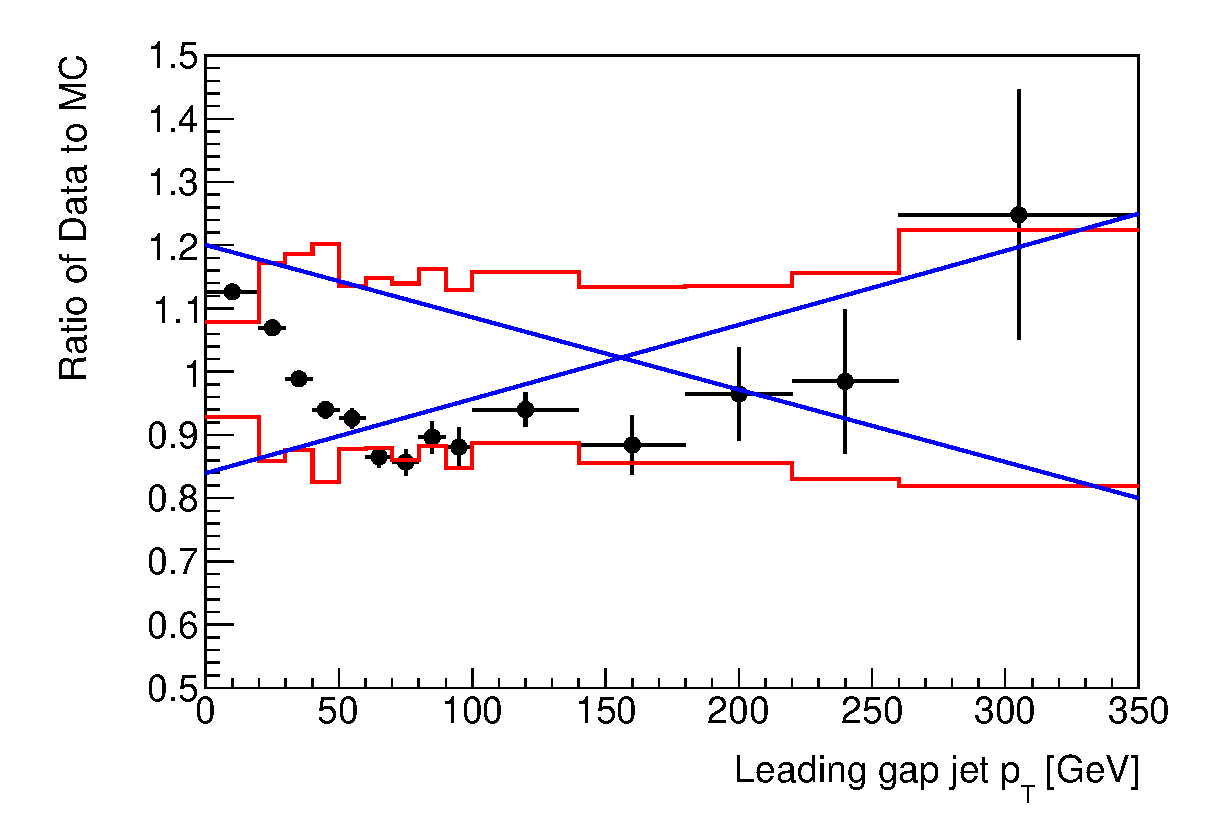
\includegraphics[width=0.8\textwidth]{figures/GBJ2/ControlPlots/Ratio___pt3.eps}
}
\caption[Comparison of the data and PYTHIA for the \pt{} of the leading gap jet]{
Ratio of the \pt{} of the leading gap jet from 2010 uncorrected data to that of the reconstructed PYTHIA sample.
The red lines show the JES uncertainty bands.
\label{GBJ2:Uncorr:pt3}}
\end{figure}


\subsection{Combined Systematics}
\label{sec:GBJ2:SysComb}

The systematics studied above were combined  with the systematic uncertainties from the unfolding process and the trigger inefficencies, to produce the overall systematic uncertainty, some of which are shown in Figures \ref{GBJ2:SysComb:GapNjet} -- \ref{GBJ2:SysComb:cos2}.
Only effects that are greater than $0.1\%$ are shown on the plots.

Figure \ref{GBJ2:SysComb:GapNjet} shows the systematic uncertainty on (a) the gap fraction and (b) the average number of jets as a function of \dy{}.
The dominant systematic is due to the JES uncertainty, while the unfolding also makes a significant contribution. 
The effect from trigger inefficencies is small, and the effects due to jet $\phi$ resolution and JER is less than $0.1\%$.


Figure \ref{GBJ2:SysComb:dphi23} shows the systematic uncertainty on the differential cross section, \dphiDist, for $2<\dy{}<3$ for (a) inclusive events and (b) gap events.
The dominant systematics are again the JES uncertainty and the unfolding. 
The effect from the $\phi$ resolution is small at low \dphi{}, but larger for high \dphi{}.

Figure \ref{GBJ2:SysComb:cos2} shows the systematic uncertainty on the \mean{\costwodphi{}} for (a) inclusive events and (b) gap events as a function of \dy{}.
For the inclusive distribution there is no overall dominant systematic. 
At low \dy{}, the uncertainty from the $\phi$ resolution is dominant, with JES and unfolding uncertainties also contributing.
At large \dy{}, the uncertainty is dominated by the JES and unfolding.
For the gap distribution, again at low \dy{} the $\phi$ resolution is the dominant systematic and at larger \dy{} all the uncertainties have an effect. 

\begin{figure}
\centering
\mbox{
              \subfigure[]{\epsfig{figure=figures/GBJ2/FinalPlots/GapFraction_dyBins.systematics.eps,width=0.5\textwidth}}\quad
              \subfigure[]{\epsfig{figure=figures/GBJ2/FinalPlots/nGapJets_dyBins.systematics.eps,width=0.5\textwidth}}\quad
                              }
\caption[Combined systematics for the gap fraction and average number of jets]{
The combined systematics for (a) the gap fraction and (b) the average number of jets in the dijet rapidity region as a function of \dy{}.
The combined systematics are from unfolding, trigger inefficencies, JES uncertainty, JER and jet $\phi$ resolution.
Only systematics with an effect greater than $0.1\%$ are displayed.
\label{GBJ2:SysComb:GapNjet}}
\end{figure}
\begin{figure}
\centering
\mbox{
              \subfigure[]{\epsfig{figure=figures/GBJ2/FinalPlots/CrossSection.Inclusive.DPhiBins.2dY3.systematics.eps,width=0.5\textwidth}}\quad
              \subfigure[]{\epsfig{figure=figures/GBJ2/FinalPlots/CrossSection.Gap.DPhiBins.2dY3.systematics-Edit.eps,width=0.5\textwidth}}\quad
                              }

\caption[Combined systematics for \dphiDist{}]{
The combined systematics for \dphiDist{}  for (a) inclusive events and (b) gap events for  $2<\dy{}<3$.
The combined systematics are from unfolding, trigger inefficencies, JES uncertainty, JER and jet $\phi$ resolution.
Only systematics with an effect greater than $0.1\%$ are displayed.
\label{GBJ2:SysComb:dphi23}}
\end{figure}


\begin{figure}
\centering
\mbox{
              \subfigure[]{\epsfig{figure=figures/GBJ2/FinalPlots/CosTwoDeltaPhiInclusive_dyBins.systematics.eps,width=0.5\textwidth}}\quad
              \subfigure[]{\epsfig{figure=figures/GBJ2/FinalPlots/CosTwoDeltaPhiGap_dyBins.systematics.eps,width=0.5\textwidth}}\quad
                              }
\caption[Combined systematics for \mean{\costwodphi{}}]{
The combined systematics for the \mean{\costwodphi{}} as a function of \dy{}  for (a) inclusive events and (b) gap events.
The combined systematics are from unfolding, trigger inefficencies, JES uncertainty, JER and jet $\phi$ resolution.
Only systematics with an effect greater than $0.1\%$ are displayed.
\label{GBJ2:SysComb:cos2}}
\end{figure}


\section{Assessment of Data vs MC Before Unfolding}
\label{sec:GBJ2:Uncorr}
This section presents the data compared to the reconstructed PYTHIA sample.
Figures \ref{GBJ2:Uncorr:Incl_Gap} -- \ref{GBJ2:Uncorr:Q0} show the uncorrected data compared to PYTHIA.
The PYTHIA error bands are the quadrature sum of the statistical error and the JES uncertainty bands. 

Figure \ref{GBJ2:Uncorr:Incl_Gap} shows (a) the gap fraction and (b) the mean number of jets in the region bounded by the dijet system, as a function of \dy{}.
The gap fraction measured from data falls as a function of \dy{}, up to $\dy{}>5.5$ where it starts to level off.
The PYTHIA gap fraction curve is consistently below the data up to a $\dy{}=6.5$.
PYTHIA then rises for the larges \dy{} bins, and has a higher gap fraction for $\dy{}>7$. 
The mean multiplicity of jets in the rapidity region increases as a function of \dy{}, to a peak of about $1.2$ at $\dy{}=7$, and then plateaus.
Both the flattening out of the gap fraction and the plateau in the mean number of jets could be due to PDF effects, such as those seen in the previous analysis for dijets with large \dy{} and \ptb{}.


Figures \ref{GBJ2:Uncorr:dphi23}, \ref{GBJ2:Uncorr:dphi45}, and \ref{GBJ2:Uncorr:dphi78} show \dphidyDist{} for $2<\dy{}<3$, $4<\dy{}<5$, and $7<\dy{}<8$,  respectively, for (a) inclusive events and (b) gap events.
PYTHIA does not describe the data particularly well, especially at high \dphi{} for  $2<\dy{}<3$ and $4<\dy{}<5$ slices where it is about $20\%$ below the data.
In the  $7<\dy{}<8$ slice, the PYTHIA results are still consistently below the data, but they agree within the JES uncertainty band.
The cross-section from PYTHIA does not agree with the measured cross-section, as there are large uncertainties in the leading order plus leading logarithm cross-section used by PYTHIA.

Figures \ref{GBJ2:Uncorr:cos} and \ref{GBJ2:Uncorr:cos2} show the \mean{\cosdphi{}} and \mean{\costwodphi{}} variables respectively, as a function of the dijet separation, \dy{}, for (a) inclusive and (b) gap events.
A \mean{\cosdphi{}} value of 1 corresponds to perfectly back-to-back jets in azimuth.
The \mean{\cosdphi{}} distribution for the inclusive events have a value of about $0.94$ for $\dy{}<2$.
As the $\dy{}$ increases, the jets become less back-to-back and the value of \mean{\cosdphi{}} falls and then levels off at a value of about $0.86$ for $\dy{}=6$.
As the $\dy{}$ increases, the available phase space to emit into is larger due to the jets being at very high energies.
For the gap events, the \mean{\cosdphi{}} at low \dy{} starts at a similar level to the inclusive events, but then slowly rises to a maximum of about $0.96$.
When the \dy{} is low, emissions can fall outside the rapidity region, but as the \dy{} increases this region becomes smaller, and the jet veto is stopping hard emission into the rapidity region, thus the dijets are more back-to-back.
The PYTHIA distribution show a slightly different shape from the data.
At both low and high \dy{}, the \mean{\cosdphi{}} for PYTHIA is higher than the data for both gap and inclusive events. 
In the range $2<\dy{}<5.5$, PYTHIA describes the data well.
The shape of the \mean{\costwodphi{}} distribution has a similar explanation to the \mean{\cosdphi{}} distribution, and shows similar features.
For both inclusive and gap events, PYTHIA's description of \mean{\costwodphi{}} is too low at low \dy{} and too high at high \dy{}.

Figure \ref{GBJ2:Uncorr:Q0} shows the gap fraction as a function of the jet veto scale, \qz{}, for the \dy{} ranges $2<\dy{}<3$, $4<\dy{}<5$, and $7<\dy{}<8$.
As \qz{} is increased, fewer events are defined as gap events, until at high \qz{} the gap fraction is at $1.0$.
In the range $2<\dy{}<3$, the PYTHIA gap fraction is lower than the data for $\qz{}<50$ GeV, though it is within the JES uncertainty.
In the range $4<\dy{}<5$, the PYTHIA gap fraction describes the data well for the full \qz{} range.
For dijets within the range $7<\dy{}<8$, the PYTHIA gap fraction is higher than the data until both gap fractions plateau at $1.0$.

\begin{figure}
\centering
\mbox{
              \subfigure[]{\epsfig{figure=figures/GBJ2/ControlPlots/Smeared__GapFraction_deltaY.eps,width=0.5\textwidth}}\quad
              \subfigure[]{\epsfig{figure=figures/GBJ2/ControlPlots/Smeared__prof_deltaY_njets.eps,width=0.5\textwidth}}\quad
                              }
\caption[Comparison of the data and PYTHIA for the gap fraction and mean number of jets]{
(a) The gap fraction  and (b) the mean number of jets in the rapidity region bounded by the dijet system as a function of \dy{} for 2010 uncorrected data (black points) and reconstructed PYTHIA sample (red points).
\label{GBJ2:Uncorr:Incl_Gap}}
\end{figure}



\begin{figure}
\centering
\mbox{
              \subfigure[]{\epsfig{figure=figures/GBJ2/ControlPlots/Smeared__dPhi__2_3.eps,width=0.5\textwidth}}\quad
              \subfigure[]{\epsfig{figure=figures/GBJ2/ControlPlots/Smeared__dPhi_gap__2_3.eps,width=0.5\textwidth}}\quad
                              }
\caption[Comparison of the data and PYTHIA for \dphidyDist{} with $2<\dy{}<3$]{
\dphidyDist{} for (a) inclusive events and (b) gap events for a dijet separation, \dy{} of 2-3 for 2010 uncorrected data (black points) and reconstructed PYTHIA sample (red points).
\label{GBJ2:Uncorr:dphi23}}
\end{figure}


\begin{figure}
\centering
\mbox{
              \subfigure[]{\epsfig{figure=figures/GBJ2/ControlPlots/Smeared__dPhi__4_5.eps,width=0.5\textwidth}}\quad
              \subfigure[]{\epsfig{figure=figures/GBJ2/ControlPlots/Smeared__dPhi_gap__4_5.eps,width=0.5\textwidth}}\quad
                              }
\caption[Comparison of the data and PYTHIA for \dphidyDist{} with $4<\dy{}<5$]{
\dphidyDist{} for (a) inclusive events and (b) gap events for a dijet separation, \dy{} of 4-5 for 2010 uncorrected data (black points) and reconstructed PYTHIA sample (red points).
\label{GBJ2:Uncorr:dphi45}}
\end{figure}



\begin{figure}
\centering
\mbox{
              \subfigure[]{\epsfig{figure=figures/GBJ2/ControlPlots/Smeared__dPhi__7_8.eps,width=0.5\textwidth}}\quad
              \subfigure[]{\epsfig{figure=figures/GBJ2/ControlPlots/Smeared__dPhi_gap__7_8.eps,width=0.5\textwidth}}\quad
                              }
\caption[Comparison of the data and PYTHIA for \dphidyDist{} with $7<\dy{}<8$]{
\dphidyDist{} for (a) inclusive events and (b) gap events for a dijet separation, \dy{} of 7-8 for 2010 uncorrected data (black points) and reconstructed PYTHIA sample (red points).
\label{GBJ2:Uncorr:dphi78}}
\end{figure}



\begin{figure}
\centering
\mbox{
              \subfigure[]{\epsfig{figure=figures/GBJ2/ControlPlots/Smeared__cosdPhi_deltaY.eps,width=0.5\textwidth}}\quad
              \subfigure[]{\epsfig{figure=figures/GBJ2/ControlPlots/Smeared__cosdPhi_deltaY_gap.eps,width=0.5\textwidth}}\quad
                              }
\caption[Comparison of the data and PYTHIA for \cosdphi{}]{
\mean{\cosdphi{}} as a function of \dy{} for (a) inclusive and (b) gap events for 2010 uncorrected data (black points) and reconstructed PYTHIA sample (red points).
\label{GBJ2:Uncorr:cos}}
\end{figure}


\begin{figure}
\centering
\mbox{
              \subfigure[]{\epsfig{figure=figures/GBJ2/ControlPlots/Smeared__cos2dPhi_deltaY.eps,width=0.5\textwidth}}\quad
              \subfigure[]{\epsfig{figure=figures/GBJ2/ControlPlots/Smeared__cos2dPhi_deltaY_gap.eps,width=0.5\textwidth}}\quad
                              }
\caption[Comparison of the data and PYTHIA for \costwodphi{}]{
\mean{\costwodphi{}} as a function of \dy{} for (a) inclusive and (b) gap events for 2010 uncorrected data (black points) and reconstructed PYTHIA sample (red points).
\label{GBJ2:Uncorr:cos2}}
\end{figure}

\begin{figure}
\centering
\mbox{
      \subfigure[]{\epsfig{figure=figures/GBJ2/ControlPlots/Smeared2_3__Q0,width=0.5\textwidth}}\quad
      \subfigure[]{\epsfig{figure=figures/GBJ2/ControlPlots/Smeared4_5__Q0,width=0.5\textwidth}}\quad
}
\mbox{
      \subfigure[]{\epsfig{figure=figures/GBJ2/ControlPlots/Smeared7_8__Q0,width=0.5\textwidth}}\quad
}
\caption[Comparison of the data and PYTHIA for the gap fraction as a function of \qz{}]{
The gap fraction against \qz{} for (a) $2<\dy{}<3$, (b) $4<\dy{}<5$ and (c) $7<\dy{}<8$ for 2010 uncorrected data (black points) and reconstructed PYTHIA sample (red points).
\label{GBJ2:Uncorr:Q0}}
\end{figure}


%\section{Corrected Data}
\label{sec:GBJ2:FinalPlots}

First, the corrected data, with the systematic uncertainties discussed, is first compared to some common MC generators in Figures \ref{GBJ2:FinalPlots:GapFracLO} and \ref{GBJ2:FinalPlots:NJetLO}.
The MC generators chosen for the comparison are PYTHIA, HERWIG++ and SHERPA. 

Figure \ref{GBJ2:FinalPlots:GapFracLO} shows (a) the gap fraction against \dy{} for the corrected data and the MC generators, and (b) shows the ratio of the MCs to the data.
The gap fraction from data reduces as a function of \dy{}, but for $\dy{}>5.5$ it starts to level off. 
In general, PYTHIA gives slightly too low a gap fraction at low \dy{} but improves at larger \dy{}. 
HERWIG overlaps the data  at low \dy{} but from \dy{} of 3 onwards it diverges from the data giving too low a gap fraction. 
HERWIG has large statistical error bars, and to get a full understanding of the shape higher statistics sample need to be generated.
SHERPA agrees quite well with the data, but with some deviations at large \dy{}.

Figure \ref{GBJ2:FinalPlots:NJetLO} shows (a) the average number of jets in the dijet rapidity region against \dy{} for the corrected data and the MC generators, and (b) shows the ratio of the MCs to the data.
As with the gap fraction, PYTHIA agrees with the data  matching the rise and position of the peak, but underestimates the data at large \dy{}.
HERWIG agrees with the data at low \dy{}, but diverges at larger \dy{}.
Due to the low statistics, it is hard to conclude if the HERWIG flattens, or weather it continues to rise.
SHERPA on the whole agrees well with the data, but around a \dy{} of 4--7 underestimates the number of jets in the rapidity region.

The corrected data is compared the theory predictions from HEJ and POWHEG. 
The theory predictions are presented as a band to represent the theoretical uncertainty, which was found by varying both the renormalisation and factorisation scale and also the choice of PDF.
Two POWHEG curves are shown which have the different parton showering, hadronization and underlying event of PYTHIA and HERWIG. 
The HEJ events have been passed through Ariadne, which is a \pt{} ordered parton shower. 


Figure \ref{GBJ2:FinalPlots:GapFrac} shows (a) the gap fraction against \dy{} for the corrected data and the theoretical predictions, and (b) shows the ratio of the predictions to the data.
There is significant differences between the three theoretical predictions and the data.
POWHEG + PYTHIA gives the best agreement with data, and while the gap fraction is slightly lower than the data, it agrees in most bins. 
The plateau in the data is also observed in the POWHEG + PYTHIA curve.
Conversely, POWHEG + HERWIG has too low a gap fraction from from about a \dy{} of 2.
The HEJ prediction also gives too low a gap fraction, but not as far from the data as the POWHEG + HERWIG curve.
Given that most of the events will have a low \ptb{} without a large imbalance (cuts on $pt{}_1$ and $pt{}_2$ are similar) it is surprising that HEJ does not perform well, especially when compared to the previous measurement.
This maybe due to the change in kinematics cuts in this analysis, or due to the effect of passing the events through Ariadne.
Also to be noted, in the previous analysis the gap fraction for data only flattened out in large \ptb{} slices. 
In this analysis there is not a particularly high \ptb{} cut, and a flattening out is observed.
A flattening out could be due to PDF effects, for instance if both jets have an energy of  $3.5$ TeV, then no emission can occur.
A flattening out is also intrinsic with a colour singlet exchange (get paper off Andy).
This needs to be analysed with a MC that has a model for  colour singlet exchange.


Figure \ref{GBJ2:FinalPlots:nJets} shows (a) the average number of jets in the dijet rapidity region against \dy{} for the corrected data and the theoretical predictions, and (b) shows the ratio of the predictions to the data.
The mean multiplicity of jets in the rapidity region increases as a function of \dy{}, to a peak of $\sim1.2$ at $\dy{}=7$, and then plateau's.
POWHEG + PYTHIA agrees well best with the data, overlapping in most \dy{} bins and has a very good agreement at the plateau.
HEJ agrees with the data well until a \dy{} of 4, but then gives too many jets, and does not replicate the plateau observed in the data. 
In the previous analysis, HEJ gave two low activity, which would indicate that Ariadne is increasing the amount of activity, but perhaps too much.
POWHEG + HERWIG only agrees with data at the very lowest \dy{} bins, then has too many jets in the rapidity region for larger \dy{} and but it does have a plateau at large \dy{}.

Figure \ref{GBJ2:FinalPlots:Q0} shows (a) the gap fraction as a function of \qz{} for the three standard \dy{} slices for the corrected data and the theoretical predictions, and (b) shows the ratio of the predictions to the data.
All the theoretical predictions agree with data at large \qz{} where the gap fraction is one, this is because the \qz{} will, most of the time, be set above the \pt{} of the leading jets, so there cannot be any other jets in the event with \pt{} greater than \qz{}
HEJ gives too low a gap fraction in the lower \qz{} region, especially for the higher \dy{} ranges, which was also seen in the gap fraction against \dy{} in Figure \ref{GBJ2:FinalPlots:GapFrac}.
POWHEG + HERWIG has too low a gap fraction at the low \qz{} region for all \dy{} slices, but as with HEJ, it get worse at larger \dy{} ranges.
POWHEG + PYTHIA gives the best description of the data, but still getting too low a gap fraction for $30<\qz{}<60$ for the lowest \dy{} range.


%Figure \ref{GBJ2:FinalPlots:dphi_Incl} shows (a) the differential cross section as a function of \dphi{} for the three standard \dy{} slices for the corrected data and the theoretical predictions, and (b) shows the ratio of the predictions to the data.
%For the low \dy{} slice, all the theoretical predictions poorly match the data at low \dphi{}, but improve for larger \dphi{}.
%HEJ does particularly well in the 4--5 \dy{} slice, agreeing with the data for all \dphi{}.
%Both POWHEG + HERWIG and POWHEG + PYTHIA have a larger cross section for all but the largest two \dphi{} bins for the 4--5 \dy{} slice.
%In the 7--8 \dy{} slice, both POWHEG + HERWIG and POWHEG + PYTHIA agree with the data within the systematic uncertainty band, which is quite large in this slice.
%HEJ how too low a cross section in the 7--8 \dy{} slice. 

Figure \ref{GBJ2:FinalPlots:Cos} shows the \mean{\cosdphi{}} as a function of \dy{} for (a) inclusive events and (c) gap events with the ratios of the theoretical predictions to the data in (b) and (d) respectively. 
A \mean{\cosdphi{}} value of one corresponds to perfectly back-to-back in azimuth jets.
The \mean{\cosdphi{}} distribution for the inclusive events shows a value of $ \mean{\cosdphi{}}\sim0.95$ for $\dy{}<3$.
As the $\dy{}$ increase the jets become less back-to-back and the \mean{\cosdphi{}} falls.
As the $\dy{}$ increase the available phase-space to emit into is larger due to the jet being at very high energies.
For the gap events, the mean{\cosdphi{}} at low \dy{} starts at a similar level to the inclusive events, but then slowly rises.
When the \dy{} is low, emissions can fall outside the rapidity region, but as the \dy{} increases this region becomes smaller, and the jet veto is stopping hard emission into the rapidity region.
For the inclusive events, all three predictions undershoot the data for $3.5<\dy{}<6$.
While HEJ agrees in quite a few bins, the shape is steeper than observed in data.
Both POWHEG + HERWIG and POWHEG + PYTHIA have a similar shape to the data, but the overall scale is a bit low.
For the gap events, all three predictions have a similar shape to the data, but HEJ's overall scale is on the high side of the data, and the POWHEG + PYTHIA and  POWHEG + HERWIG are slightly below the data.
This observable does not discriminate well between the different theoretical predictions. 

Figure \ref{GBJ2:FinalPlots:Cos2} shows the \mean{\costwodphi{}} as a function of \dy{} for (a) inclusive events and (c) gap events with the ratios of the theoretical predictions to the data in (b) and (d) respectively. 
Similar results to the \mean{\cosdphi{}} are seen for \mean{\costwodphi{}}.
For the inclusive events, the HEJ curve has a steeper shape, crossing the data at $\dy{}\sim2.5$. 
The POWHEG + HERWIG and POWHEG + PYTHIA fall below the data throughout \dy{}.
For the gap events, HEJ is above the data, except at large \dy{} where there are large uncertainties.
Both the POWHEG + HERWIG and POWHEG + PYTHIA fall below the data.

For the azimuthal decorralation observables, POWHEG + PYTHIA again agrees best with the data, matching the shape of the data, even if the overall scale is a bit low.


\begin{figure}
\centering
\mbox{
              \subfigure[]{\epsfig{figure=figures/GBJ2/FinalPlots/LO_GapFraction_dyBins.eps,width=0.5\textwidth}}\quad
              \subfigure[]{\epsfig{figure=figures/GBJ2/FinalPlots/LO_GapFraction_dyBins_Ratio-Edit.eps,width=0.5\textwidth}}\quad
                              }
\caption[]{
(a) The gap fraction as a function of \dy{}.  
The 2010 corrected data (black points) is shown with statistical (black error bars) and systematic (yellow error band) error bands against leading order MCs of PYTHIA, HERWIG++ and SHERPA.
The ratio to the data for (a)  is shown in (b).
\label{GBJ2:FinalPlots:GapFracLO}}
\end{figure}

\begin{figure}
\centering
\mbox{
              \subfigure[]{\epsfig{figure=figures/GBJ2/FinalPlots/LO_nGapJets_dyBins.eps,width=0.5\textwidth}}\quad
              \subfigure[]{\epsfig{figure=figures/GBJ2/FinalPlots/LO_nGapJets_dyBins_Ratio-Edit.eps,width=0.5\textwidth}}\quad
                              }
\caption[]{
(a) The average number of jets in the dijet rapidity region as a function of \dy{}.  
The 2010 corrected data (black points) is shown with statistical (black error bars) and systematic (yellow error band) error bands against leading order MCs of PYTHIA, HERWIG++ and SHERPA.
The ratio to the data for (a) is shown in (b).
\label{GBJ2:FinalPlots:NJetLO}}
\end{figure}

\begin{figure}
\centering
\mbox{
              \subfigure[]{\epsfig{figure=figures/GBJ2/FinalPlots/GapFraction_dyBins.eps,width=0.5\textwidth}}\quad
              \subfigure[]{\epsfig{figure=figures/GBJ2/FinalPlots/GapFraction_dyBins_Ratio.eps,width=0.5\textwidth}}\quad
                              }
\caption[]{
(a) The gap fraction as a function of \dy{}.  
The 2010 corrected data (black points) is shown with statistical (black error bars) and systematic (yellow error band) error bands against HEJ and POWHEG predictions.
The ratio of the theoretical predictions to the data is shown in (b).
\label{GBJ2:FinalPlots:GapFrac}}
\end{figure}



\begin{figure}
\centering
\mbox{
              \subfigure[]{\epsfig{figure=figures/GBJ2/FinalPlots/nGapJets_dyBins.eps,width=0.5\textwidth}}\quad
              \subfigure[]{\epsfig{figure=figures/GBJ2/FinalPlots/nGapJets_dyBins_Ratio.eps,width=0.5\textwidth}}\quad
                              }
\caption[]{
(a) The average number of jets in the dijet rapidity region as a function of \dy{}.  
The 2010 corrected data (black points) is shown with statistical (black error bars) and systematic (yellow error band) error bands against HEJ and POWHEG predictions.
The ratio to the data for (a) is shown in (b). 
\label{GBJ2:FinalPlots:nJets}}
\end{figure}

\begin{figure}
\centering
\mbox{
              \subfigure[]{\epsfig{figure=figures/GBJ2/FinalPlots/GapFraction_Q0-Edit.eps,width=0.5\textwidth}}\quad
              \subfigure[]{\epsfig{figure=figures/GBJ2/FinalPlots/GapFraction_Q0_Ratio.eps,width=0.5\textwidth}}\quad
                              }
\caption[]{
The gap fraction as a function of \qz{} for the three standard \dy{} ranges.  
The 2010 corrected data (black points) is shown with statistical (black error bars) and systematic (yellow error band) error bands against HEJ and POWHEG predictions.
The ratio of the theoretical predictions to the data is shown in (b).
\label{GBJ2:FinalPlots:Q0}}
\end{figure}

\begin{figure}
\centering
\mbox{
              \subfigure[]{\epsfig{figure=figures/GBJ2/FinalPlots/CrossSection.Inclusive.DPhiBins.AlldY.eps,width=0.5\textwidth}}\quad
              \subfigure[]{\epsfig{figure=figures/GBJ2/FinalPlots/CrossSection.Inclusive.DPhiBins.AlldY.Ratio.eps,width=0.5\textwidth}}\quad
                              }
\caption[]{
The differential cross section as a function of \dphi{} for inclusive events for the three standard \dy{} ranges.  
The 2010 corrected data (black points) is shown with statistical (black error bars) and systematic (yellow error band) error bands against HEJ and POWHEG predictions.
The ratio of the theoretical predictions to the data is shown in (b).
\label{GBJ2:FinalPlots:dPhi_Incl}}
\end{figure}

\begin{figure}
\centering
\mbox{
              \subfigure[]{\epsfig{figure=figures/GBJ2/FinalPlots/CrossSection.Gap.DPhiBins.AlldY.eps,width=0.5\textwidth}}\quad
              \subfigure[]{\epsfig{figure=figures/GBJ2/FinalPlots/CrossSection.Gap.DPhiBins.AlldY.Ratio.eps,width=0.5\textwidth}}\quad
                              }
\caption[]{
The differential cross section as a function of \dphi{} for inclusive events for the three standard \dy{} ranges.  
The 2010 corrected data (black points) is shown with statistical (black error bars) and systematic (yellow error band) error bands against HEJ and POWHEG predictions.
The ratio of the theoretical predictions to the data is shown in (b).
\label{GBJ2:FinalPlots:dPhi_Gap}}
\end{figure}


\begin{figure}
\centering
\mbox{
              \subfigure[]{\epsfig{figure=figures/GBJ2/FinalPlots/CosDeltaPhiInclusive_dyBins.eps,width=0.5\textwidth}}\quad
              \subfigure[]{\epsfig{figure=figures/GBJ2/FinalPlots/CosDeltaPhiInclusive_dyBins_Ratio.eps,width=0.5\textwidth}}\quad
                              }
\mbox{
              \subfigure[]{\epsfig{figure=figures/GBJ2/FinalPlots/CosDeltaPhiGap_dyBins.eps,width=0.5\textwidth}}\quad
              \subfigure[]{\epsfig{figure=figures/GBJ2/FinalPlots/CosDeltaPhiGap_dyBins_Ratio.eps,width=0.5\textwidth}}\quad
                              }
\caption[]{
The average \cosdphi{} as a function of \dy{} for (a) inclusive events and (c) gap events for the three standard \dy{} ranges.  
The 2010 corrected data (black points) is shown with statistical (black error bars) and systematic (yellow error band) error bands against HEJ and POWHEG predictions.
The ratio to the data for (a) and (c) is shown in (b) and (d) respectively.
\label{GBJ2:FinalPlots:Cos}}
\end{figure}

\begin{figure}
\centering
\mbox{
              \subfigure[]{\epsfig{figure=figures/GBJ2/FinalPlots/CosTwoDeltaPhiInclusive_dyBins.eps,width=0.5\textwidth}}\quad
              \subfigure[]{\epsfig{figure=figures/GBJ2/FinalPlots/CosTwoDeltaPhiInclusive_dyBins_Ratio.eps,width=0.5\textwidth}}\quad
                              }
\mbox{
              \subfigure[]{\epsfig{figure=figures/GBJ2/FinalPlots/CosTwoDeltaPhiGap_dyBins.eps,width=0.5\textwidth}}\quad
              \subfigure[]{\epsfig{figure=figures/GBJ2/FinalPlots/CosTwoDeltaPhiGap_dyBins_Ratio.eps,width=0.5\textwidth}}\quad
                              }
\caption[]{
The average \costwodphi{} as a function of \dy{} for (a) inclusive events and (c) gap events for the three standard \dy{} ranges.  
The 2010 corrected data (black points) is shown with statistical (black error bars) and systematic (yellow error band) error bands against HEJ and POWHEG predictions.
The ratio to the data for (a) and (c) is shown in (b) and (d) respectively.
\label{GBJ2:FinalPlots:Cos2}}
\end{figure}





\chapter{Summary and Conclusions}
In this thesis a summary of two precision jet measurements are presented that aim to probe higher-order QCD phenomena by studying the amount of radiation from a dijet system.

To make precision jet measurements, a good understanding of the detector and its response to jets is vital. 
The monitoring of the calorimeter high-level trigger, which is used in the analyses to trigger events, has been detailed. 
The trigger was shown to be stable over different data periods, and problems, such as noisy cells, could be monitored and masked.
The performance of jets within the calorimeter was also assessed.
The dijet \pt{} balance method was used to extend a determination of the central jet energy scale uncertainty out to larger \dy{}, and the effect from pile-up and a closure of the method were studied. 
Additionally, some properties of jets in the transition region between the end-cap and FCal and in the FCal were studied and compared to different showering models.
The closure of the dijet \pt{} balance method and the properties of the jets in the transition region between the end-cap and FCal and in the FCal itself have been  published as an ATLAS conference note \cite{ref:EtaInter2010}.

Dijet production with a jet veto for fixed regions of phase space was studied for rapidity separations of up to six units in rapidity with average \pt{} of the dijets from 50 to 500 GeV.  
The measurement of the fraction of events that survived a jet veto were compared to PYTHIA, HERWIG++ and ALPGEN event generators as well as to next-to-leading-order predictions from POWHEG, interfaced with the partons showering from PYTHIA and HERWIG, and to a prediction using the HEJ generator.
Two different dijet selections were studied, the leading \pt{} dijet selection and the forward/backward dijet selection. 
No prediction agreed in all the areas of phase space considered.
POWHEG + PYTHIA had the best agreement with data, but differences were observed at high \dy{}.
HEJ described the data as a function of \dy{}, but only for low $\ptb{}$; at high $\ptb{}$ the gap fraction was too high.
POWHEG + HERWIG gave a poor description of the data with too low a gap fraction throughout.
The mean multiplicity of jets in the rapidity region has also been presented for the leading \pt{} dijet selection.
The activity of HEJ was significantly lower than the data for all but the lowest \dy{} bin. 
Given the agreement for the gap fraction, it seems HEJ describes the veto jet well, but does not cope well with any additional jets beyond that. 
POWHEG + HERWIG had too much activity throughout, which correlates well with the predicted gap fraction that is too low.
POWHEG + PYTHIA gave the best description of the data, although they did deviate at high \dy{}.
The results of this analysis have been published in JHEP \cite{ref:ATLASGap} as well in the ATLAS conference notes \cite{ref:GBJConf1,ref:GBJConf2}.

A preliminary analysis studying  emissions from very high rapidity separated jets was also presented, with a measurement up to a separation of eight units in rapidity.
The systematic uncertainties from the data selection and jet uncertainties were assessed.
In the analysis both the gap fraction and the mean number of jets in the rapidity region between the dijet system were studied. 
The azimuthal decorrelation variables, \dphiDist{}, \mean{\cosdphi} and \mean{\costwodphi} were also studied.
The data were compared to fully reconstructed PYTHIA.
In the high \dy{} region, the gap fraction levelled off in the data. 
This feature was only observed at high \pt{} in the previous analysis. 
The shape of the PYTHIA distributions in the variables \mean{\cosdphi} and \mean{\costwodphi} were different to the data, with the data having a lower value at very high \dy{}.  
The results of this second analysis are currently being reviewed internally by the ATLAS collaboration \cite{ref:GBJInternal}.





\bibliographystyle{mnras}
\bibliography{references}
\end{document}
